
\documentclass[a4paper,11.5pt]{article}
\usepackage[textwidth=170mm, textheight=230mm, inner=20mm, top=20mm, bottom=30mm]{geometry}
\usepackage[normalem]{ulem}
\usepackage[utf8]{inputenc}
\usepackage[T1]{fontenc}
\PassOptionsToPackage{defaults=hu-min}{magyar.ldf}
\usepackage{pgfplots}
\pgfplotsset{compat=1.10}
\usepgfplotslibrary{fillbetween}
\usepackage[magyar]{babel}
\usepackage{amsmath, amsthm,amssymb,paralist,array, ellipsis, graphicx, float, bigints,tikz}
%\usepackage{marvosym}

\makeatletter
\renewcommand*{\mathellipsis}{%
	\mathinner{%
		\kern\ellipsisbeforegap%
		{\ldotp}\kern\ellipsisgap
		{\ldotp}\kern\ellipsisgap%
		{\ldotp}\kern\ellipsisaftergap%
	}%
}
\renewcommand*{\dotsb@}{%
	\mathinner{%
		\kern\ellipsisbeforegap%
		{\cdotp}\kern\ellipsisgap%
		{\cdotp}\kern\ellipsisgap%
		{\cdotp}\kern\ellipsisaftergap%
	}%
}
\renewcommand*{\@cdots}{%
	\mathinner{%
		\kern\ellipsisbeforegap%
		{\cdotp}\kern\ellipsisgap%
		{\cdotp}\kern\ellipsisgap%
		{\cdotp}\kern\ellipsisaftergap%
	}%
}
\renewcommand*{\ellipsis@default}{%
	\ellipsis@before
	\kern\ellipsisbeforegap
	.\kern\ellipsisgap
	.\kern\ellipsisgap
	.\kern\ellipsisgap
	\ellipsis@after\relax}
\renewcommand*{\ellipsis@centered}{%
	\ellipsis@before
	\kern\ellipsisbeforegap
	.\kern\ellipsisgap
	.\kern\ellipsisgap
	.\kern\ellipsisaftergap
	\ellipsis@after\relax}
\AtBeginDocument{%
	\DeclareRobustCommand*{\dots}{%
		\ifmmode\@xp\mdots@\else\@xp\textellipsis\fi}}
\def\ellipsisgap{.1em}
\def\ellipsisbeforegap{.05em}
\def\ellipsisaftergap{.05em}
\makeatother

\usepackage{hyperref}
\hypersetup{
	colorlinks = true	
}

\DeclareMathOperator{\Int}{int}
\DeclareMathOperator{\tg}{tg}
\DeclareMathOperator{\ctg}{ctg}
\DeclareMathOperator{\Th}{th}
\DeclareMathOperator{\sh}{sh}
\DeclareMathOperator{\ch}{ch}
\DeclareMathOperator{\sign}{sign}
\DeclareMathOperator{\arsh}{arsh}
\DeclareMathOperator{\arch}{arch}
\DeclareMathOperator{\arth}{arth}
\DeclareMathOperator{\arcth}{arcth}
\DeclareMathOperator{\arc}{arc}
\DeclareMathOperator{\arctg}{arc tg}
\DeclareMathOperator{\arcctg}{arc ctg}

\begin{document}
	%%%%%%%%%%%RÖVIDÍTÉSEK%%%%%%%%%%
	\setlength\parindent{0pt}
	\def\a{\textbf{a}}
	\def\b{\textbf{b}}
	\def\N{\hskip 10 true mm}
	\def\a{\textbf{a}}
	\def\b{\textbf{b}}
	\def\c{\textbf{c}}
	\def\d{\textbf{d}}
	\def\e{\textbf{e}}
	\def\gg{$\gamma$}
	\def\vi{\textbf{i}}
	\def\jj{\textbf{j}}
	\def\kk{\textbf{k}}
	\def\fh{\overrightarrow}
	\def\l{\lambda}
	\def\m{\mu}
	\def\v{\textbf{v}}
	\def\0{\textbf{0}}
	\def\s{\hspace{0.2mm}\vphantom{\beta}}
	\def\Z{\mathbb{Z}}
	\def\Q{\mathbb{Q}}
	\def\R{\mathbb{R}}
	\def\C{\mathbb{C}}
	\def\N{\mathbb{N}}
	\def\Rn{\mathbb{R}^{n}}
	\def\Ra{\overline{\mathbb{R}}}
	\def\sume{\displaystyle\sum_{n=1}^{+\infty}}
	\def\sumn{\displaystyle\sum_{n=0}^{+\infty}}
	\def\biz{\emph{Bizonyítás:\ }}
	\def\narrow{\underset{n\rightarrow+\infty}{\longrightarrow}}
	\def\limn{\displaystyle\lim_{n\to +\infty}}
	%	\def\definition{\textbf{Definíció:\ }}
	%	\def\theorem{\textbf{Tétel:\ }}
	%\def\note{\emph{Megjegyzés:\ }}
	%\def\example{\textbf{Példa:\ }} 
	
	\theoremstyle{definition}
	\newtheorem{theorem}{Tétel}[subsubsection] % reset theorem numbering for each chapter
	
	\theoremstyle{definition}
	\newtheorem{definition}[theorem]{Definíció} % definition numbers are dependent on theorem numbers
	\newtheorem{example}[theorem]{Példa} % same for example numbers
	\newtheorem{exercise}[theorem]{Házi feladat} % same for example numbers
	\newtheorem{note}[theorem]{Megjegyzés} % same for example numbers
	\newtheorem{task}[theorem]{Feladat} % same for example numbers
	\newtheorem{revision}[theorem]{Emlékeztető} % same for example numbers
	%%%%%%%%%%%%%%%%%%%%%%%%%%%%%%%%%
	\begin{center}
		{\LARGE\textbf{Analízis 3. A szakirány}}
		\smallskip

		{\Large Gyakorlati jegyzet}

		\smallskip
		1-6. óra.
	\end{center}
	A jegyzetet \textsc{Umann} Kristóf készítette \textsc{Filipp} Zoltán István gyakorlatán. (Utoljára frissítve: \today)	\tableofcontents
	\section{Információk a gyakorlattal kapcsolatban}
	\begin{compactitem}
		\item emial: filipp@numanal.inf.elte.hu
		\item szoba: 2-316A
		\item Telefonszám: 06-70-332-01-41
		\item Cím: \url{numanal/~filipp}, analízis 3, azon belül A.
		\item várható majd kötelezően beadandó integrálszámítás
		\item 8:30 kezdés
		\item 7. héten első zh, 13. hét második zh
		\item egy csütörtök el fog maradni, de pótolva lesz
		\item Konzi: szerda 9-10
	\end{compactitem}
	Ami a honlapon található:
	\begin{compactitem}
		\item Gyakorlati anyag
		\item Gyemidovics tankönyv (III. fejezet) (és ennek eredményei külön fájlban)
		\item Bolyai sorozat (integrálszámítás és többváltozós analízis)
		\item Ajánlottak mint Szili analízis feladat gyűjteménye és integráltáblázata.
		\item Károlyi Katalin
	\end{compactitem}
	\section{Integrálszámítás}
	\subsection{Bevezető}
	\begin{revision}
		(Primitív függvény)\quad Legyen $\emptyset\not=I\subset\R$ nyílt intervallum, és $f:I\to\R$ fv. Ha 
		\[\exists F:I\to\R, \quad F\in D\quad  \text{és}\quad  F'(x)=f(x) \quad (\forall x\in I),\]
		akkor azt mondjuk hogy $F$ az $f$ egy primitív függvénye.
	\end{revision}
	Nem minden függvény rendelkezik primitív függvénnyel, pl.: $\sign(x)$, mert az 1/2-et nem veszi fel sehol.
	\begin{note}
	$f(x)=x^2,\quad x\in I:=\R;\quad \Rightarrow\quad F(x)=\frac{1}{3}x^3\quad (x\in\R)$, mert $\left(\frac{1}{3}x^3\right)'=\frac{1}{3}3x^2=x^2$.
	
	Ezek is primitív függvényei $f$-nek $(x\in\R)$:
	\[ F_1(x):=\frac{1}{3}x^3+1,\quad  F_{34}(x):=\frac{1}{3}x^3+34 \]
	Általánoságban
	\[ F(x):=\frac{1}{3}x^3+c\quad (c, x\in\R) \]
	\end{note}
	Két primitív függvény konstansban térhet csak el. Ez alapján megállapítható, hogy ha létezik primitív függvény, végtelen sok lehet belőlük.
	\begin{note}
		Ha van $f$-nek primitív függvénye, akkor
		\[  \int f(x)\,dx:=\{F:I\to\R~|~F\in D \text{\quad és\quad } F'=f \} =F(x) + c \]
		az $f$ primitív függvényeinek a halmaza, vagy az $f$ határozatlan integrálja
	\end{note}
	Mindig meg kell adnunk az $I$ intervallumot.
	
	Néha az is kérdés lehet, egy függvény melyik pontban tűnik el, azaz nem mindig a 0ra vagyunk kíváncsiak.
	\begin{task}
		Adjuk meg azt az $F$-et, melyre $F(1)=2$
	\end{task}
	%TODO ábra 1
	\begin{revision}
		$f:$idő$\to$távolság
		
		Ilyenkor mit jelent $f'$? az a sebesség, míg $f''$ a gyorsulás. Ott gyakran vannak olyan feltételek, hogy a kezdősebesség legyen 2 ($f(1)=2$)
		
		Ehhez a fenti feladatot példaképp véve $\frac{1}{3}^3+c=2$ egyenletet kell megoldani $\quad \Rightarrow\quad c=\frac{5}{3}$.
	\end{revision}
	Tehát:
	\[ F(x)=\frac{x^3}{3}+\frac{5}{3} \]
	\begin{task}$(x\in\R$)
		\[\int \cos x\,dx=\sin x+c\quad (c\in\R) \]
	\end{task}
	\begin{task}
		\[ (\arccos\tan x)' =\frac{1}{1+x^2}\quad \Rightarrow\quad \int\frac{1}{1+x^2}\,dx=\arctan x + c\quad (x,c\in \R) \]
	\end{task}
	\begin{task} $x\in(-1,1)$
		\[ \int\frac{1}{\sqrt{1-x^2}}\,dx=\arc\sin x + c \quad (c\in \R) \]
	\end{task}
	\subsection{Alapintegrálok és ezekre vezethető típusok}
	Szokás úgy is hívni hogy antiderivált, mert az annak az ellentettje.
	\begin{task}$(x\in\R)$
		\[\int(6x^3-2x+1)\,dx\]
	\end{task}
	Emlékezzünk vissza a műveleti tételekre. Az integrál lineáris, így az integráltat integráltak összegére bonthatjuk és a konstansokat is ki tudjuk \textit{,,cuppantani''}:
	\[ 6\cdot\int x^3\,dx-2\cdot\int x\,dx+\int1\,dx=6\cdot\frac{x^4}{4}-2\cdot\frac{x^2}{2}+x+c\quad (c\in\R) \]
	\begin{theorem}
		Általános integrálfüggvény:
		\[ \int x^\alpha\,dx=\frac{x^{\alpha+1}}{\alpha+1}+c\quad (x>0,\quad  c,\alpha\in\R) \]
		Ha $\alpha\not=-1$.
	\end{theorem}
	\begin{task}Határozzuk meg az $f(x):=\frac{1}{x}$ integráltját. Ezt esetekre kell bontani (szétválasztani az értelmezési tartományt intervallumokra), legyen az első $x>0$. Bár $\R\setminus\{0\}$ is jó választás értelmezési tartománynak, de az nem intervallum.
		\[ \int\frac{1}{x}\,dx=\ln x+c\quad (c\in\R) \]
		Második eset $x\in(-\infty,0)=:I$:
		\[ \int\frac{1}{x}\,dx=\ln(-x)+c\quad (c\in\R),\quad \text{ui.}\quad (\ln(-x))'=\frac{1}{-x}(-x)'=-\frac{1}{x}\cdot(-1)=\frac{1}{x} \]
	\end{task}
	\begin{note}
		az előző két feladat összefoglalható úgy, hogy 
		\[ \int\frac{1}{x}\,dx=\ln|x|+c\quad (c\in\R, x\in(-\infty,0)\quad \text{vagy}\quad (0,+\infty) \]
	\end{note}
	\begin{task}$x>0$
		\[ \int\sqrt{x\sqrt{x\sqrt{x}}}\,dx=\int x^\frac{1}{2}\cdot x^\frac{1}{4}\cdot x^\frac{1}{8}\, dx=\int x^{\frac{1}{2}+\frac{1}{4}+\frac{1}{8}}\,dx=\int x^{\frac{7}{8}}\,dx=\frac{x^{\frac{7}{8}+1}}{\frac{7}{8}+1}+c=\frac{8}{15}\cdot\sqrt[8]{x^{15}}+c\quad (c\in\R) \]
	\end{task}
	\begin{note}
		Ha szorzat van csinálj összeget, ha összeg van cisnálj szorzatot
	\end{note}
	\begin{task}
		\[ \int\frac{(x+1)^2}{\sqrt{x}}\,dx=\int\frac{x^2+2x+1}{x^\frac{1}{2}}\,dx=\int\frac{x^2}{x^{\frac{1}{2}}}\,dx+2\int\frac{x}{x^\frac{1}{2}}\,dx+\int\frac{1}{x^\frac{1}{2}}\,dx=\int x^\frac{3}{2}\,dx+2\int x^\frac{1}{2}\,dx+\int x^{-\frac{1}{2}}\,dx= \]
		\[=\frac{x^{\frac{3}{2}+1}}{\frac{3}{2}+1}+2\frac{x^{\frac{1}{2}+1}}{\frac{1}{2}+1}x+\frac{x^{-\frac{1}{2}+1}}{-\frac{1}{2}+1}+c\quad (c\in\R) =\frac{2}{5}\cdot\sqrt{x^5}+\frac{4}{3}\sqrt{x^3}+2\sqrt{x}+c \]
	\end{task}
	\begin{center}
		\textit{,,Integrálni úgy kell hogy nézed, nézed, nézed, és aztán rájössz.''}
		
		/Filipp/
	\end{center}
	\begin{note}
		A fenti módszer hívjuk az összegre bontás módszerének.
	\end{note}
	\begin{task}$(x\in(-1,1))$
		\[ \int\left(2x+(1-x^2)^{-\frac{1}{2}}\right)\,dx=2\int x\,dx+\int\frac{1}{\sqrt{1-x^2}}\,dx=2\frac{x^2}{2}+\arc\sin x+c\quad (c\in\R) \]
	\end{task}
	\begin{task}
		$x\in\R$
		\[ \int\frac{x^2}{x^2+1}\,dx=\int \frac{x^2+1-1}{x^2+1}\,dx=\int1\,dx-\int\frac{1}{x^2+1}\,dx=x-\arc\tg x+c\quad (c\in\R) \]
	\end{task}
	\begin{task}$x\in\left(-\frac{\pi}{2},\frac{\pi}{2}\right)$
		\[ \int \tg^2 x\,dx=\int\frac{\sin^2 x}{\cos^2x}\,dx=\int\frac{1-\cos^2x}{\cos^2x}\,dx=\int\frac{1}{\cos^2x}\,dx-\int1\,dx=\tg x-x+c\quad (c\in\R) \]
	\end{task}
	\subsection{Lineáris helyettesítés szabálya}
	\begin{task}$x\in\R$
		\[ \int\cos(2x)\,dx=\sin(2x)+c= \]
		Ellenőrizzünk:
		\[ (\sin(2x))'=\cos(2x)\cdot2 \]
		Azaz korrigálnunk kell, le kell még osztani 2-vel.
		\[ =\frac{\sin(2x)}{2}+c\quad (c\in\R) \]
	\end{task}
	\begin{revision}
		\[ \int\cos x\,dx=\sin x+c \]
	\end{revision}
	\begin{task}$x\in\R$
		\[ \int\cos(2-3x)\,dx=\frac{\sin(2-3x)}{-3}+c \]
	\end{task}
	Általában, a lineáris helyettesítés szabálya:
	\begin{enumerate}
		\item Feltesszük, hogy $\exists F:\quad \int f(x)\,dx=F(x)+c$
		\item $\int f(ax+b)\,dx=\frac{F(ax+b)}{a}+c\quad (\forall a,b\in\R, a\not=0)$
		\item Csak ha lineáris!
	\end{enumerate}
	\begin{task}$x\in\R$
		\[ \int e^{5x+4}\,dx=\frac{e^{5x+4}}{5}+c\quad (c\in\R) \]
	\end{task}
	\begin{task}
		\[ \int\frac{1}{\sqrt{1-3x^2}}\,dx=\quad \left(|x|<\frac{1}{3}\right) \quad =\int\frac{1}{\sqrt{1-(\sqrt{3}x)^2}}\,dx=\frac{\arc\sin(\sqrt{3}x)}{\sqrt{3}}+c\quad (c\in\R) \]
	\end{task}
	\begin{task}
		\[ \int\frac{2}{3+2x^2}\,dx=\frac{2}{3}\int\frac{1}{1+\frac{2}{3}x^2}\,dx=\frac{2}{3}\int\frac{1}{1+\left(\sqrt{\frac{2}{3}}x\right)^2}\,dx=\frac{2}{3}\frac{\arc\tg\left(\sqrt{\frac{2}{3}}x\right)}{\sqrt{\frac{2}{3}}}+c\quad (c\in\R) \]
	\end{task}
	\begin{task}
		\[\int\sin^2x\,dx=\int\frac{1-\cos2x}{2}\,dx=\frac{1}{2}\left(\int1\,dx-\int\cos2x\,dx\right)=\frac{1}{2}x-\frac{1}{2}\cdot\frac{\sin(2x)}{2}+c\quad (c\in\R) \]
	\end{task}
	\begin{note}
		\[ \begin{cases}
			\sin^2x+cos^2x=1\\
			\cos^2x-\sin^2x=\cos2x\\
			2\cos x\sin x=\sin2x
		\end{cases} \]
		A következő két összefüggést \textit{linearizálható formulák}nak nevezzük.
		\begin{center}
			\fbox{$\cos^2 x=\frac{1+\cos2x}{2}$}\quad \fbox{$\sin^2x=\frac{1-\cos2x}{2}$}
		\end{center}
	\end{note}
	\begin{task} $x\in(-\pi,\pi)$
		\[\int\frac{1}{1+\cos x}\,dx=\text{(félszögre térés)}=\int\frac{1}{\sin^2\frac{x}{2}+\cos^2\frac{x}{2}+\cos^2\frac{x}{2}-\sin^2\frac{x}{2}}\,dx=\frac{1}{2}\cdot\int\frac{1}{\cos^2\frac{x}{2}}\,dx=\frac{1}{2}\frac{\tg \frac{x}{2}}{\frac{1}{2}}+c\quad (c\in\R) \]
	\end{task}
	\begin{exercise}$x\in\left(-\frac{\pi}{2},\frac{\pi}{2}\right)$
		\[ \int\frac{\cos^2x-2}{1+\cos2x}\,dx=? \]
	\end{exercise}
	\subsubsection{$\int\frac{f'}{f}\,dx$ típusú feladatok}
	\begin{task}
		\[ \int\frac{f'(x)}{f(x)}\,dx=\ln |f(x)|+c \quad (c\in\R, \quad x\in I)\]
	\end{task}
	\begin{task}$(x\in\R)$
		\[ \int\frac{x}{x^2+8}\,dx\quad \overset{f(x):=x^2+8}{\underset{f'(x)=2x}{=}}\quad\frac{1}{2}\int\frac{2x}{x^2+8}\,dx=\frac{1}{2}\int\frac{(x^2+8)'}{x^2+8}\,dx=\frac{1}{2}\ln(x^2+8)+c\quad (c\in\R)  \]
	\end{task}
	\begin{task}Ha $x\in(1;+\infty)$:
		\[ \int\frac{1}{x\ln x}\,dx= \int\frac{1}{x}\cdot\frac{1}{\ln x}\,dx\quad \overset{f(x):=\ln x}{\underset{f'(x)=\frac{1}{x}}{=}}\quad \int\frac{(\ln x)'}{\ln x}\,dx=\ln|\ln x|+c=\ln(\ln(x))+c\quad (c\in\R) \]
		Ha $x\in(0,1)$:
		\[ \int\frac{(\ln x)'}{\ln x}\,dx=\ln(-\ln x)+c\quad (c\in\R) \]
	\end{task}
	\begin{task}$x\in\left(-\frac{\pi}{2},\frac{\pi}{2}\right)$:
		\[ \int\tg x\,dx=\int\frac{\sin x}{\cos x}\,dx\quad \overset{f(x):=\cos x}{\underset{f'(x)=-\sin x}{=}}\quad -\int\frac{(\cos x)'}{\cos x}\,dx=-\ln|\cos x|+c=-\ln(\cos x)+c\quad (c\in\R) \]
	\end{task}
	\subsubsection{$\int f'(x)\cdot f^\alpha(x)\,dx$ típusú feladatok}
	\begin{task} $(\alpha\in\R\setminus\{-1\})\quad (x\in I)$
		\[ \int f'(x)\cdot f^\alpha(x)\,dx=\frac{f^{\alpha+1}(x)}{\alpha+1}+c\quad (c\in\R) \]
		\[ \int 1\cdot x^\alpha\,dx=\frac{x^{\alpha+1}}{\alpha+1}+c\quad (c\in\R)\quad \longrightarrow\quad \int f'(x)f^\alpha(x)\,dx=\frac{f^{\alpha+1}(x)}{\alpha+1}+c \quad (c\in\R) \]
	\end{task}
	\begin{task}
		$(x\in\R)$
		\[ \int x^2(3x^3+4)^{2017}\,dx\quad \overset{\alpha:=2017}{\underset{f(x):=3x^3+4}{\underset{f'(x)=9x^2}{=}}}\quad \frac{1}{9}\int 9x^2(3x^3+4)^{2017}\,dx=\frac{1}{9}\int(3x^3+4)'(3x^3+4)\,dx=\]
		\[=\frac{1}{9}\frac{(3x^3+4)^{2018}}{2018}+c\quad (c\in\R) \]
		\begin{note}
			Itt kapóra jött az  $x^2$. Ha nem így lenne, akkor 2017re kéne hatványozni, szétszedni binomiális tétellel, stb.
		\end{note}
	\end{task}
	\begin{task}$(x\in\R)$
		\[\int e^x (1-e^x)^{300}\,dx\quad \overset{\alpha=300}{\underset{f(x):=1-e^x}{\underset{f'(x)=-e^x}{=}}}\quad -\int(1-e^x)'\cdot(1-e^x)^{300}\,dx=-\frac{(1-e^x)^{301}}{301}+c\quad (c\in\R) \]
	\end{task}
	\begin{task}
		$x\in\left(0,\frac{\pi}{2}\right)$
		\[ \int\frac{\cos2x}{\sqrt{\sin x+\cos x}}\,dx = \int \frac{\cos^2 x-\sin^2 x}{\sqrt{\cos x+\sin x}}\,dx=\int\frac{(\cos x-\sin x)(\cos x+\sin x)}{\sqrt{\cos x+\sin x}}\,dx=\]
		\[=\int(\cos x-\sin x)(\cos x+\sin x)^{\frac{1}{2}}\,dx\quad \overset{\alpha:=\frac{1}{2}}{\underset{f(x):=\cos x+\sin x}{\underset{f'(x)=-\sin x+\cos y}{=}}}\quad \int(\sin x+\cos x)'(\sin x+\cos x)^{\frac{1}{2}}\,dx=\]
		\[=\frac{(\sin x + \cos x)^{\frac{3}{2}}}{\frac{3}{2}}+c\quad (c\in\R) \]
		\begin{note}
			Ez már ZH szintű feladat.
		\end{note}
		\begin{center}
			\textit{,,Én is szívesen négyzetre emelném a fizetésemet''}
			\smallskip
			
			/Filipp Zoltán István/
		\end{center}
	\end{task}
	\subsubsection{$n,m\in\Z:\quad \int\sin^n x\cos^mx\,dx$\quad \text{(feladat altípus)}\quad}
	\begin{note}
		Ez a megoldási módszer fő gondolatmenetét a $\sin$ és a $\cos$ függvények közötti egyszerű váltás adja, pl.:\, $(\cos x)'=-\sin x$ \,és\, $(\sin x)'=\cos x$, \,valamint \,$1=\sin^2x + \cos^2x$.
	\end{note}
	\begin{task}$x\in\R$
		\[ \int \sin^3x\cdot\cos^5x\,dx=\int\sin x\cdot\sin^2x\cdot\cos^5x\,dx=-\int(\cos x)'\cdot\overbrace{(1-\cos^2 x)}^{\sin^2x}\cdot\cos^5x\,dx=\]
		\[=-\int(\cos x)'\cos^5x\,dx+\int(\cos x)'\cos^7x\,dx=-\frac{\cos^6x}{6}+\frac{\cos^8}{8}+c\quad (c\in\R) \]
	\end{task}
	\begin{note}
		Ha $n$ vagy $m$ páratlan, akkor örülünk, és 
		\begin{enumerate}
			\item Vesszük a kisebbik páratlan hatvánnyal rendelkező tagot (pl.: $\sin^5\cos^7x$ esetében $\sin^5x$),
			\item Leválasztunk belőle 1-et (pl.: $\sin^5x = \sin x\cdot\sin^4 x)$,
			\item Ez lesz a nagyobb hatvánnyal rendelkező tag deriváltja (pl.: $(\cos x)'\sin^4 x$).
		\end{enumerate}
		
	\end{note}
	\begin{task}$x\in\R$
		\[ \int\cos^3x\,dx=\int\cos x\cdot\cos^2x\,dx=\int(\sin x)'\cdot(1-\sin^2x)\,dx=\int(\sin x)'\,dx-\int(\sin x)'(\sin x)^2\,dx=\]
		\[=\sin x-\frac{\sin^3x}{3}+c\quad (c\in\R) \]
	\end{task}
	\begin{exercise} Tipp: Linearizálás 
		\[ \int(\sin^5x\cos^{10}x)\,dx\quad (x\in\R) \]
		\textit{Megoldás:}
		\[ \int(\sin^5x\cos^{10}x)\,dx=\int(\sin x\cdot\sin^4x\cdot\cos^{10}x)\,dx=-\int\left((\cos x)'(1-\cos^2x)^2\cos^{10}x\right)\,dx=\]
		\[=-\int(\cos x)'(\cos^4x-2\cos^2x+1)\cos^{10}x\,dx=-\int(\cos x)'\cos^{14}x\,dx+2\cdot\int(\cos x)'\cos^{12}x\,dx-\int(\cos x)'\cos^{10}x\,dx= \]
		\[ -\frac{\cos^{15}x}{15}+2\cdot\frac{\cos^{13}x}{13}-\frac{\cos^{11}x}{11}+c\quad (c\in\R) \]
	\end{exercise}
	\begin{task}$x\in\R$
		\[ \int\sin^2x\cos^4x\,dx=\int(1-\cos^2x)\cos^4 x\,dx=\int\cos^4 x\,dx-\underbrace{\int\cos^6x\,dx}_{\text{HF}}=\]
		\[\int\cos^4x\,dx=\int\left(\frac{1+\cos2x}{2}\right)^2\,dx=\frac{1}{4}\int(1+2\cos2x+\cos^22x)\,dx=\frac{1}{4}\left(x+\sin2x+\int\cos^2(2x)\right)\,dx=\]
		\[=\frac{x}{4}+\frac{\sin2x}{4}+\frac{1}{4}\int\frac{1+\cos4x}{2}\,dx=\frac{x}{4}+\frac{\sin2x}{4}+\frac{x}{8}+\frac{1}{8}\cdot\frac{\sin4x}{4}+c\quad (c\in\R) \]
		\begin{center}
			\fbox{$\displaystyle \cos^2=\frac{1+\cos2x}{2}$}\\
			\fbox{$\displaystyle \sin^2=\frac{1-\cos2x}{2}$}
		\end{center}
	\end{task}
	\begin{exercise}
		\def\fracHeight{\vphantom{\frac{3^2}{2}}}
		\[\int\cos^6x\,dx=\int\left(\frac{1+\cos2x}{2}\right)^3\,dx=\frac{1}{8}\int(1+3\cos2x+3\cos^22x+\cos^32x)\,dx=\]
		\[= \frac{1}{8}\left(\overbrace{x\fracHeight}^{\int1\,dx}+\overbrace{\frac{3}{2}\sin2x\fracHeight}^{\int3\cos2x\,dx}+ \overbrace{3\left(\frac{x}{2}+\frac{\sin4x}{8}\right)\fracHeight}^{\int3\cos^22x\,dx}+ \overbrace{\sin2x-\frac{\sin^32x}{3}}^{\int\cos^32x\,dx}\right)+c\quad (c\in\R)  \]
		A számoláshoz a gyakorlat korábbi eredményeit is felhasználtam.
	\end{exercise}
	\begin{task}$x\in(0,\pi)$
		\[\int\frac{1}{\sin x}\,dx\quad \overset{\sin2\alpha=2\sin\alpha\cos\alpha}{\underset{\text{félszögre térés}}{=}}\quad \int\frac{\sin^2\frac{x}{2}+\cos^2\frac{x}{2}}{2\sin\frac{x}{2}\cos\frac{x}{2}}\,dx=\frac{1}{2}\int\frac{\sin\frac{x}{2}}{\cos\frac{x}{2}}\,dx+\frac{1}{2}\int\frac{\cos\frac{x}{2}}{\sin\frac{x}{2}}\,dx=\]
		\[=-\int\frac{(\cos\frac{x}{2})'}{\cos\frac{x}{2}}\,dx+\int\frac{(\sin\frac{x}{2})'}{\sin\frac{x}{2}}\,dx=-\ln\left(\cos\frac{x}{2}\right)+\ln\left(\sin\frac{x}{2}\right)+c=\ln\left(\tg\frac{x}{2}\right)+c\quad (c\in\R) \]
	\end{task}
	\begin{exercise}
		\[ \int\frac{\sin^2x}{\cos^4x}\,dx\quad \left(x\in\left(0,\frac{\pi}{2}\right)\right) \]
		\textit{Megoldás:}
		\[ \int\frac{\sin^2x}{\cos^4x}\,dx=\int\frac{1}{\cos^2x}\cdot\tg^2x\,dx= \int(\tg x)'\tg^2x\,dx=\frac{\tg^3x}{3}+c\quad (c\in\R) \]
	\end{exercise}
	\begin{exercise}
		\[ \int\sin^4x\cos^4x\,dx \quad (x\in\R) \]
		\textit{Megoldás:}
		\[ \int\sin^4x\cos^4x\,dx=\int(1-\cos^2x)^2\cos^4x\,dx=\int(1-2\cos^2x+\cos^4x)\cos^4x\,dx=\int(\cos^4x-2\cos^6x+\cos^8x)\,dx=\]
		\[ =\overbrace{\int\cos^4x\,dx}^{\text{ismert}}-\overbrace{\int2\cos^6x\,dx}^{\text{ismert}}+\int\cos^8x\,dx \]
		Határozzuk meg az ismeretlen tagot:
		\[ \int\cos^8x\,dx=\int\left(\frac{1+\cos2x}{2}\right)^4\,dx=\frac{1}{16}\int(1+2\cos2x+\cos^22x)^2\,dx=\]
		\[=\frac{1}{16}\int\left(1+4\cos^22x+\cos^42x+4\cos2x+4\cos^32x+2\cos^22x\right)\,dx=\]
		\[=\frac{1}{16}\int\left(1+4\cos2x+6\cos^22x+4\cos^32x+\cos^42x\right)\,dx=\]
		\def\fracHeight{\vphantom{\frac{3^2}{2}}}
		\[= \frac{1}{16}\left(\overbrace{x\fracHeight}^{\int1\,dx}+\overbrace{\frac{4}{2}\sin2x\fracHeight}^{\int4\cos2x\,dx}+ \overbrace{6\left(\frac{x}{2}+\frac{\sin4x}{8}\right)\fracHeight}^{\int6\cos^22x\,dx}+ \overbrace{4\left(\sin2x-\frac{\sin^32x}{3}\right)}^{\int4\cos^32x\,dx}+\overbrace{\frac{2x}{4}+\frac{\sin4x}{4}+\frac{2x}{8}+\frac{\sin8x}{32}\fracHeight}^{\int\cos^42x\,dx}\right)+c\quad (c\in\R)  \]
	\end{exercise}
	\subsection{Helyettesítés szabálya}
	\begin{revision}
		Tegyük fel, hogy $\emptyset\not=\int f(x)\,dx=F(x)+c\quad (c\in\R, x\in I)$, és tegyük fel, hogy\\ $g:J\to I, \quad g\in D.$ Ekkor
		\[ \int f(g(x))\cdot g'(x)\,dx=F(g(x))+c\quad (c\in\R) \]
		Ugyanis
		\[ (F(g(x)))'=F'(g(x))\cdot g'(x)=f(g(x))\cdot g'(x)\checkmark \]
	\end{revision}
	\begin{task}$x\in\R$
		\[ \int x\cos(x^2)\,dx\quad \overset{g'(x):=2x}{\overset{g(x):=x^2}{\underset{f(x):=\cos x}{=}}}\quad \frac{1}{2}\int 2x\cos(x^2)\,dx=\frac{1}{2}\int(x^2)'\cdot\cos(x^2)\,dx=\frac{1}{2}\sin(x^2)+c\quad (c\in\R) \]
	\end{task}
	\begin{note}
		Rövid jelölés: 
		\[ \int x\cos(x^2)\,dx\quad \overset{x^2=:t\,\in\,(0;+\infty)}{\underset{(x^2)'\,dx=(t)'\,dt}{\underset{2x\,dx=1\,dt}{=}}}\quad\int\frac{1}{2}\cdot\cos t\,dt\big|_{t=x^2}=\frac{1}{2}\sin t +c\big|_{t=x^2}=\frac{1}{2}\sin(x^2)+c  \]
	\end{note}
	\begin{task}$x\in(0,\frac{\pi}{2})$
		\[ \int\frac{1+\tg^2x}{1+\tg x}\,dx \]
		Legyen  \quad $\tg x=:t\in(0;+\infty).$ \quad Ez alapján $\quad  x=\arc\tg t\quad \Rightarrow\quad (x)'\,dx=(\arc\tg t)'\,dt$
		\[ \text{\fbox{$\displaystyle dx=\frac{1}{1+t^2}\,dt$}} \quad \left(\text{ui.:\quad }(\arc\tg t)'=\frac{1}{1+t^2}.\right)\]
		\[ \Rightarrow\quad \int\frac{1+t^2}{1+t}\cdot\frac{1}{1+t^2}\,dt=\int\frac{1}{1+t}\,dt=\int\frac{(t+1)'}{t+1}\,dt=\ln(t+1)+c\quad (c\in\R) \]
		Visszírva
		\[ \int\frac{1+\tg^2 x}{1+\tg x}\,dx=\ln(1+\tg x)+c\quad (c\in\R) \]
		Vagy:
		\[ 1+\tg^2 x=1+\frac{\sin^2x}{\cos^2x}=\frac{1}{\cos^2x};\quad \Rightarrow\quad \int\frac{1}{\cos^2x}\cdot\frac{1}{1+\tg x}\,dx=\int\frac{(1+\tg x)'}{1+\tg x}\,dx=\ln(1+\tg x)+c\quad (c\in\R) \]
	\end{task}
	\begin{task}$x\in\R$
		\[ \int\frac{e^{2x}}{1+e^x}\,dx \]
		Legyen \[e^x=:t\in(0,+\infty)\quad \Rightarrow\quad x=\ln t\quad \Rightarrow\quad (x)'\,dx=(\ln t)'\,dt\quad \text{\fbox{$\displaystyle dx=\frac{1}{t}\,dt$}} \]
		Az ,,új integrál'':\quad \[\displaystyle \int\frac{t^2}{1+t}\cdot\frac{1}{t}\,dt=\int\frac{t}{1+t}\,dt\int\frac{t+1-1}{t+1}\,dt=\int\left(1-\frac{1}{1+t}\right)\,dt=t-\ln(1+t)+c \]
		,,Vissza'':
		\[ \int\frac{e^x}{1+e^x}\,dx=e^x-\ln(1+e^x)+c\quad (c\in\R) \]
	\end{task}
	HF: 30 darab feladattípus, $\int\frac{f'}{f}$,\quad  $\int f'f^\alpha$, \quad $\int(\sin^4x\cos^4x),\quad \int f\circ g\cdot g'=...$.
	\begin{center}
		\bigskip
		
		\textit{,,Tanár úr, használhatok más jelölést? A $g(t)$-t annyira nem szeretem.''}
		\smallskip
		
		/Tóth Péter/
		\bigskip
		
	\end{center}
	\begin{note}
		Mindig a nagyobb hatvánnyal rendelkező változóhoz érdemes új változót rendelni.
	\end{note}
	\subsection{Parciális integrálás}
	\begin{revision}
		\[ (f\cdot g)'=f'\cdot g + f\cdot g'\quad \Rightarrow\quad \int(f\cdot g)'=\int f'\cdot g + \int f\cdot g'\quad \Rightarrow\quad f\cdot g=\int f'\cdot g + \int f\cdot g'\]
		\begin{center}	
			\fbox{$\displaystyle \int f'\cdot g=f\cdot g - \int f\cdot g'$}
		\end{center}
		Ezt hívjuk a parciális integrálás tételének.
	\end{revision}
	\begin{task}$x\in\R$
		\[ \int \overbrace{x\vphantom{e^2}}^{g}\overbrace{e^{2x}}^{f'}\,dx\quad \underset{g'(x):=1}{\overset{f':=e^{2x}}{\overset{g:=x}{\underset{f(x):=\frac{e^{2x}}{2}}{=}}}}
		\quad \overbrace{x\cdot\frac{e^{2x}}{2}}^{f\cdot g}-\overbrace{\int\frac{e^{2x}}{2}\cdot1\,dx}^{\int f\cdot g'}=\frac{1}{2}\cdot xe^{2x}-\frac{1}{2}\int e^{2x}\,dx=\frac{1}{2}xe^{2x}-\frac{1}{2}\frac{e^{2x}}{2}+c\quad (c\in\R) \]
	\end{task}
	
	\begin{center}
		\textit{,,Cuppantsuk ki a konstans tagot!''}
		\smallskip
		
		/Filipp/
	\end{center}
	
	\begin{note}
		Rövid jelölés: ($f$ és $g$ nem lesz jelölve többet)
		\[ \int xe^{2x}\,dx\quad \overset{\text{p.i.}}{=}\int x\cdot\left( \frac{e^{2x}}{2}\right)'=x\cdot\frac{e^{2x}}{2}-\int(x)'\cdot\frac{e^{2x}}{2}\,dx=\ldots \]
		Jelölje ,,p.i.'' a parciális integrálást.
	\end{note}
	\begin{center}
		\textit{,,Fogd a deriválás kukkert. Amelyik szemed nyitott az adott formulán azt deriválod, amelyiken csukott, az hagyod. Aztán egyik szem lecsuk, másik kinyit.''}
		
		\smallskip
		/Filipp/
	\end{center}
	\begin{note}
		Ez a módszer hatásos lehet, de nem minden esetben. Ha nem jól osztjuk a szerepeket (nem a megfelelő függvényt választjuk $f$-nek vagy $g$-nek), lehet hogy egyáltalán nem jutunk előrébb. E példában ha a két függvényt fordítva választjuk meg, nem jutottunk volna előrébb semmivel.
	\end{note}
	\begin{task}$x\in\R$
		\[ \int \overbrace{x^2}^{g}\overbrace{\sin(3x)}^{f'}\,dx \quad \overset{\text{p.i.}}{=}\quad  \int x^2\left(-\frac{\cos3x}{3}\right)'\,dx=-x^2\cdot\frac{\cos3x}{3}-\int\left(x^2\right)'\cdot\left(-\frac{\cos3x}{3}\right)\,dx=\]
		\[=\left(-\frac{1}{3}\right)\cdot x^2\cos3x+\frac{2}{3}\cdot\int \overbrace{x}^{g}\overbrace{\cos3x}^{f'}\,dx=\left(-\frac{1}{3}\right)\cdot x^2\cos3x+\frac{2}{3}\int x\cdot\left( \frac{\sin3x}{3}\right)'\,dx\quad \overset{\text{p.i.}}{=} \]
		\[  \left(-\frac{1}{3}\right)\cdot x^2\cos3x+\frac{2}{3}\left(x\cdot\frac{\sin3x}{3}-\int(x)'\cdot\frac{\sin3x}{3}\,dx\right)=\left(-\frac{1}{3}\right)\cdot x^2\cos3x+\frac{2}{9}\cdot x\sin3x-\frac{2}{9}\cdot\int\sin3x\,dx=\]
		\[=\left(-\frac{1}{3}\right) \cdot x^2\cos3x+\frac{2}{9}\cdot
		x\sin3x+\frac{2}{9}\cdot\frac{\cos3x}{3} + c\quad (c\in\R) \]
		Itt egyértelműen érdemesebb volt $\sin$-t választani.
	\end{task}
	\begin{note}
		Célszerű mindig részletesen kiírni a számolásokat, mert ha valamit elrontunk, részpontot se kapunk ZH-ban.
	\end{note}
	\begin{note}
		Ez a módszer nagyon jól működik hasonló típusoknál:
		\[ \int P(x)\cdot
		\left.\begin{cases}
			\sin(\alpha x+\beta)\\
			\cos(\alpha x+\beta)\\
			e^{\alpha x+\beta}\\
			\sh(\alpha x+\beta)\\
			\ch(\alpha x+\beta)\\
		\end{cases}\right\}\,dx \]
		Ahol $P(x)$ egy valós polinom.
	\end{note}
	\begin{exercise}$x\in\R$
		\[ \int(x^2+2x)\cdot\cos x\,dx \]
		\textit{Megoldás:}
		\[ \int(x^2+2x)\cdot(\sin x)'\,dx = \sin x \cdot(x^2+2x)-\int\sin x\cdot(2x + 2)\,dx= \sin x \cdot(x^2+2x)-\int(-\cos x)'\cdot(2x + 2)\,dx= \]
		\[ =\sin x\cdot(x^2+2x)-\left((-\cos x)(2x+2)-\int-\cos x\cdot2\,dx\right)=\sin x\cdot(x^2+2x)+\cos x(2x+2)-2\sin x + c=\quad (c\in\R) \]
		\[ =\sin x\left(x^2+2x -2 \right)+2\cos x(x+1) + c\quad (c\in\R) \]
	\end{exercise}
	\begin{exercise}$x\in\R$
		\[ \int(3x+8)\cdot e^{2x-1}\,dx\]
		\textit{Megoldás:}
		\[\int(3x+8)\left(\frac{e^{2x-1}}{2}\right)'\,dx=(3x+8)\cdot\frac{e^{2x-1}}{2}-\int3\frac{e^{2x-1}}{2}\,dx=(3x+8)\frac{e^{2x-1}}{2}-\frac{3}{2}\cdot\int e^{2x-1}\,dx= \]
		\[ =(3x+8)\frac{e^{2x-1}}{2}-\frac{3}{2}\cdot\frac{e^{2x-1}}{2}+c=\frac{e^{2x-1}}{2}\left((3x+8)-\frac{3}{2}\right)+c\quad (c\in\R) \]
	\end{exercise}
	\begin{exercise}$x\in\R$
		\[ \int x\cdot\sin(1-x)\,dx \]
		\textit{Megoldás:}
		\[ -\int x\sin(x-1)\,dx=-\int x\cdot(-\cos(x-1))'\,dx=x\cdot(\cos(x-1))+\int-\cos(x-1)\,dx=\]
		\[=x\cos(x-1)-\sin(x-1)+c\quad (c\in\R) \]
	\end{exercise}
	\begin{exercise}$x\in\R$
		\[ \int x\cdot\ch(5x)\,dx \]
		\textit{Megoldás:}
		\[ \int x\cdot\left(\frac{\sh(5x)}{5}\right)'\,dx=x\cdot\frac{\sh(5x)}{5}-\int\frac{\sh(5x)}{5}\,dx=x\cdot\frac{\sh(5x)}{5}-\frac{\ch(5x)}{25}+c\quad (c\in\R) \]
	\end{exercise}
	\begin{exercise}$x\in\R$
		\[ \int(x^2+x-3)\sh(8x)\,dx \]
		\textit{Megoldás:}
		\[ \int(x^2+x-3)\left(\frac{\ch(8x)}{8}\right)'\,dx=(x^2+x-3)\left(\frac{\ch(8x)}{8}\right)-\int(2x+1)\frac{\ch(8x)}{8}\,dx=\]
		\[=(x^2+x-3)\left(\frac{\ch(8x)}{8}\right)-\int(2x+1)\left(\frac{\sh(8x)}{64}\right)'\,dx=\]
		\[=(x^2+x-3)\left(\frac{\ch(8x)}{8}\right)-\left((2x+1)\left(\frac{\sh(8x)}{64}\right)-\int2\cdot\frac{\sh(8x)}{64}\,dx\right)=\]
		\[=(x^2+x-3)\left(\frac{\ch(8x)}{8}\right)-(2x+1)\left(\frac{\sh(8x)}{64}\right)+2\left(\frac{\ch(8x)}{512}\right)+c= \]
		\[ =\left(\frac{32\cdot\ch(8x)}{256}\right)(x^2+x-3)+\frac{\ch(8x)}{256}-\left(\frac{\sh(8x)}{64}\right)(2x+1)+c\quad (c\in\R) \]
		\[ =\left(\frac{\ch(8x)}{256}\right)(32x^2+32x-95)-\left(\frac{\sh(8x)}{64}\right)(2x+1)+c\quad (c\in\R) \]
	\end{exercise}
	\begin{exercise} $x\in\R$\quad (javallott a linearizálás)
		\[ \int x\cdot\cos^2x\,dx \]
		\textit{Megoldás:}
		\[ \int x\cdot\frac{1+\cos2x}{2}\,dx=\frac{1}{2}\int x\cdot\left(x+\frac{\sin(2x)}{2}\right)'\,dx=\frac{1}{2}\left(x\cdot\left(x+\frac{\sin(2x)}{2}\right)-\int x+\frac{\sin(2x)}{2}\,dx\right)= \]
		\[ =\frac{1}{2}\left(x^2+\frac{x\sin(2x)}{2}-\frac{x^2}{2}+\frac{\cos(2x)}{4}\right)+c\quad (c\in\R) \]
	\end{exercise}
	\begin{task}
		Olyan típusú integrálokat veszünk most, melyek tartalmaznak inverz függvényeket is. Legyen $x>0$ és:
		\[ \int \ln x\,dx=\int1\cdot\ln x\,dx=\int (x)'\ln x\,dx\quad \overset{\text{p.i.}}{=}\quad x\cdot\ln x-\int x\cdot(\ln x)'\,dx=\]
		\[=x\cdot\ln x-\int x\frac{1}{x}\,dx=x\ln x-x+c\quad (c\in\R) \]
	\end{task}
	\begin{task}
		\[ \int \arc\sin x\,dx=\int 1\cdot\arc\sin x\,dx\quad \overset{\text{p.i.}}{=}\quad x\arc\sin x-\int x(\arc\sin x)'\,dx=x\arc\sin x-\text{\fbox{$\displaystyle \int x\cdot\frac{1}{\sqrt{1-x^2}}$}}\,dx= \]
		\[= x\arc\sin x+\frac{1}{2}\cdot\int\underbrace{(-2x)(1-x^2)^{-\frac{1}{2}}}_{f'\cdot f^\alpha}\,dx=x\arc\sin x+\frac{1}{2}\int(1-x^2)'(1-x^2)^{-\frac{1}{2}}\,dx=\]
		\[=x\arc\sin x+\frac{1}{2}\cdot\frac{(1-x^2)^{\frac{1}{2}}}{\frac{1}{2}}+c=x\arc\sin x+\sqrt{1-x^2}+c \]
	\end{task}
	\begin{task}
		\[ \int\arc\tg(3x)\,dx=\int(x)'\arc\tg(3x)\,dx =x \arc\tg3x-\int x\cdot\frac{1}{1+9x^2}\cdot3\,dx=x\arc\tg3x-3\cdot\int\underbrace{\frac{x}{1+9x^2}}_{\frac{f'}{f}}\,dx=\]
		\[\quad \overset{(1+9x^2)'=18x}{=}\quad x\arc\tg3x-\frac{3}{18}\int\frac{(1+9x^2)'}{1+9x^2}\,dx=x\arc\tg3x-\frac{1}{6}\ln(1+9x^2)+c\quad (c\in\R) \]
	\end{task}
	\begin{task}$x>-1$
		\[ \int x\ln(x+1)\,dx=\int \left(\frac{x^2}{2}\right)'\cdot\ln(x+1)\,dx\quad \overset{\text{p.i.}}{=}\quad \frac{x^2}{2}\ln(x+1)-\int\frac{x^2}{2}\cdot\frac{1}{x+1}\,dx\]
		\[=\frac{x^2}{2}\ln(x+1)-\frac{1}{2}\underbrace{\int\frac{x^2}{x+1}\,dx}=\]
		Határozzuk meg a kiemelt részt.
		\[\frac{x^2}{x+1}=\frac{x^2-1+1}{x+1}=\frac{(x-1)(x+1)+1}{x+1}=x-1+\frac{1}{x+1}\]
		\[  \Updownarrow\]
		\[ \int\left(x-1+\frac{1}{x+1}\right)\,dx=\frac{x^2}{2}-x+\ln(x+1)+c \quad (c\in\R)\]
		Visszatérve:
		\[ =\frac{x^2}{2}\cdot\ln(x+1)-\frac{x^2}{4}+\frac{x}{2}-\frac{1}{2}\ln(x+1)+c\quad (c\in\R) \]
		Azért célszerű ehhez hasonló példákban a polinomot választani $f'$-nak, mert így eltűnik a logaritmus.
	\end{task}
	\subsubsection{Parciális integrálás + egyenlet}
	\begin{task}$x\in\R$
		\[ \int e^x\sin x\,dx\quad \overset{\text{p.i.}}{=}\quad e^x\sin x-\int (e^x)'\cdot\cos x\,dx=e^x\sin x-\left(e^x\cos x-\int e^x(-\sin x)\,dx\right)=\]
		\[=e^x\sin x-e^x\cos x-\int e^x\sin x\,dx \]
		Kaptunk egy egyenletet az ismeretlen integrálra. Rendezzük át, fejezzük ki, és oldjuk meg.
		\[ 2\int e^x\sin x\,dx=e^x\cdot(\sin x-\cos x)\quad \Leftrightarrow\quad \int e^x\sin x\,dx=\frac{1}{2}\cdot e^x(\sin x-\cos x)+c\quad (c\in\R) \]
		Mindig ugyanazt kell kiválasztani, ha parciálisan intergálunk!
	\end{task}
	\begin{task}$x\in(-1,1)$
		\[ \int\sqrt{1-x^2}\,dx=\int1\cdot\sqrt{1-x^2}\,dx=x\cdot\sqrt{1-x^2}-\int x\cdot\frac{1}{2\sqrt{1-x^2}}(-2x)\,dx=x\cdot\sqrt{1-x^2}+\text{\fbox{$\displaystyle \int\frac{x^2}{\sqrt{1-x^2}}\,dx$}}= \]
		\[=x\cdot\sqrt{1-x^2}+\int\frac{x^2+1-1}{\sqrt{1-x^2}}\,dx=x\cdot\sqrt{1-x^2}+\int\frac{1}{\sqrt{1-x^2}}\,dx-\int\frac{1-x^2}{\sqrt{1-x^2}}\,dx=\]
		\[=x\cdot\sqrt{1-x^2}+\arc\sin x-\int\sqrt{1-x^2}\,dx\quad \Rightarrow \]
		Ismét egyenletet kaptunk.
		\[ \int\sqrt{1-x^2}\,dx=\frac{1}{2} \cdot x\cdot\sqrt{1-x^2}+\frac{1}{2}\arc\sin x+c\quad (c\in\R) \]
	\end{task}
	\begin{exercise}$x\in\R$
		\[ \int\sqrt{x^2+1}\,dx \]
		\textit{Megoldás:}
		\[ \int(x)'\sqrt{x^2+1}\,dx=x\cdot\sqrt{x^2+1}-\int x\cdot\frac{1}{2}\cdot\frac{2x}{\sqrt{x^2+1}}\,dx=x\cdot\sqrt{x^2+1}-\int\frac{x^2+1-1}{\sqrt{x^2+1}}\,dx=\]
		\[=x\cdot\sqrt{x^2+1}-\int\sqrt{x^2+1}-\frac{1}{\sqrt{x^2+1}}\,dx=x\cdot\sqrt{x^2+1}-\arsh x - \int\sqrt{x^2+1}\,dx \]
		Ez alapján az egyenlet:
		\[ \int\sqrt{x^2+1}=\frac{1}{2}\left(x\cdot\sqrt{x^2+1}-\arsh x \right)+c\quad (c\in\R) \]
	\end{exercise}
	\begin{exercise}$x\in\R$
		\[ \int x\arc\tg x\,dx \]
		\textit{Megoldás:}
		\[ \int \left(\frac{x^2}{2}\right)'\arc\tg x\,dx=\frac{x^2}{2}\arc\tg x-\int\frac{x^2}{2}\cdot\frac{1}{1+x^2}\,dx=\frac{x^2}{2}\arc\tg x-\frac{1}{2}\int\frac{x^2+1-1}{1+x^2}\,dx= \]
		\[ =\frac{x^2}{2}\arc\tg x-\frac{1}{2}\int 1-\frac{1}{1+x^2}\,dx=\frac{x^2}{2}\arc\tg x-\frac{1}{2}\cdot x+\frac{1}{2}\cdot\arc\tg x+c\quad (c\in\R) \]
	\end{exercise}
	\begin{exercise}
		$x\in\R$
		\[ \int x\arc\sin x\,dx \]
		\textit{Megoldás:}
		\[ \int\left(\frac{x^2}{2}\right)'\arc\sin x\,dx=\frac{x^2}{2}\arc\sin x-\int\frac{x^2}{2}\cdot\frac{1}{\sqrt{1-x^2}}\,dx=\frac{x^2}{2}\arc\sin x + \frac{1}{2}\int\frac{-x^2+1-1}{\sqrt{1-x^2}}\,dx= \]
		\[ =\frac{x^2}{2}\arc\sin x+ \frac{1}{2}\int\sqrt{1-x^2}-\frac{1}{\sqrt{1-x^2}}\,dx=\frac{x^2}{2}\arc\sin x-\frac{1}{2}\arc\sin x+\frac{1}{2}\int\sqrt{1-x^2}\,dx=\]
		Határozzuk meg $\int\sqrt{1-x^2}\,dx$-et. Ezt már korábban meghatároztuk, azonban később meglátjuk, hogy parciális integrálás segítségével is számolható (ld. \ref{sqrt(1-x^2)}. feladat).
		\[ \int\sqrt{1-x^2}\,dx=\frac{\arcsin\left(x\right)+x\sqrt{1-x^2}}{2}+c\quad (c\in\R) \]
		Visszatérve:
		\[ =\arc\sin x\cdot\left(\frac{x^2-1}{2}\right)+\frac{\arcsin\left(x\right)+x\sqrt{1-x^2}}{4}+c=\frac{\left(2x^2-1\right)\arcsin\left(x\right)+x\sqrt{1-x^2}}{4}+c\quad (c\in\R) \]
	\end{exercise}
	\begin{exercise}
		$x\in\R$
		\[ \int\ln(1+x^2)\,dx\]
		\textit{Megoldás:}
		\[\int(x)'\ln(1+x^2)\,dx=x\ln(1+x^2)-\int x\cdot\frac{1}{1+x^2}\cdot 2x\,dx=x\ln(1+x^2)-2\int\frac{x^2-1+1}{1+x^2}\,dx= \]
		\[ =x\ln(1+x^2)-2\int1-\frac{1}{1+x^2}\,dx=x\ln(1+x^2)-2x+2\arc\tg x + c\quad (c\in\R) \]
	\end{exercise}
	\begin{exercise}
		\[ \int \sh x\cos x\,dx \]
		\textit{Megoldás:}
		\[ \int(\ch x)'\cos x\,dx=\ch x\cos x-\int\ch x(-\sin x)\,dx=\ch x\cos x +\int(\sh x)'\sin x\,dx=\]
		\[=\ch x\cos x+\left(\sh x\sin x-\int\sh x\cos x\,dx\right)\]
		
		\[\int \sh x\cos x\,dx=\frac{1}{2}\left(\ch x\cos x-\sh x\sin x\right) \]
	\end{exercise}
	\begin{exercise}
		\[ \int e^x\cos^2x\,dx \]
		\textit{Megoldás:}
		\[ \int (e^x)'\cos^2x\,dx=e^x\cos^2x-\int e^x2\cos x(-\sin x)\,dx=e^x\cos^2x+\int e^x(2\cos x\sin x)\,dx=\]
		\[=e^x\cos^2x+\int (e^x)'\sin2x\,dx=e^x\cos^2x+e^x\sin2x-\int e^x\cdot2\cdot\cos2x\,dx=\]
		\[ =e^x\cos^2x+e^x\sin2x-4\cdot\int e^x\frac{\cos2x}{2}\,dx= \]
		Határozzuk meg $\int e^x\frac{\cos2x}{2}$-t.
		\[\int e^x\frac{\cos2x+1-1}{2}\,dx=\int e^x\left(\cos^2x-\frac{1}{2}\right)\,dx=\int e^x\cos^2x\,dx-\frac{1}{2}\int e^x\,dx=\int e^x\cos^2x\,dx-\frac{1}{2}\cdot e^x  \]
		Visszatérve:
		\[ =e^x\cos^2x+e^x\sin2x+2\cdot e^x-4\cdot\int e^x\cos^2x\,dx \]
		Így az egyenlet:
		\[ \int e^x\cos^2x\,dx=\frac{1}{5}\left(e^x\cos^2x+e^x\sin2x+2\cdot e^x \right)+c=\frac{e^x(\cos^2x+\sin2x+2)}{5}+c\quad (c\in\R) \]
	\end{exercise}
	\subsection{Integrálás helyettesítéssel}
	\begin{revision}
		\[ \int f(x)\,dx\quad \overset{x:=g(t)}{=}\quad \int f(g(t))\cdot g'(t)\,dt\big|_{t=g^{-1}(x)} \]
	\end{revision}
	\begin{task}$x\in(-1,1)$ \label{sqrt(1-x^2)}
		\[\int\sqrt{1-x^2}\,dx \quad\]
		Szükségünk lesz számos új változóra. Legyen:
		\[ f(x):=\sqrt{1-x^2} \]
		\[ g(t) := \sin t := x,\quad g^{-1}(t) = \arc\sin t,\quad g'(t) = \cos t \]
		$g^{-1}$ létezik, hisz $g$ bijektív. Ezek alapján $t\in\left(-\frac{\pi}{2},\frac{\pi}{2} \right)$. Visszatérve:
		%\[\overset{t\in\left(-\frac{\pi}{2};\frac{\pi}{2}\right)}{\overset{x=\sin t=:g(t)}{\underset{g:\left(-\frac{\pi}{2};\frac{\pi}{2}\right)}{\underset{\text{bijekció}\checkmark}{\underset{f(x):=\sqrt{1-x^2}}{\underset{g'(t)=\cos t}{\underset{g^{-1}(x)=\arc\sin x}{=}}}}}}}\]
		\[\int\sqrt{1-\sin^2t}\cdot\cos t\,dt\big|_{t=\arc\sin x}=\int\sqrt{\cos^2t}\cos t\,dt\big|_{t=\arc\sin x} \]
		Az új integrál:
		\[ \int|\cos t|\cdot\cos t\,dt\quad \overset{t\in\left(-\frac{\pi}{2};\frac{\pi}{2}\right)}{=}\quad \int\cos^2t\,dt=\int\frac{1+\cos2t}{2}\,dt=\frac{t}{2}+\frac{\sin2t}{4}+c \overset{!}{=} \frac{t}{2}+\frac{2\cdot\sin t\cdot\sqrt{1-\sin^2t}}{4}+c \]
		Visszahelyettesítve:
		\[ \int\sqrt{1-x^2}\,dx=\frac{\arc\sin x}{2}+\frac{x\sqrt{1-x^2}}{2}+c\quad (c\in\R) \] 
	\end{task}
	
	\begin{exercise}A következő feladatot az $x=:\sin t$ helyettesítéssel javallott megoldani. 
		
		Legyen $x\in(0,1)$, és:
		\[ \int\frac{1}{x\cdot\sqrt{1-x^2}}\,dx \]
		\textit{Megoldás:} Legyen
		\[ f(x):=\frac{1}{x\cdot\sqrt{1-x^2}} \]
		\[ g(t) := \sin t := x,\quad g^{-1}(t) = \arc\sin t,\quad g'(t) = \cos t \]
		$g^{-1}$ létezik, hisz $g$ bijektív. Ezek alapján $t\in\left(0,\frac{\pi}{2} \right)$. Visszatérve:
		
		\[ \int\frac{1}{\sin t\cdot\sqrt{1-\sin^2t}}\cos t\,dt=\int\frac{\cos t}{\sin t|\cos t|}\,dt\quad \overset{t\in\left(0;\frac{\pi}{2}\right)}{=}\quad\int\frac{1}{\sin t}\,dt=\quad \overset{\sin2\alpha=2\sin\alpha\cos\alpha}{\underset{\text{félszögre térés}}{=}}\quad \int\frac{\sin^2\frac{t}{2}+\cos^2\frac{t}{2}}{2\sin\frac{t}{2}\cos\frac{t}{2}}\,dt=\]
		\[\frac{1}{2}\int\frac{\sin\frac{t}{2}}{\cos\frac{t}{2}}\,dt+\frac{1}{2}\int\frac{\cos\frac{t}{2}}{\sin\frac{t}{2}}\,dt=\int\frac{(\sin\frac{t}{2})'}{\sin\frac{t}{2}}\,dt-\int\frac{(\cos\frac{t}{2})'}{\cos\frac{t}{2}}\,dt=\ln\left(\sin\frac{t}{2}\right)-\ln\left(\cos\frac{t}{2}\right)+c=\ln\left(\tg\frac{t}{2}\right)+c\quad (c\in\R) \]
		Helyettesítsük vissza:
		\[\int\frac{1}{x\cdot\sqrt{1-x^2}}\,dx=\ln\left(\tg\left(\frac{\arc\sin x}{2}\right)\right)+c\quad (c\in\R) \]
	\end{exercise}
	\begin{note}
		Rövid jelölés:
		\[ \int\sqrt{1-x^2}\,dx\quad \overset{x=\sin t}{\underset{(x)'\,dx=(\sin t)'\,dt}{\underset{dx=\cos t\,dt}{=}}}\int\sqrt{1-\sin^2 t}\cos t\,dt\big|_{t=\arc\sin x} \]
	\end{note}
	\begin{exercise}
		30 integrálfeladat, 15 parciálisan, 15 helyettesítéssel (első és második szabállyal ez utóbbit vegyesen)
	\end{exercise}
	%\section{}
	\bigskip
	
	\begin{task}
		\[ \int\sqrt{1+x^2}\,dx  \]
		Vezessünk be új változót.
		\[ g(t) := \sh t := x,\quad  t\in\R \]
		\[ (x)'\,dx=(\sh t)'\,dt\quad \Rightarrow\quad dx=\ch t\,dt \]
		\[ t = \arsh x \]
		Visszatérve:
		\[ \int\sqrt{1+\sh^2 t}\ch t\,dt=\int\sqrt{\ch^2t}\cdot\ch t\,dt=\int|\overbrace{\ch x}^{\text{poz.}}|\cdot\ch t\,dt=\int\ch^2 t\,dt=\int\left(\frac{e^t+e^{-t}}{2}\right)^2\,dt=\]
		\[= \int\left(\frac{e^{2t}+2e^te^{-t}+e^{-2t}}{4}\right)= \int\left(\frac{\frac{e^{2t}+e^{-2t}}{2}+1}{2}\right)\,dt=\int\frac{\ch(2t)+1}{2}\,dt=\frac{t}{2}+\frac{1}{4}\cdot\sh(2t)+c=\]
		Bár az integráljelek eltűntek, ha ezen a ponton helyettesítenénk vissza, túl ,,ronda'' alakot kapnánk, így érdemes továbbalakítani.
		\[=\frac{t}{2}+\frac{1}{4}\cdot\frac{e^{2t}-e^{-2t}}{2}+c=\frac{t}{2}+\frac{1}{4}\cdot\frac{(e^{t})^2-(e^{-t})^2}{2}+c=\frac{t}{2}+\frac{1}{2}\cdot\frac{e^t-e^{-t}}{2}\cdot\frac{e^t+e^{-t}}{2}= \frac{t}{2}+\frac{1}{2}\sh t\ch t +c=\]
		\[=\frac{t}{2}+\frac{1}{2}\sh t\cdot\sqrt{1+\sh^2t}+c \]
		\[ \Rightarrow\int\sqrt{1+x^2}\,dx=\frac{\arsh x}{2}+\frac{1}{2}\cdot x\cdot \sqrt{1+x^2}+c \]
	\end{task}
	\begin{revision}\
		
		\begin{center}
			\text{\fbox{$\displaystyle \ch x=\frac{e^x+e^{-x}}{2}$}}
			\quad \text{\fbox{$\displaystyle \sh x=\frac{e^x-e^{-x}}{2}$}}
			\quad \text{\fbox{$\displaystyle \ch^2x-\sh^2x=1$}}
		\end{center}
		A $\ch$ grafikonját szokás \textit{láncgörbének} hívni, mert mert ha egy lánc két végét fogjuk, akkor mindig egy $\ch$ függvényt vesz fel az alakja.
		
		Az inverzekre is megállapítható pár azonosság:
		\begin{center}
			\text{\fbox{$\displaystyle \sh^{-1}x=\arsh x=\ln(x+\sqrt{x^2+1})$}}
			\quad \text{\fbox{$\displaystyle \ch^{-1}(x)=\arch(x)=$}}
		\end{center}
		Valamint a $\sin$ és $\cos$ függvényekhez hasonló azonosságok is megállapíthatóak.
		\begin{center}
			\text{\fbox{$\displaystyle \ch^2 x=\frac{1+\ch2x}{2}$}}
			\quad \text{\fbox{$\displaystyle \sh(2x)=2\sh x\ch x$}}
		\end{center}
	\end{revision}
	\begin{note}
		Ezeket levezettük, így egyből felhasználhatóak, nem kell zh-ban őket levezetni.
	\end{note}
	\begin{exercise}
		\[ \int\sqrt{x^2-1}\,dx \]
		\begin{enumerate}
			\item $x<-1,\quad x=-\ch t \quad (t<0)$
			\item $x>1,\quad x=\ch t \quad (t>0)$
		\end{enumerate}
		\textit{Megoldás \fbox{$x>1$}:} Adjuk meg a helyettesítést.
		\[ g(t):=\ch t:=x, \quad t\in\R \]
		\[ g^{-1}(t)=\arch x,\quad x\,dx=\ch t\,dt\quad \Leftrightarrow\quad (x)'\,dx=(\ch t)'\,dt\quad \Leftrightarrow\quad dx=\sh t\,dt \]
		Az ,,új'' integrál:
		\[ \int\sqrt{\ch^2t-1}\cdot\sh t\,dt=\int\sqrt{\sh^2t}\cdot\sh t\,dt\quad \overset{x>1}{=}\quad \int\sh^2t\,dt=\int\left(\frac{e^t-e^{-t}}{2}\right)^2\,dt=\]
		\[=\int\frac{e^{2t}-2\cdot e^{t}\cdot e^{-t}+e^{-2t} }{4}\,dt=\int\frac{\frac{e^{2t}+e^{-2t}}{2}-1}{2}\,dt=\int\frac{\ch2t-1}{2}\,dt=\frac{1}{4}\sh2t-\frac{t}{2}+c=\]
		\[=\frac{1}{2}\sh t\cdot\sqrt{1+\sh^2 t}-\frac{t}{2}+c\quad (c\in\R) \]
		Helyettesítsünk vissza:
		\[ \int\sqrt{x^2-1}\,dx=\frac{1}{2}\cdot x\cdot\sqrt{1+x^2}-\frac{\arch x}{2}+c\quad (c\in\R) \]
		\textit{Megoldás \fbox{$x<-1$}:} Adjuk meg a helyettesítést:
		\[ g(t):=-\ch t:=x, \quad t\in\R \]
		\[ g^{-1}(t)=-\arch x,\quad x\,dx=-\ch t\,dt\quad \Leftrightarrow\quad (x)'\,dx=(-\ch t)'\,dt\quad \Leftrightarrow\quad dx=-\sh t\,dt \]
		Innen könnyen látható, hogy a fenti megoldási módszertől alig eltérően ugyanarrra a végeredményre jutunk.
	\end{exercise}
	\begin{note}
		$\int\sqrt{ax^2+bx+c}\,dx$ típusoknál teljes négyzetté alakítás után lineáris helyettesítés javallott az alábbiak egyikébe:
		\begin{enumerate}
			\item $\sqrt{1+x^2}\,dx$
			\item $\int\sqrt{1-x^2}\,dx$
			\item $\int\sqrt{x^2-1}\,dx$
		\end{enumerate}
	\end{note}
	\begin{exercise}
		Fejezzük be a következő feladatot:
		\[ \int\sqrt{4-9x^2-6x}\,dx%\quad x\in\left(-\frac{1}{3}-\frac{\sqrt{5}}{3};\ -\frac{1}{3}+\frac{\sqrt{5}}{3}\right) 
		\]
		Alakítsuk át a gyök alatt található kifejezést.
		\[ 4-9x^2-6x=4-(9x^2+6x)=4-((3x+1)^2-1)=5-(3x+1)^2=5\cdot\left(1-\frac{(3x+1)^2}{5}\right)=5\cdot\left(1-\left(\frac{3x+1}{\sqrt{5}}\right)^2\right)\]
		Visszahelyettesítve:
		\[\Rightarrow\quad \sqrt{5}\cdot\int\sqrt{1-\left(\frac{3x+1}{\sqrt{5}}\right)^2}\,dx \]
		Javallott az $\displaystyle g(t):=\sin t:=\frac{3x+1}{\sqrt{5}}=$ helyettesítés, mellyel
		\[ \left(\frac{3x+1}{\sqrt{5}}\right)'=(\sin t)'\quad  \Leftrightarrow\quad \frac{3}{\sqrt{5}}\,dx=\cos t\,dt\quad \Leftrightarrow\quad dx=\frac{\sqrt{5}}{3}\cos t\,dt. \]
		\textit{A feladat befejezése:}	Határozzuk meg $x$-et $t$ függvényében.
		\[ \sin t=\frac{3x+1}{\sqrt 5}\quad \Leftrightarrow\quad t = \arc\sin\left(\frac{3x+1}{\sqrt{5}}\right) \]
		
		A helyettesítéssel kapott ,,új'' integrál:
		\[ \sqrt{5}\cdot\int\sqrt{1-\sin^2t}\cdot\frac{\sqrt{5}}{3}\cos t\,dt=\frac{5}{3}\cdot\int|\cos t|\cos t\,dt\]
		Tegyük fel, hogy $\cos t$ nemnegatív.
		\[ \frac{5}{3}\cdot\int\cos^2 t\,dt=\frac{5}{3}\cdot\int\frac{\cos2t+1}{2}\,dt=\frac{5}{3}\cdot\left(\frac{t}{2}+\frac{\sin2t}{4}\right)+c=\frac{5}{3}\cdot\left(\frac{t}{2}+\frac{2\sin t\cos t}{4}\right)+c= \]
		\[ =\frac{5}{3}\cdot\left(\frac{t}{2}+\frac{\sin t\cdot\sqrt{(1-\sin^2t)}}{2}\right)+c \quad (c\in\R)\]
		Visszahelyettesítve:
		\[ \int\sqrt{4-9x^2-6x}\,dx=\frac{5}{3}\cdot\left(\frac{\arc\sin\left(\frac{3x+1}{\sqrt 5}\right)}{2}+\frac{\frac{3x+1}{\sqrt{5}}\cdot\sqrt{1-\left(\frac{3x+1}{\sqrt{5}}\right)^2}}{2}\right)+c=\]
		\[ =\frac{5\cdot\arc\sin\left(\frac{3x+1}{\sqrt 5}\right)+\sqrt{5}\cdot(3x+1)\cdot\sqrt{1-\left(\frac{3x+1}{\sqrt{5}}\right)^2}}{6}+c=\frac{5\cdot\arc\sin\left(\frac{3x+1}{\sqrt 5}\right)+(3x+1)\cdot\sqrt{5-(3x+1)^2}}{6}+c \]
		Ahol $c\in\R$.
	\end{exercise}
	\subsection{Racionális törtfüggvények integrálása}
	\subsubsection{Elemi törtek integrálása}
	Ebben a fejezetben minden példa 1-1 altípusra mutat rá.
	\begin{example}
		$(a,b,x\in\R,\quad a\not=0;\quad 1\leq n\in\N)$
		\[ \int\frac{1}{(ax+b)^n}\,dx=? \]
	\end{example}
	\begin{task}
		\[ \int\frac{1}{(2x+1)^7}\,dx=\frac{1}{2}\cdot\int(2x+1)'\cdot(2x+1)^{-7}\,dx=\frac{1}{2}\cdot\frac{(2x+1)^{-6}}{-6}+c\quad (c\in\R) \]
	\end{task}
	\begin{task}
		\[ \int\frac{1}{(3x-5)}\,dx=\frac{1}{3}\cdot\int\frac{(3x-5)'}{3x-5}\,dx=\frac{1}{3}\ln|\overbrace{3x-5}^{x>\frac{5}{3}}|+c=\frac{1}{3}\ln(3x+5)+x\quad (c\in\R) \]
	\end{task}
	\begin{example}$(a,b,c,d,e,f,x\in\R,\quad a\not=0)$
		\[ \int\frac{ex+f}{ax^2+bx+c}\,dx \]
		A megoldási módszer változhat a diszkrimináns paritásától függően.
	\end{example}
	\begin{task}$x\in(-4;2)$
		\[ \int\frac{3x+1}{x^2+2x-8}\,dx= \]
		Első lépés, nevezőt alakítsuk szorzattá, kihasználván azt, hogy a diszkriminánsa pozitív.
		\[ ax^2+bx+c=(x-x_1)(x-x_2)\quad \Leftrightarrow\quad x^2+2x-8=(x-2)(x+4) \]
		\[ f(x):=\frac{3x+1}{(x-2)(x+4)}=\frac{A}{x-2}+\frac{B}{x+4} \]
		Végezzük el a parciális törtre bontást.
		\[ (x-2)(x+4)\quad \Leftrightarrow\quad 3x+1=A(x+4)+B(x-2)\quad \Leftrightarrow\quad 3x+1=(A+B)x+4A-2B \]
		Mindkét oldal $x$-nek polinomja ezért egyenlőség pontosan akkor teljesül ha a megfelelő fokszámú tafok együtthatói megegyeznek. (A módszer neve: ,,egyenlő együtthatók módszere'')
		\begin{align*}
			x^1\quad  \text{együtthatói:}& \quad 3=A+B\\
			x^0\quad  \text{együtthatói:}& \quad 1=4A-2B
		\end{align*}
		Ez alapján:
		\[ A=\frac{7}{6}\quad \text{és}\quad B=\frac{11}{6} \]
		\[ \Rightarrow\int f(x)\,dx=\int\left(\frac{7}{6}\cdot\frac{1}{x-2}+\frac{11}{6}\cdot\frac{1}{x+4}\right)\,dx=\frac{7}{6}\int\frac{1}{x-2}\,dx+\frac{11}{6}\cdot\int\frac{1}{x+4}\,dx=\frac{7}{6}\ln|x-2|+\frac{11}{6}\ln|x+4|+c=\]
		\[\overset{x\in(-4;2)}{=}\quad \frac{7}{6}\cdot\ln(-x+2)+\frac{11}{6}\ln(x+4)+c\quad (c\in\R) \]
	\end{task}
	\begin{center}
		\textit{,,[\dots]tegyük fel hogy parciális törtfelbontó vagy''}
		
		\smallskip
		/Filipp/
	\end{center}
	\begin{task}$x\in\R$
		\[\int\frac{3x+1}{x^2-x+1}\,dx= \]
		Mivel a nevező diszkriminánsa negatív, nem léteznek valós gyökei, és az előző feladatban látott megoldási módszer nem működik.
		
		Határozzuk meg a nevező deriváltját.
		\[ (x^2-x+1)'=2x-1 \]
		Visszatérve:
		\[ =\frac{3}{2}\cdot\int\frac{2x+\frac{2}{3}}{x^2-x+1}\,dx=\frac{3}{2}\cdot\int\frac{2x-1+\frac{2}{3}+1}{x^2-x+1}\,dx=\frac{3}{2}\cdot\int\frac{2x-1}{x^2-x+1}\,dx+\frac{3}{2}\cdot\frac{5}{3}\cdot\overbrace{\int\frac{1}{x^2-x+1}\,dx}^{=:I(x)}= \] 
		\[ =\frac{3}{2}\ln(\overbrace{x^2-x+1}^{\substack{\text{nincs valós gyök,}\\\text{ poz. a főegyüttható,}\\\text{ így biztosan poz.}}})+\frac{5}{2}I(x) \]
		Ahol:
		\[ I(x)=\int\frac{1}{x^2-x+1}\,dx= \]
		Próbáljuk átalakítani a nevezőt úgy, hogy egy \label{husi}
		\begin{center}
			\textit{,,$\arc\tg$-re éhes alakra hozzuk''}
			\smallskip
			
			/Filipp/
		\end{center}
		a törtet.
		\[ x^2-x+1=\left(x-\frac{1}{2}\right)^2-\frac{1}{4}+1=\left(x-\frac{1}{2}\right)^2+\frac{3}{4}= \frac{3}{4}\cdot\left[1+\frac{4\cdot\left(x-\frac{1}{2}\right)^2}{3}\right]=\frac{3}{4}\left[1+\frac{(2x-1)^2}{3}\right]=\]
		\[=\frac{3}{4}\cdot\left[1+\left(\frac{2x-1}{\sqrt{3}}\right)^2\right] \]
		Visszatérve:
		\[ =\frac{4}{3}\int\frac{1}{1+\left(\frac{2x-1}{\sqrt{3}}\right)^2}\,dx=\frac{4}{3} \cdot\frac{\arctg\frac{2x-1}{\sqrt{3}}}{\frac{2}{\sqrt{3}}}+c \]
		Visszaírva az eredeti integrálba:
		\[ \frac{3}{2}\cdot\ln(x^2-x+1)+\frac{5}{2}\cdot\frac{4}{3}\cdot\frac{\sqrt{3}}{2}\cdot\arc\tg\frac{2x-1}{\sqrt{3}}+c\quad (c\in\R) \]
	\end{task}
	\begin{note}
		Ezt a típust $\frac{f'}{f}$ + $\arc\tg$-re visszavezetésnek hívjuk
	\end{note}
	\begin{task}$x>-1$
		\[ \int\frac{x^4+3x^3+x^2+1}{x^3+1}\,dx= \]
		Ha a számláló foka nagyobb mint a nevezőé, polinom osztást szokás alkalmazni első lépésben, azaz
		\[ \int\frac{P(x)}{Q(x)}\,dx\quad \text{ha}\quad \deg P\geq\deg Q\quad \Rightarrow\quad \text{polinomosztás} \]
		$(x^4+3x^3+x^2+1):(x^3+1)=x+3$ és a maradék $x^2-x-2$
		\[ \int\left(x+3+\underbrace{\frac{x^2-x-2}{x^3+1}}_{\text{valódi tört}}\right)\,dx=\frac{x^2}{2}+3x+J(x)= \]
		ahol $J(x)=\int\frac{x^2-x-2}{x^3+1}\,dx$.
		\[ =\int\frac{x^2-x-2}{(x+1)\underbrace{(x^2-x+1)}_{D<0!}}\,dx=\int\left(\frac{A}{x+1}+\frac{Bx+C}{x^2-x+1}\right)\,dx= \]
		Végezzük el a törte bontást:
		\[ x^2-x-2=A(x^2-x+1)+(Bx+C)(x+1) \]
		\[ x^2-x-2=(A+B)x^2+(-A+B+C)x+A+C \]
		\vspace{-7mm}
		\begin{align*}
			x^2 \quad \text{együtthatója:}&\hspace{7.8mm} 1=A+B\\
			x^1 \quad \text{együtthatója:}& \quad -1=-A+B+C\\
			x^0 \quad \text{együtthatója:}&\quad  -2=A+C
		\end{align*}
		Megállítható hogy $A=0,\quad B=1,\quad C=-2$.
		\[=\int\frac{x-2}{x^2-x+1}\,dx=\frac{1}{2}\cdot\int\frac{2x-1-3}{x^2-x+1}\,dx=\frac{1}{2}\cdot\int\frac{2x-1}{x^2-x+1}\,dx-\frac{3}{2}\cdot\overbrace{\int\frac{1}{x^2-x+1}\,dx}^{=:I(x)}= \frac{1}{2}\ln(x^2-x+1)-\frac{3}{2}I(x) \]
		ld. előző példa a befejezésért.
	\end{task}
	\begin{exercise}$x>1$
		\[\int\frac{x^4+3x^3-x^2+8}{x^3-1}\,dx  \] 
		\textit{Megoldás:}
		Osszuk le a nevezőt a számlálóval.
		\[ (x^4+3x^3-x^2+8):(x^3-1)=(x^3-1)\overbrace{(x+3)}^{\text{hányados}}+\overbrace{(-x^2+x+11)}^{\text{maradék}} \]
		\[\int\frac{(x^3-1)(x+3)+(-x^2+x+11)}{x^3-1}\,dx=\int\left(x+3+\frac{-x^2+x+11}{x^3-1}\right)\,dx=\frac{x^2}{2}+3x+I(x) \]
		\[ I(x)=\int\frac{-x^2+x+11}{x^3-1}\,dx=\int\frac{-x^2+x+11}{(x-1)(x^2+x+1)}\,dx=\int\left(\frac{A}{x-1}+\frac{Bx+C}{x^2+x+1}\right)\,dx= \]
		Végezzük el a parciális törtre bontást egyenlő együtthatók módszerével.
		\[ -x^2+x+11=A(x^2+x+1)+(Bx+C)(x-1) \]
		\[ -x^2+x+11=(B+A)x^2+(A+C-B)x+(A-C) \]
		
		\vspace{-7mm}
		\begin{align*}
			x^2 \quad \text{együtthatója:}&\quad          -1=B+A\\
			x^1 \quad \text{együtthatója:}&\hspace{7.8mm}  1=A+C-B\\
			x^0 \quad \text{együtthatója:}&\hspace{6.1mm}  11=A-C
		\end{align*}
		Ez alapján $A= \frac{11}{3},\quad B=-\frac{14}{3},\quad C=-\frac{22}{3}.$
		\[=\int\left(\frac{11}{3}\cdot\frac{1}{x-1}+\left(-\frac{1}{3}\right)\cdot\frac{14x+22}{x^2+x+1}\right)\,dx=\frac{11}{3}\cdot\ln|x-1|-\frac{7}{3}\cdot\int\frac{2x+1+\frac{22}{7}-1}{x^2+x+1}\,dx= \]
		\[ =\frac{11}{3}\cdot\ln|x-1|-\frac{7}{3}\cdot\ln|x^2+x+1|-\frac{7}{3}\cdot\int\frac{\frac{22}{7}-1}{x^2+x+1}\,dx=\frac{11}{3}\cdot\ln|x-1|-\frac{7}{3}\cdot\ln|x^2+x+1|-\frac{7}{3}\cdot\frac{15}{7}\cdot\int\frac{1}{x^2+x+1}\,dx \]
		Határozzuk meg $\int\frac{1}{x^2+x+1}\,dx$-t. Ehhez próbáljunk meg egy $\arc\tg$ deriváltjához megfelelő alakot előállítani.
		\[ x^2+x+1=\frac{3}{4}\left[1+\left(\frac{2x+1}{\sqrt{3}}\right)^2\right] \]
		Részletesebb levezetés a \ref{husi} feladatban található.
		\[ \int\frac{1}{x^2+x+1}\,dx=\frac{4}{3}\cdot\int\frac{1}{1+\left(\frac{2x+1}{\sqrt{3}}\right)^2}\,dx=\frac{4}{3}\cdot\frac{\sqrt{3}\cdot\arc\tg\left(\frac{2x+1}{\sqrt{3}}\right)}{2}+c\quad (c\in\R)  \]
		Így a feladat megoldása:
		\[ \int\frac{x^4+3x^3-x^2+8}{x^3-1}\,dx =\frac{x^2}{2}+3x+ \frac{11}{3}\cdot\ln|x-1|-\frac{7}{3}\cdot\ln|x^2+x+1|-5\cdot\frac{4}{3}\cdot\frac{\sqrt{3}\cdot\arc\tg\left(\frac{2x+1}{\sqrt{3}}\right)}{2}+c= \]
		\[=\frac{x^2}{2}+3x+ \frac{1}{3}\cdot\ln\left(\frac{|x-1|^{11}}{|x^2+x+1|^7}\right)-\frac{10\sqrt{3}}{3}\cdot\arc\tg\left(\frac{2x+1}{\sqrt{3}}\right)+c\quad (c\in\R)\]
	\end{exercise}
	\begin{task}$x>3$
		\[ \int\frac{2x-1}{(x+2)(x-3)^2}\,dx=\int\left(\frac{A}{x+2}+\frac{B}{x-3}+\frac{C}{(x-3)^2}\right)\,dx \]
		\[ \Rightarrow\quad 2x-1=A(x-3)^2+B(x+2)(x-3)+C(x+2) \]
		HF: Megoldás egyenlő együtthatókkal.
		
		A következő megoldási módszert ,,értékadás''-nak hívjuk.
		\[ x=3\quad \Rightarrow\quad 5=5C\quad \Rightarrow \quad C=1 \]
		\[ x=-2\quad \Rightarrow\quad -5=25A\quad \Rightarrow\quad A=-\frac{1}{5} \]
		\[ x=4\quad \Rightarrow\quad 7=-\frac{1}{5}+6B+6\quad \Rightarrow\quad B=\frac{1}{5} \]
		\[ \Rightarrow\quad -\frac{1}{5}\int\frac{1}{x+2}\,dx+\frac{1}{5}\int\frac{1}{x-3}\,dx+\int\frac{1}{(x-3)^2}\,dx=-\frac{1}{5}\ln(x+2)+\frac{1}{5}\ln(x-3)-\frac{1}{x-3}+c= \]
		\[ = \frac{1}{5}\ln\frac{x-3}{x+2}-\frac{1}{x-9}+c\quad (c\in\R) \]
	\end{task}
	Házi feladat: 10 db. racionális tört integrál. (Gyemidovicsban 1866. feladattól)
	%\section{}
	\bigskip
	
	Egy darab elemi törttípus maradt meg, amit nem vettünk.
	\begin{example}$(x\in\R)$
		\[ \int\frac{1}{(ax^2+bx+c)^n}\,dx \]
		Ahol a diszkrimináns negatív, és $2\leq n\in\N$. Ezeket hogyan számolhatnánk? Ha egy alkalmas helyettesítéssel egy ilyen alakra tudjuk hozni:
		\[ I_n(x):=\int\frac{1}{(1+x^2)^n}\,dx, \]
		akkor meg tudunk adni $n$-re egy rekurziót, mellyel meg tudjuk határozni ezeket az integrálokat is. Vezessük ezt le. $n=1$-re:
		\[I_1(x)=\arc\tg x+c\quad (c\in\R) \]
		Határozzuk meg az $n.$ elemet.
		\[ I_{n-1}(x)=\int(x)'\cdot(1+x^2)^{-n+1}\,dx\quad \overset{\text{p.i.}}{=}\quad x\cdot\frac{1}{(1+x^2)^{n-1}}-\int \left(x\cdot(-n+1)\cdot(1+x^2)^{-n}\cdot2x\right)\,dx \]
		\[ \Rightarrow\quad I_{n-1}(x)=\frac{x}{(1+x^2)^{n-1}}+2(n-1)\int\frac{x^2}{(1+x^2)^n}\,dx=\frac{x}{(1+x^2)^{n-1}}+2(n-1)\int\frac{x^2+1-1}{(1+x^2)^n}\,dx= \]
		\[ \Rightarrow\quad I_{n-1}(x)=\frac{x}{(1+x^2)^{n-1}}+2(n-1)\cdot I_{n-1}(x)-2(n-1)\cdot I_n(x) \]
		\[ \Rightarrow\quad I_n(x)=\frac{1}{2(n-1)}\cdot\frac{x}{(1+x^2)^{n-1}}+\frac{2n-3}{2(n-1)}\cdot I_{n-1}(x) \]
		Ezzel kaptunk egy rekurzív integrál sorozatot, mellyel magasabb hatványokat is könnyen számolhatunk.
	\end{example}
	\begin{note}
		Speciális esetben, ha $n=2$:
		\[ I_2(x)=\int\frac{1}{(1+x^2)^2}\,dx=\frac{1}{2}\cdot\frac{x}{1+x^2}+\frac{1}{2}\arc\tg x+c\quad (c\in\R) \]
	\end{note}
	\begin{exercise}
		\[ I_3(x)=\int\frac{1}{(1+x^2)^3}\,dx \]
		\textit{Levezetés:}
		\[ I_3(x)=\frac{1}{4}\cdot\frac{x}{(1+x^2)^2}+\frac{3}{4}\cdot I_2(x) =\frac{1}{4}\cdot\frac{x}{(1+x^2)^2}+\frac{3}{4}\cdot \left(\frac{1}{2}\cdot\frac{x}{1+x^2}+\frac{1}{2}\arc\tg x\right)+c\quad (c\in\R) \]
	\end{exercise}
	\begin{note}
		Nem érdemes a formulát megjegyezni, érdemesebb a négyzetre vonatkozót észben tartani, és abból a köbösre vonatkozót levezetni.
	\end{note}
	\begin{note}
		Várhatóan minden feladat legfeljebb a második hatványra vonatkozó alakot fogja számon kérni.
	\end{note}
	\begin{exercise}
		\[ \int\frac{3x+1}{(x^2+4x+5)^2}\,dx=\frac{3}{2}\int\frac{2x+\frac{2}{3}}{(x^2+4x+5)^2}\,dx=\frac{3}{2}\int\frac{2x+4+\frac{2}{3}-4}{(x^2+4x+5)^2}\,dx=\]
		\[=\frac{3}{2}\int\frac{2x+4}{(x^2+4x+5)^2}\,dx+\frac{3}{2}\int\frac{\frac{2}{3}-4}{(x^2+4x+5)^2}\,dx=\frac{3}{2}\int(x^2+4x+5)'(x^2+4x+5)^{-2}\,dx-\frac{3}{2}\cdot\frac{10}{3}\cdot\overbrace{\int\frac{1}{(x^2+4x+5)^2}\,dx}^{=J(x)}=\]
		\[=\frac{3}{2}\cdot\frac{x^2+4x+5}{-1}-5\cdot J(x), \]
		Határozzuk meg $J(x)$-et.
		\[J(x)=\int\frac{1}{(1+(x+2)^2)^2}\,dx\quad \overset{x+2=t}{\underset{dx=dt}{=}}\quad \int\frac{1}{(1+t^2)^2}\,dt\]
		\textit{A feladat befejezése:}
		\[ J(x) = \int\frac{1}{(1+t^2)^2}=\frac{1}{2}\cdot\frac{t}{1+t^2}+\frac{1}{2}\arc\tg t+c\quad (c\in\R) \]
		Visszahelyettesítve:
		\[\int\frac{3x+1}{(x^2+4x+5)^2}\,dx=\frac{3}{2}\cdot\frac{x^2+4x+5}{-1}-5\cdot\left(\frac{1}{2}\cdot\frac{x+2}{1+(x+2)^2}+\frac{1}{2}\arc\tg (x+2)\right)+c = \]
		\[ =-\frac{3(x^2+4x+5)}{2}-\frac{5(x+2)}{2+2(x+2)^2}-\frac{5}{2}\arc\tg(x+2) + c=\]
		\[=\frac{5\arc\tg(x+2)-3(x^2+4x+5)}{2}-\frac{5x+10}{2x^2+8x+10} + c \quad (c\in\R)\]
	\end{exercise}
	\begin{note}
		Egy másfajta rekurzió is megállapítható, a korábbihoz hasonlóan.
		\[ \int\frac{1}{(1+x^2)^n}\,dx= \]
		Vezessünk be egy jelölést.
		\[ \tg t:=x,\quad t\in\left(-\frac{\pi}{2};\frac{\pi}{2}\right) \]
		\[ dx=\frac{1}{\cos^2t}dt,\quad t=\arc\tg x \]
		Visszatérve:
		\[ =\int\frac{1}{\frac{1}{\cos^{2n}t}}\cdot\frac{1}{\cos^2t}\,dt=\int\cos^{2n-2}t\,dt \]
	\end{note}
	\begin{exercise}
		Rekurzió levezetése.
	\end{exercise}
	\begin{note}
		\[ 1+\tg^2=\frac{1}{\cos^2t} \]
	\end{note}
	\begin{note}
		A parciális törtekre bontás algoritmusa szerint a törtekre bontás után minden olyan nevezőhöz, melynek nincs valós gyöke, egy elsőfokú számlálót kell meghatároznunk.
	\end{note}
	\begin{task}
		\[ \frac{x+1}{(x+3)^2(x^2+1)^2}=\frac{A}{x+3}+\frac{B}{(x+3)^2}+\frac{Cx+B}{x^2+1}+\frac{Ex+F}{(x^2+1)^2} \]
	\end{task}
	\begin{exercise}
		\[ \frac{3x^2+1}{x^2(x^2+x+1)}=\frac{A}{x}+\frac{B}{x^2}+\frac{Cx+D}{x^2+x+1} \]
		\textit{A tört integráljának meghatározása:}
		\[ \int\frac{3x^2+1}{x^2(x^2+x+1)}\,dx=\int \left(\frac{A}{x}+\frac{B}{x^2}+\frac{Cx+D}{x^2+x+1}\right)\,dx= \]
		Határozzuk meg $A,B,C,D\in\R$-t \textit{egyenlő együtthatók} módszerével.
		\begin{align*}
			3x^2+1 \quad &=\quad  A\cdot x(x^2+x+1)+B\cdot(x^2+x+1)+(Cx+D)\cdot x^2=\\
						 &=\quad  Ax^3+Ax^2+Ax+Bx^2+Bx+B+Cx^3+Dx^2=\\
						 &=\quad  (A+C)x^3+(A+B+D)x^2+(A+B)x+B
		\end{align*}
		Ez alapján rendere $A = -1, \quad B = 1, \quad C = 1, \quad D = 3$.
		\[ =\int \left(-\frac{1}{x}+\frac{1}{x^2}+\frac{x+3}{x^2+x+1}\right)\,dx=-\ln|x|-\frac{1}{x}+I(x), \]
		ahol $I(x)=\int\frac{x+3}{x^2+x+1}\,dx$.
		\[ I(x)=\int\frac{x+3}{x^2+x+1}\,dx=\frac{1}{2}\cdot\int\frac{2x+1+5}{x^2+x+1}\,dx=\frac{1}{2}\cdot\int\frac{(x^2+x+1)'}{x^2+x+1}\,dx+\frac{5}{2}\cdot\int\frac{1}{x^2+x+1}\,dx= \]
		Hozzuk az utolsó törtet egy \textit{,,$\arc\tg$-re éhes''} alakra.
		\[ x^2+x+1=\left(x+\frac{1}{2}\right)^2+\frac{3}{4}=\frac{3}{4}\cdot\left[1+\frac{4\left(x+\frac{1}{2}\right)^2}{3}\right]=\frac{3}{4}\cdot\left[1+\left(\frac{2x+1}{\sqrt{3}}\right)^2\right] \]
		Visszatérve:
		\[=\frac{1}{2}\cdot\ln|x^2+x+1|+\frac{5}{2}\cdot\frac{4}{3}\cdot\int\frac{1}{1+\left(\frac{2x+1}{\sqrt{3}}\right)^2}\,dx=\frac{1}{2}\cdot\ln|x^2+x+1|+\frac{10}{3}\cdot\frac{\arc\tg\left(\frac{2x+1}{\sqrt{3}}\right)}{\frac{2}{\sqrt{3}}}+c=\]
		\[=\frac{1}{2}\cdot\ln|x^2+x+1|+\frac{5\cdot\arc\tg\left(\frac{2x+1}{\sqrt{3}}\right)}{\sqrt{3}}+c\quad (c\in\R) \]
		Az eredeti integrál így:
		\[ \int\frac{3x^2+1}{x^2(x^2+x+1)}\,dx=-\ln|x|-\frac{1}{x}+\frac{1}{2}\cdot\ln|x^2+x+1|+\frac{5\cdot\arc\tg\left(\frac{2x+1}{\sqrt{3}}\right)}{\sqrt{3}}+c=\]
		\[= \frac{1}{2}\cdot\left(\ln\frac{|x^2+x+1|}{|x|^2}\right)-\frac{1}{x}+\frac{5\cdot\arc\tg\left(\frac{2x+1}{\sqrt{3}}\right)}{\sqrt{3}}+c \quad (c\in\R) \]
	\end{exercise}
	\begin{exercise}
		\[ \frac{1}{x^4-1}=\frac{1}{(x^2-1)(x^2+1)}=\frac{1}{(x-1)(x+1)(x^2+1)}=\frac{A}{x-1}+\frac{B}{x+1}+\frac{Cx+D}{x^2+1} \]
		\textit{A fenti tört integráltja:}
		\[\int\frac{1}{(x-1)(x+1)(x^2+1)}\,dx=\int\left(\frac{A}{x-1}+\frac{B}{x+1}+\frac{Cx+D}{x^2+1}\right)\,dx= \]
		Határozzuk meg $A,B,C,D\in\R$-t \textit{egyenlő együtthatók} és \textit{értékadás} módszerek keverékével.
		\[ 1=A(x+1)(x^2+1)+B(x-1)(x^2+1)+(Cx+D)\overbrace{(x-1)(x+1)}^{x^2-1} \]
		$A$ és $B$ kényelmesen meghatározható \textit{értékadás}sal.
		\begin{align*}
			x=-1\quad \Rightarrow&\quad 1=B\cdot(-2)\cdot2\quad \Rightarrow\quad B=-\frac{1}{4}\\
			x=1\quad \Rightarrow&\quad 	1=A\cdot 2\cdot 2\quad \Rightarrow\quad A=\frac{1}{4}		
		\end{align*}
		A kényelmetlen számolások elkerülése végett $C$-t és $D$-t \textit{egyenlő együtthatók} segítségével határozzuk meg.
		\begin{align*}
			1\quad &=\quad A(x+1)(x^2+1)+B(x-1)(x^2+1)+(Cx+D)(x^2-1)\\
				   &=\quad Ax^3+Ax^2+Ax+A+Bx^3-Bx^2+Bx-B+Cx^3-Cx+Dx^2-D\\
				   &=\quad (A+B+C)x^3+(A-B+D)x^2+(A+B-C)x+A-B-D
		\end{align*}
		Kiolvasható, hogy $0=A-B+D$, amiből következik $D=-\frac{1}{2}$, valamint $0=A+B-C$-ből következik $C=0$. Térjünk vissza:
		\[ =\frac{1}{4}\cdot\int\frac{1}{x-1}\,dx-\frac{1}{4}\cdot\int\frac{1}{x+1}\,dx-\frac{1}{2}\int\frac{1}{x^2+1}\,dx=\frac{1}{4}\ln|x-1|-\frac{1}{4}\ln|x+1|-\frac{1}{2}\arc\tg(x)+c\quad (c\in\R) \]
	\end{exercise}
	\begin{exercise}$(x\in\R)$
		\[ \int\frac{1}{1+x^4}\,dx \]
		\textit{Megoldás:} 
		\[ \int\frac{1}{(1+x^2)^2-2x^2}\,dx=\int\frac{1}{(x^2+\sqrt{2}x+1)(x^2-\sqrt{2}x+1) }\,dx=\int\left(\frac{Ax+B}{x^2+\sqrt{2}x+1}+\frac{Cx+D}{x^2-\sqrt{2}x+1}\right)\,dx= \]
		Határozzuk meg $A,B,C,D\in\R$-t \textit{egyenlő együtthatók} módszerével.
		\begin{align*}
			1 \quad =&\quad (Ax+B)(x^2-\sqrt{2}x+1)+(Cx+D)(x^2+\sqrt{2}x+1)=\\
					=&\quad Ax^3+Bx^2-A\cdot\sqrt{2}x^2-B\cdot\sqrt{2}x+Ax+B+\\
					&\quad +Cx^3+Dx^2+C\cdot\sqrt{2}x^2+D\cdot\sqrt{2}x+Cx+D=\\ 
					=&\quad (A+C)x^3+(B-A\cdot\sqrt{2}+D+C\cdot\sqrt{2})x^2+\\
					&\quad +(A-B\cdot\sqrt{2}+C+D\cdot\sqrt{2})x+B+D
 		\end{align*}
 		Azaz, az átláthatóság kedvéért:
 		\begin{align*}
	 		x^3 \quad \text{együtthatója:}&\quad  0=A+C\\
	 		x^2 \quad \text{együtthatója:}&\quad  0=B-A\cdot\sqrt{2}+D+C\cdot\sqrt{2}\\
	 		x^1 \quad \text{együtthatója:}&\quad  0=A-B\cdot\sqrt{2}+C+D\cdot\sqrt{2}\\
	 		x^0 \quad \text{együtthatója:}&\quad  1=B+D
 		\end{align*}
 		Ezekből meghatározható rendre hogy $A=\frac{1}{2\sqrt{2}},\quad B=\frac{1}{2},\quad C=-\frac{1}{2\sqrt{2}},\quad D=\frac{1}{2}$.
 		\[=\int\left(\frac{\frac{1}{2\sqrt{2}}\cdot x+\frac{1}{2}}{x^2+\sqrt{2}x+1}+\frac{-\frac{1}{2\sqrt{2}}\cdot x+\frac{1}{2}}{x^2-\sqrt{2}x+1}\right)\,dx=\frac{1}{2\sqrt{2}}\cdot\overbrace{\int\frac{x+\sqrt{2}}{x^2+\sqrt{2}x+1}\,dx}^{=:I(x)}-\frac{1}{2\sqrt{2}}\cdot\overbrace{\int\frac{x-\sqrt{2}}{x^2-\sqrt{2}x+1}\,dx}^{=:J(x)}= \]
 		Egyesével haladván, határozzuk meg $I(x)$-et.
 		\[ I(x)=\int\frac{x+\sqrt{2}}{x^2+\sqrt{2}x+1}\,dx=\frac{1}{2}\cdot\int\frac{2x+2\sqrt{2}}{x^2+\sqrt{2}x+1}\,dx=\frac{1}{2}\cdot\int\frac{(x^2+\sqrt{2}x+1)'+\sqrt{2}}{x^2+\sqrt{2}x+1}\,dx=\]
 		\[=\frac{1}{2}\cdot\ln|\overbrace{x^2+\sqrt{2}x+1}^{>0}|+\frac{\sqrt{2}}{2}\cdot\int\frac{1}{x^2+\sqrt{2}x+1}\,dx= \]
 		Hozzuk a nevezőt egy \textit{,,$\arc\tg$-re éhes alakra''}:
 		\[ x^2+\sqrt{2}x+1=\left(x+\frac{\sqrt{2}}{2}\right)^2+1-\frac{2}{4}=\frac{1}{2}\cdot\left[1+2\left(x+\frac{\sqrt{2}}{2}\right)^2\right]=\frac{1}{2}\cdot\left[1+\left(\sqrt{2}x+1\right)^2\right] \]
 		Visszatérve:
 		\[ =\frac{1}{2}\cdot\ln(x^2+\sqrt{2}x+1)+\sqrt{2}\cdot\int\frac{1}{1+\left(\sqrt{2}x+1\right)^2}\,dx=\frac{1}{2}\cdot\ln(x^2+\sqrt{2}x+1)+\frac{\sqrt{2}}{\sqrt{2}}\cdot\arc\tg(\sqrt{2}x+1)+c\quad (c\in\R) \]
 		\[ I(x)=\frac{1}{2}\cdot\ln(x^2+\sqrt{2}x+1)+\arc\tg(\sqrt{2}x+1)+c\quad (c\in\R) \]
 		Határozzuk meg $J(x)$-et.
 		\[ J(x)=\int\frac{x-\sqrt{2}}{x^2-\sqrt{2}x+1}\,dx=\frac{1}{2}\cdot\ln|\overbrace{x^2-\sqrt{2}x+1}^{>0}|-\frac{\sqrt{2}}{2}\cdot\int\frac{1}{x^2-\sqrt{2}x+1}\,dx=\]
 		Hozzuk a nevezőt egy \textit{,,$\arc\tg$-re éhes alakra''}:
 		\[ x^2-\sqrt{2}x+1=\left(x-\frac{\sqrt{2}}{2}\right)^2+1-\frac{2}{4}=\frac{1}{2}\cdot\left[1+2\left(x-\frac{\sqrt{2}}{2}\right)^2\right]=\frac{1}{2}\cdot\left[1+\left(\sqrt{2}x-1\right)^2\right] \]
 		Visszatérve:
 		\[=\frac{1}{2}\cdot\ln(x^2-\sqrt{2}x+1)-\sqrt{2}\cdot\int\frac{1}{1+\left(\sqrt{2}x-1\right)^2}\,dx=\frac{1}{2}\cdot\ln(x^2-\sqrt{2}x+1)+\arc\tg(\sqrt{2}x-1)+c\quad (c\in\R) \]
 		\[ J(x)=\frac{1}{2}\cdot\ln(x^2-\sqrt{2}x+1)+\arc\tg(\sqrt{2}x-1)+c\quad (c\in\R) \]
 		Rakjuk össze az eddigi eredményeinket:
 		\[ \int\frac{1}{1+x^4}\,dx =\]
 		\[=\frac{1}{2\sqrt{2}}\cdot\left(\frac{1}{2}\cdot\ln(x^2+\sqrt{2}x+1)+\arc\tg(\sqrt{2}x+1)\right)-\frac{1}{2\sqrt{2}}\cdot\left(\frac{1}{2}\cdot\ln(x^2-\sqrt{2}x+1)+\arc\tg(\sqrt{2}x-1)\right)+c= \]
 		\[=\frac{\frac{1}{2}\cdot\ln(x^2+\sqrt{2}x+1)+\arc\tg(\sqrt{2}x+1)-\frac{1}{2}\cdot\ln(x^2-\sqrt{2}x+1)-\arc\tg(\sqrt{2}x-1)}{2\sqrt{2}}+c\quad (c\in\R) \]
% 		
% 		\[ =\frac{1}{2\sqrt{2}}\cdot I(x)-\frac{1}{2\sqrt{2}}\cdot\int\frac{x+\sqrt{2}-\sqrt{2}-\sqrt{2}}{x^2-\sqrt{2}x+1}\,dx=\]
% 		\[ =\frac{1}{2\sqrt{2}}\cdot I(x)-\frac{1}{2\sqrt{2}}\cdot\left(\int\frac{x+\sqrt{2}}{x^2+\sqrt{2}x+1}\,dx-\int\frac{2\sqrt{2}}{x^2+\sqrt{2}x+1}\,dx\right)=\]
% 		\[ =\frac{1}{2\sqrt{2}}\cdot I(x)-\frac{1}{2\sqrt{2}}\cdot I(x)+\frac{1}{2\sqrt{2}}\cdot\int\frac{2\sqrt{2}}{x^2+\sqrt{2}x+1}\,dx= \int\frac{1}{x^2+\sqrt{2}x+1}\,dx \]
	\end{exercise}
	\begin{exercise}$(x\in\R)$
		\[ \int\frac{x}{1+x^4}\,dx \]
		\textit{Megoldás:} 
		\[ \R_0^+\ni t:=x^2,\quad x=\sqrt{t},\quad dx=\frac{1}{2\sqrt{t}}\,dt \]
		Helyettesítsünk be:
		\[ \int\frac{x}{1+x^4}\,dx=\int\frac{\sqrt{t}}{1+t^2}\cdot\frac{1}{2\sqrt{t}}\,dt=\int\frac{1}{2(1+t^2)}\,dt=\frac{1}{2}\cdot\int\frac{1}{1+t^2}\,dt=\frac{1}{2}\cdot\arc\tg(t)+c\quad (c\in\R) \]
		Az eredeti integrál így:
		\[ \int\frac{x}{1+x^4}\,dx=\frac{1}{2}\cdot\arc\tg(x^2)+c\quad (c\in\R) \]
	\end{exercise}
	\subsubsection{Racionális törtre vezethető helyettesítések}
	\begin{example}
		\[ \int R(e^x)\,dx \]
		Ahol $R$ egy racionális törtfüggvény.
		Megoldási módszer ezen típusokhoz az alábbi új változó bevezetés:
		\[ t:=e^x,\quad t>0,\quad x=\ln t,\quad dx=\frac{1}{t}\,dt \]
	\end{example}
	\begin{exercise}$(x>1)$
		\[ \int\frac{1}{e^{2x}-4}\,dx \]
		Használjunk egy behelyettesítést.
		\[ t:=e^{2x},\quad t>0 \]
		\[ x=\frac{1}{2}\ln t,\quad dx=\frac{1}{2t}\,dt \]
		Visszatérve:
		\[ \int\frac{1}{e^{2x}-4}\,dx=\int\frac{1}{t-4}\cdot\frac{1}{2t}\,dt=\frac{1}{2}\cdot\int\frac{A}{t}+\frac{B}{t-4}\,dt \]
		\textit{A feladat befejezése:} Határozzuk meg $A,B\in\R$-t.
		\[ 1=A(t-4)+Bt\quad \Leftrightarrow\quad 1=(A+B)t-4A \]
		Ez alapján $A=-\frac{1}{4},\quad B=\frac{1}{4}$.
		\[ \frac{1}{8}\cdot\int\frac{1}{t-4}\,dt-\frac{1}{8}\cdot\int\frac{1}{t}\,dt=\frac{1}{4}\cdot\ln|t-4|-\frac{1}{4}\cdot\ln|t|+c\quad (c\in\R) \]
		Az eredeti integrál:
		\[ \int\frac{1}{e^{2x}-4}\,dx=\frac{1}{8}\cdot\ln|e^{2x}-4|-\frac{1}{8}\cdot\ln|e^{2x}|+c=\frac{1}{8}\cdot\ln|e^{2x}-4|-\frac{1}{4}\cdot x+c\quad (c\in\R) \]
	\end{exercise}
	\begin{note}
		Megállapítható, hogy $e^x=t$ helyettesítéssel 3 törtre kéne bontani.
	\end{note}
	\begin{task}$x\in\R$
		\[ \int\frac{e^{3x}}{e^x+2}\,dx \]
		Használjuk a fenti behelyettesítést.
		\[ t:=e^x,\quad t>0,\quad x=\ln t,\quad dx=\frac{1}{t}\,dt \]
		Visszatérve:
		\[ \int\frac{e^{3x}}{e^x+2}\,dx=\int\frac{t^3}{t+2}\frac{1}{t}\,dt=\int\frac{t^2}{t+2}\,dt= \]
		Végezzünk el egy polinomosztást: \quad $t^2 : (t+2)=(t-2)(t+2)+4$.
		\[ =\int t-2+\frac{4}{t+2}\,dt=\frac{t^2}{2}-2t+4\cdot\ln(t+2)+c\quad (c\in\R) \]
		Így az eredeti integrál:
		\[ \int\frac{e^{3x}}{e^x+2}\,dx=\frac{e^{2x}}{2}-2e^x+4\cdot\ln(e^x+2)+c\quad (c\in\R) \]
	\end{task}
	\begin{exercise}$x\in\R$
		\[ \int\frac{e^x+4}{e^{2x}+4e^x+3}\,dx \]
		Helyettesítsünk be.
		\[ e^x=t\quad dx=\frac{1}{t}\,dt \]
		Visszatérve:
		\[ \int\frac{e^x+4}{e^{2x}+4e^x+3}\,dx=\int\frac{t+4}{t^2+4t+3}\cdot\frac{1}{t}\,dt \]
		\textit{A feladat befejezése:} Megállapítható, hogy $t^2+4t+3$ diszkriminánsa nemnegatív.
		\[ \int\frac{t+4}{t^2+4t+3}\cdot\frac{1}{t}\,dt=\int\frac{t+4}{(t+3)(t+1)\cdot t}\,dt=\int\left(\frac{A}{t+3}+\frac{B}{t+1}+\frac{C}{t}\right)\,dt= \]
		Határozzuk meg $A,B,C\in\R$-t \textit{értékadás} segítségével.
		\[ t+4=A(t+1) t+B(t+3) t+C(t+3)(t+1) \]
		\vspace{-7mm}
		\begin{align*}
			t=0\quad \Rightarrow&\quad 4=3C\quad \Rightarrow\quad C=\frac{4}{3}\\
			t=-1\quad \Rightarrow&\quad 3=-2B\quad \Rightarrow\quad B=-\frac{3}{2}\\
			t=-3\quad \Rightarrow&\quad 1=6A\quad \Rightarrow\quad A=\frac{1}{6}
		\end{align*}
		Ezalapján:
		\[ =\frac{1}{6}\cdot\int\frac{1}{t+3}\,dx-\frac{3}{2}\cdot\int\frac{1}{t+1}\,dx+\frac{4}{3}\cdot\int\frac{1}{t}\,dt=\frac{\ln|t+3|}{6}-\frac{3\cdot\ln|t+1|}{2}+\frac{4\cdot\ln|t|}{3}+c\quad (c\in\R) \]
		Határozzuk meg az eredeti integrált:
		\[ \int\frac{e^x+4}{e^{2x}+4e^x+3}\,dx=\frac{\ln|e^x+3|}{6}-\frac{3\cdot\ln|e^x+1|}{2}+\frac{4x}{3}+c \]
	\end{exercise}
	\begin{note}
		Ezen típusokból egy tuti elő fog fordulni egy a zh-ban.
	\end{note}
	\begin{example}
		\[ \int R\left(x;\sqrt[n]{\frac{a^x+b}{cx+d}}\right)\,dx= \]
		Módszer:
		\[ \sqrt[n]{\frac{ax+b}{cx+d}}=:t \]
	\end{example}
	\begin{task}$x>\frac{3}{2}$
		\[ \int x\cdot\sqrt{5{x}-3}\,dx \]
		Vezessünk be egy új változót:
		\[ t:=\sqrt{5x-3},\quad x=\frac{t^2+3}{5},\quad dx=\frac{2t}{5}\,dt \]
		Visszatérve:
		\[ \int x\sqrt{5x-3}=\int\frac{t^2+3}{5}\cdot t\cdot\frac{2t}{5}\,dt=\frac{2}{25}\cdot\int(t^4+3t^2)\,dt=\frac{2}{25}\cdot\frac{t^5}{5}+\frac{2}{25}t^3+c \]
		Eredeti integrál:
		\[ \frac{2}{125}(\sqrt{5x-3})^5+\frac{2}{25}(\sqrt{5x-3})^3+c\quad (c\in\R) \]
	\end{task}
	\begin{exercise}$x\in(3;+\infty)$
		\[ \int\sqrt{\frac{x-3}{x-1}}\,dx \]
		Új változó:
		\[ t:=\sqrt{\frac{x-3}{x-1}},\quad t>0,\quad x=\frac{t^2-3}{t^2-1} \]
		\[ dx=\frac{2t\cdot(t^2-1)-(t^2-3)\cdot2t}{(t^2-1)^2}\,dt=\frac{4t}{(t^2-1)^2}\,dt \]
		Visszatérve:
		\[ \int t\cdot\frac{4t}{(t^2-1)^2}\,dt=4\cdot\int\frac{t^2}{(t-1)^2(t+1)^2}\,dt=4\cdot\int\left(\frac{A}{t-1}+\frac{B}{(t-1)^2}+\frac{C}{t+1}+\frac{D}{(t+1)^2}\right)\,dt \]
		\textit{Megoldás:} Határozzuk meg $A,B,C,D\in\R$-t.
		\[ t^2=A(t-1)(t+1)^2+B(t+1)^2+C(t+1)(t-1)^2+D(t-1)^2= \]
		\textit{Értékadással} 2 darab konstanst könnyen meghatározhatunk.
		\begin{align*}
			t=1\quad \Rightarrow&\quad 1=4B\quad \Rightarrow\quad B=\frac{1}{4}\\
			t=-1\quad \Rightarrow&\quad 1=4D\quad \Rightarrow\quad D=\frac{1}{4}
		\end{align*}
		A kellemetlen számolások elkerülése végett, $A$-t és $C$-t \textit{egyenlő együtthatókkal} adjuk meg.
		\begin{align*}
		t^2\quad &=\quad A(t-1)(t+1)^2+\frac{1}{4}(t+1)^2+C(t+1)(t-1)^2+\frac{1}{4}(t-1)^2=\\
				 &=\quad A(t^2-1)(t+1)+\frac{1}{4}(t+1)^2+C(t^2-1)(t-1)+\frac{1}{4}(t-1)^2=\\
				 &=\quad At^3+At^2-At-A+\frac{1}{4}(t^2+2t+1)+Ct^3-Ct^2-Ct+C+\frac{1}{4}(t^2-2t+1)=\\
				 &=\quad (A+C)t^3+\left(A-C+\frac{1}{4}+\frac{1}{4}\right)t^2+\left(-A-C+\frac{1}{2}-\frac{1}{2}\right)t+C-A+\frac{1}{4}+\frac{1}{4}=\\
				 &=\quad (A+C)t^3+\left(A-C+\frac{1}{2}\right)t^2+(-A-C)t+C-A+\frac{1}{2}
		\end{align*}
		Azaz, az átláthatóság kedvéért:
		\begin{align*}
			t^3 \quad \text{együtthatója:}&\quad  0=A+C\\
			t^2 \quad \text{együtthatója:}&\quad  1=\left(A-C+\frac{1}{2}\right)\\
			t^1 \quad \text{együtthatója:}&\quad  0=-A-C\\
			t^0 \quad \text{együtthatója:}&\quad  0=C-A+\frac{1}{2}
		\end{align*}
		Ez alapján $A=\frac{1}{4}$ és $C=-\frac{1}{4}$. A fenti hosszadalmas számolás ellenére nagyon kellemes integrált kapunk:
		\[=4\cdot\frac{1}{4}\int\frac{1}{t-1}\,dt+4\cdot\frac{1}{4}\int\frac{1}{(t-1)^2}\,dt-4\cdot\frac{1}{4}\cdot\int\frac{1}{t+1}\,dt+4\cdot\frac{1}{4}\cdot\int\frac{1}{(t+1)^2}\,dt=\]
		\[=\int\frac{1}{t-1}\,dt+\int\frac{1}{(t-1)^2}\,dt-\int\frac{1}{t+1}\,dt+\int\frac{1}{(t+1)^2}\,dt=\ln|t-1|-\frac{1}{t-1}-\ln|t+1|-\frac{1}{t+1}+c\quad (c\in\R) \]
		Az eredeti integrál így:
		\[ \int\sqrt{\frac{x-3}{x-1}}\,dx=\ln\left|\sqrt{\frac{x-3}{x-1}}-1\right|-\frac{1}{\sqrt{\frac{x-3}{x-1}}-1}-\ln\left|\sqrt{\frac{x-3}{x-1}}+1\right|-\frac{1}{\sqrt{\frac{x-3}{x-1}}+1}+c= \]
		\[=\ln\left(\sqrt{\frac{x-3}{x-1}}-1\right)-\frac{1}{\sqrt{\frac{x-3}{x-1}}-1}-\ln\left(\sqrt{\frac{x-3}{x-1}}+1\right)-\frac{1}{\sqrt{\frac{x-3}{x-1}}+1}+c\quad (c\in\R) \]
	\end{exercise}
	\begin{exercise}
		\[ \int\frac{1}{\sqrt{x}+\sqrt[3]{x}}\,dx \]
		Vezessünk be egy új változót (itt érdemes a legkisebb közös többszöröst venni a gyököknél):
		\[ \sqrt[6]{x}=t,\quad x=t^6,\quad dx=6t^5\,dt \]
		Visszatérve:
		\[ \int\frac{1}{t^3+t^2}\cdot6t^5\,dt=6\cdot\int\frac{t^3}{t+1}\,dt= \]
		\textit{A feladat befejezése:} Polinom osztás segítségével csökkentsük a a számlálóban lévő ismeretlen kitevőjét.
		\[ t^3=(t+1)(t^2-t+1)+1 \]
		Ez alapján:
		\[ =\int\left(t^2-t+1-\frac{1}{t+1}\right)\,dx=\frac{t^3}{3}-\frac{t^2}{2}+t-\ln|t+1|+c\quad (c\in\R) \]
		Így az eredeti integrál:
		\[ \int\frac{1}{\sqrt{x}+\sqrt[3]{x}}\,dt=\frac{\sqrt[6]{x}^3}{3}-\frac{\sqrt[6]{x}^2}{2}+\sqrt[6]{x}-\ln|\sqrt[6]{x}+1|+c=\frac{\sqrt{x}}{3}-\frac{\sqrt[3]{x}}{2}+\sqrt[6]{x}-\ln|\sqrt[6]{x}+1|+c\quad (c\in\R) \]
	\end{exercise}
	\begin{exercise}$x>\frac{3}{2}$
		\[ \int\frac{1}{x}\sqrt{\frac{2x-3}{x}}\,dx \]
		\textit{Megoldás:}
		\[ t:=\sqrt{\frac{2x-3}{x}},\quad x=\frac{3}{2-t^2},\quad dx=\frac{6t}{(2-t^2)^2}\,dt \]
		Helyettesítsünk be.
		\[ \int\frac{2-t^2}{3}\cdot t\cdot\frac{6t}{(2-t^2)^2}\,dt=-\int\frac{2t^2}{t^2-2}\,dt=\]
		Végezzünk el egy polinomosztást.
		\[  \]
	\end{exercise}
	\begin{exercise}
		\[ \int\sqrt{\frac{1+x}{1-x}}\,dx \]
		\textit{Megoldás:} Vezessünk be egy új változót.
		\[ t:=\sqrt{\frac{1+x}{1-x}},\quad x=\frac{t^2-1}{t^2+1},\quad dx=\frac{4t}{\left(t^2+1\right)^2}\,dt \]
		Helyettesítsünk be:
		\[ \int\sqrt{\frac{1+x}{1-x}}\,dx=\int t\cdot\frac{4t}{(t^2+1)^2}\,dt=4\cdot\int\frac{t^2}{(t^2+1)^2}\,dt=4\cdot\int\frac{t^2+1-1}{(t^2+1)^2}\,dt=4\cdot\left(\int\frac{1}{t^2+1}-\frac{1}{(t^2+1)^2}\,dt\right)= \]
		\[ =4\arc\tg t-4\cdot\int\frac{1}{(t^2+1)^2}\,dt=4\arc\tg t-4\cdot\left( \frac{1}{2}\cdot\frac{t}{1+t^2}+\frac{1}{2}\arc\tg x\right)+c =4\arc\tg t-2\cdot\frac{t}{1+t^2}-2\arc\tg x+c= \]
		\[ =2\arc\tg t-2\cdot\frac{t}{1+t^2}+c\quad (c\in\R) \]
		Helyettesítsünk vissza:
		\[ \int\sqrt{\frac{1+x}{1-x}}\,dx=2\arc\tg \sqrt{\frac{1+x}{1-x}}-2\cdot\frac{\sqrt{\frac{1+x}{1-x}}}{1+\left(\sqrt{\frac{1+x}{1-x}}	\right)^2}+c\quad (c\in\R) \]
	\end{exercise}
	\begin{exercise}$x<1$
		\[ \int\frac{x}{1+\sqrt{1-x}}\,dx \]
		\textit{Megoldás:} Vezessünk be egy új változót.
		\[ \R_0^+\ni t:=\sqrt{1-x},\quad x=1-t^2,\quad dx=-2t\,dt \]
		Helyettesítsünk be.
		\[ \int\frac{x}{1+\sqrt{1-x}}\,dx=\int\frac{1-t^2}{1+t}\cdot\left(-2t\right)\,dt=-2\cdot\int\frac{(1-t)(1+t)t}{1+t}\,dt=-2\cdot\int (1-t)t\,dt=\int 2t^2-2t\,dt= \]
		\[ =\frac{2t^3}{3}-t^2+c\quad (c\in\R) \]
		Az eredeti integrál így:
		\[ \int\frac{x}{1+\sqrt{1-x}}\,dx=\frac{2(\sqrt{1-x})^3}{3}-(1-x)+c_1=\frac{2(\sqrt{1-x})^3}{3}+x+c\quad  (c_1,c\in\R) \]
		Megállapítható, hogy mivel $(-1)$ is konstans, összevonható $c_1$-el, a fenti példában pl. a $c:=c_1-1$ választással.
	\end{exercise}
	\begin{example}
		\[ R\left(\sin x,\cos x\right)\,dt \]
		Racionális törtfüggvények $\sin, \cos$ függvényekkel.
	\end{example}
	\begin{exercise}$x\in\left(1,\pi\right)$
		\[ \int\frac{1+\sin x}{1-\cos x}\,dx \]
		A következő módszer mindenhol használható, de néha nem célszerű. Vezessünk be egy új helyettesítést:
		\[  t:=\tg \left(\frac{x}{2}\right) \]
		\[ \sin x=2\cdot\sin\frac{x}{2}\cdot\cos\frac{x}{2}=2\cdot\frac{\sin\frac{x}{2}}{\cos\frac{x}{2}}\cdot\cos^2\frac{x}{2}=2\cdot\tg\frac{x}{2}\cdot\cos^2\frac{x}{2}\quad \overset{1+\tg^2\alpha=\frac{1}{\cos^2\alpha}}{\underset{\cos^2\alpha=\frac{1}{1+\tg^2\alpha}}{=}}\quad \frac{2\tg\left(\frac{x}{2}\right)}{1+\tg^2\frac{x}{2}} \]
		Ez alapján könnyen megállapítható hogy
		\[ \sin x=\frac{2t}{1+t^2}.  \]
		Hasonlóan, $\cos$-ra is megállapíthatunk hasonlót.
		\[ \cos x=\cos^2\frac{x}{2}-\sin^2\frac{x}{2}=\cos^2\frac{x}{2}-1+\cos^2\frac{x}{2}=2\cos^2\frac{x}{2}=\frac{2}{1+\tg^2\frac{x}{2}}-1=\frac{2-1-\tg^2\frac{x}{2}}{1+\tg^2\frac{x}{2}}=\frac{1-\tg^2\frac{x}{2}}{1+\tg^2\frac{x}{2}} \]
		Azaz
		\[ \cos x=\frac{1-t^2}{1+t^2} \]
		Határozzuk meg a behelyettesítéshez szükséges utolsó információkat is.
		\[ x=2\arc\tg t,\quad dx=\frac{2}{1+t^2}\,dt \]
		Visszatérve:
		\[ \int\frac{1+\sin x}{1-\cos x}\,dx=\int\frac{1+\frac{2t}{1+t^2}}{1-\frac{1-t^2}{1+t^2}}\cdot\frac{2}{1+t^2}\,dt=\int\frac{\frac{1+t^2+2t}{1+t^2}}{\frac{1+t^2-1+t^2}{1+t^2}}\cdot\frac{2}{1+t^2}\,dt=\int\frac{t^2+1+2t}{1+t^2-1+t^2}\cdot\frac{2}{1+t^2}\,dt=\]
		\[=\int\frac{t^2+2t+1}{t^2(t^2+1)}\,dt=\int\left(\frac{A}{t}+\frac{B}{t^2}+\frac{Ct+D}{t^2+1}\right)\,dt  \] 
		\textit{A feladat befejezése:} Határozzuk meg $A,B,C,D\in\R$-t \textit{egyenlő együtthatók} módszerével.
		\begin{align*}
			t^2+2t+1\quad &=\quad A(t^2+1)t+B(t^2+1)+(Ct+D)t^2\\
						  &=\quad At^3+At+Bt^2+B+Ct^3+Dt^2\\
						  &=\quad (A+C)t^3+(B+D)t^2+At+B
		\end{align*}
		Azaz, az átláthatóság kedvéért:
		\begin{align*}
			t^3 \quad \text{együtthatója:}&\quad  0=A+C\\
			t^2 \quad \text{együtthatója:}&\quad  1=B+D\\
			t^1 \quad \text{együtthatója:}&\quad  2=A\\
			t^0 \quad \text{együtthatója:}&\quad  1=B
		\end{align*}
		Gyorsan megállapítható hogy $A=2,\quad B=1,\quad C=-2,\quad D=0$. Így:
		\[ =2\cdot\int\frac{1}{t}\,dt+\int\frac{1}{t^2}\,dt-2\cdot\int\frac{t}{t^2+1}\,dt=2\ln t-\frac{1}{t}-\int\frac{(t^2+1)'}{t^2+1}\,dt=2\ln t-\frac{1}{t}-\ln(t^2+1)+c\quad (c\in\R) \]
		Az eredeti integrál:
		\[ \int\frac{1+\sin x}{1-\cos x}\,dx=2\ln \tg \left(\frac{x}{2}\right)-\frac{1}{\tg \left(\frac{x}{2}\right)}-\ln(\tg^2\left(\frac{x}{2}\right)+1)+c\quad (c\in\R) \]
	\end{exercise}
	\begin{note}
		Ezt a módszert $\tg\left(\frac{x}{2}\right)$ módszernek hívjuk.
	\end{note}
	\begin{exercise}$x\in\left(0,\frac{\pi}{2}\right)$
		\[ \int\frac{\cos x}{\cos x+2\sin x}\]
		Osszuk le a nevezőt és a számlálót is $\cos x$-el.
		\[ \int\frac{1}{1+2\tg x}\,dx= \]
		Második módszer, ha csak $\tg$-re átírható:
		\[ t:=\tg x,\quad x=\arc\tg t,\quad dx=\frac{1}{1+t^2}\,dt \]
		Visszatérve:
		\[ =\int\frac{1}{1+2t}\cdot\frac{1}{1+t^2}\,dt \]
		A megoldás házi feladat, valamint ugyanennek a feladatnak az 1. módszerrel való megoldása is.
		
		\textit{Megoldás (2. módszer):} 
		\[ \int\frac{1}{1+2t}\cdot\frac{1}{1+t^2}\,dt=\int\frac{1}{(1+2t)(1+t^2)}\,dt=\int\left(\frac{A}{1+2t}+\frac{Bt+C}{1+t^2}\right)\,dt= \]
		\textit{Értékadással} határozzunk meg valamennyi konstanst $A,B,C\in\R$-ből.
		\[ 1=A(1+t^2)+(Bt+C)(1+2t) \]
		\[ t=\frac{1}{2}\quad \Rightarrow\quad 1=A\left(1+\frac{1}{4}\right)=A\cdot\frac{5}{4}\quad \Leftrightarrow\quad \frac{4}{5}=A \]
		\textit{Egyenlő együtthatók} módszerével határozzuk meg a maradékot.
		\begin{align*}
			1\quad &=\quad A(1+t^2)+(Bt+C)(1+2t)=\\
				   &=\quad A+At^2+Bt+2Bt^2+C+2Ct=\\
				   &=\quad (2B+A)t^2+(B+2C)t+A+C
		\end{align*}
		Azaz, az átláthatóság kedvéért:
		\begin{align*}
		t^2 \quad \text{együtthatója:}&\quad  0=2B+A\\
		t^1 \quad \text{együtthatója:}&\quad  0=B+2C\\
		t^0 \quad \text{együtthatója:}&\quad  1=A+C
		\end{align*}
		Az utolsó egyenletből $C=\frac{1}{5}$, a másodikból pedig $B=-\frac{2}{5}$ következik. Visszatérve az integrálthoz:
		\[ =\frac{4}{5}\cdot\int\frac{1}{1+2t}\,dt+\frac{1}{5}\cdot\int\frac{1-2t}{1+t^2}\,dt=\frac{4}{5}\cdot\int\frac{1}{1+2t}\,dt-\frac{1}{5}\cdot\int\frac{(1+t^2)'-1}{1+t^2}\,dt=\]
		\[=\frac{4}{5}\cdot\int\frac{1}{1+2t}\,dt-\frac{1}{5}\cdot\int\frac{(1+t^2)'}{1+t^2}\,dt+\frac{1}{5}\cdot\int\frac{1}{1+t^2}\,dt=\frac{2}{5}\ln|1+2t|-\frac{1}{5}\ln|1+t^2|+\frac{1}{5}\arctg(t)+c\quad (c\in\R) \]
	\end{exercise}
	\begin{exercise}$x\in\left(0,\frac{\pi}{2}\right)$
		\[ \int\frac{\sin x}{2\cos^2x+3\cos x}\,dx= \]
		Harmadik módszer:
		\[ t:=\cos x,\quad -\sin x\,dx=dt \]
		Visszatérve
		\[ =-\int\frac{1}{2t^2+3t}\,dt \]
		\textit{Megoldás:} 
		\[ =-\int\frac{1}{2t^2+3t}\,dt=-\int\frac{1}{t(2t+3)}\,dt=-\int\left(\frac{A}{t}+\frac{B}{2t+3}\right)\,dt \]
		Határozzuk meg $A,B\in\R$-t \textit{értékadással}.
		\[ 1=A(2t+3)+Bt \]
		\vspace{-7mm}
		\begin{align*}
			t=0\quad \Rightarrow&\quad 1=3A\quad \Rightarrow\quad A=\frac{1}{3}\\
			t=-\frac{3}{2}\quad \Rightarrow&\quad 1=-\frac{3}{2}B\quad \Rightarrow \quad B=-\frac{2}{3}
		\end{align*}
		Visszatérve:
		\[ =-\frac{1}{3}\cdot\int\frac{1}{t}\,dt+\frac{2}{3}\cdot\int\frac{1}{2t+3}\,dt=-\frac{1}{3}\ln|t|+\frac{1}{3}\ln|2t+3|+c\quad (c\in\R) \]
		Így az eredeti integrál:
		\[ \int\frac{\sin x}{2\cos^2x+3\cos x}\,dt=-\frac{1}{3}\ln|\cos x|+\frac{1}{3}\ln|2\cos x+3|+c\quad (c\in\R) \]
	\end{exercise}
	\begin{exercise}$x\in\left(0,\frac{\pi}{2}\right)$
		\[ \int\frac{\cos x}{\cos^2x+\sin^3x-1}\,dx \]
		Végezzünk egy apró átalakítást $(\cos^2x-1 = -\sin^2x)$.
		\[ \int\frac{\cos x}{\sin^3x-\sin^2x}\,dx= \]
		Negyedik módszer: Vezessünk be új változót.
		\[ t:=\sin x,\quad \cos x\,dx=dt \]
		Visszatérve:
		\[ \int\frac{dt}{t^3-t^2}=\int\frac{1}{t^2(t-1)}\,dt=\int\left(\frac{A}{t}+\frac{B}{t^2}+\frac{C}{t-1}\right)\,dt \]
		\textit{Megoldás:} Határozzuk meg $A,B,C\in\R$-t \textit{egyenlő együtthatók} módszerével
		\begin{align*}
			1\quad &=\quad At(t-1)+B(t-1)+Ct^2\\
				   &=\quad At^2-At+Bt-B+Ct^2\\
				   &=\quad (A+C)t^2+(B-A)t-B\\
		\end{align*}
		Azaz, az átláthatóság kedvéért:
		\begin{align*}
			t^2 \quad \text{együtthatója:}&\quad  0=A+C\\
			t^1 \quad \text{együtthatója:}&\quad  0=B-A\\
			t^0 \quad \text{együtthatója:}&\quad  1=-B
		\end{align*}
		Ez alapján triviálisan $B=-1$, melyből $A=-1$ és $C=1$ következik. Visszatérve:
		\[ =-\int\frac{1}{t}\,dt-\int\frac{1}{t^2}\,dt+\int\frac{1}{t-1}\,dt=-\ln|t|+\frac{1}{t}+\ln|t-1|+c\quad (c\in\R) \]
		Így az eredeti integrál:
		\[ \int\frac{\cos x}{\cos^2x+\sin^3x-1}\,dx=-\ln|\sin x|+\frac{1}{\sin x}+\ln|\sin x-1|+c\quad (c\in\R) \]
	\end{exercise}
	\begin{exercise}$x\in\left(0,\frac{\pi}{2}\right)$
		\[ \int\frac{\sin x+\cos x}{1-\sin2x} \]
		Tipp: $f'\cdot f^\alpha$
		\textit{Megoldás:}
		\[ \int\frac{\sin x+\cos x}{1-\sin2x}=\int\frac{\sin x+\cos x}{1-2\sin x\cos x} \]
		
	\end{exercise}
	Ezzel befejeztük a határozatlan integrált. HF: 10 darab beadandó házi feladat: 3 db. exponenciális helyettesítéssel, 3 darab gyökös, 4 darab trigonometrikus.
	\subsection{Határozott integrál és alkalmazásai}
	\subsubsection{Területszámítás}
		\begin{figure}[H]
			\centering
			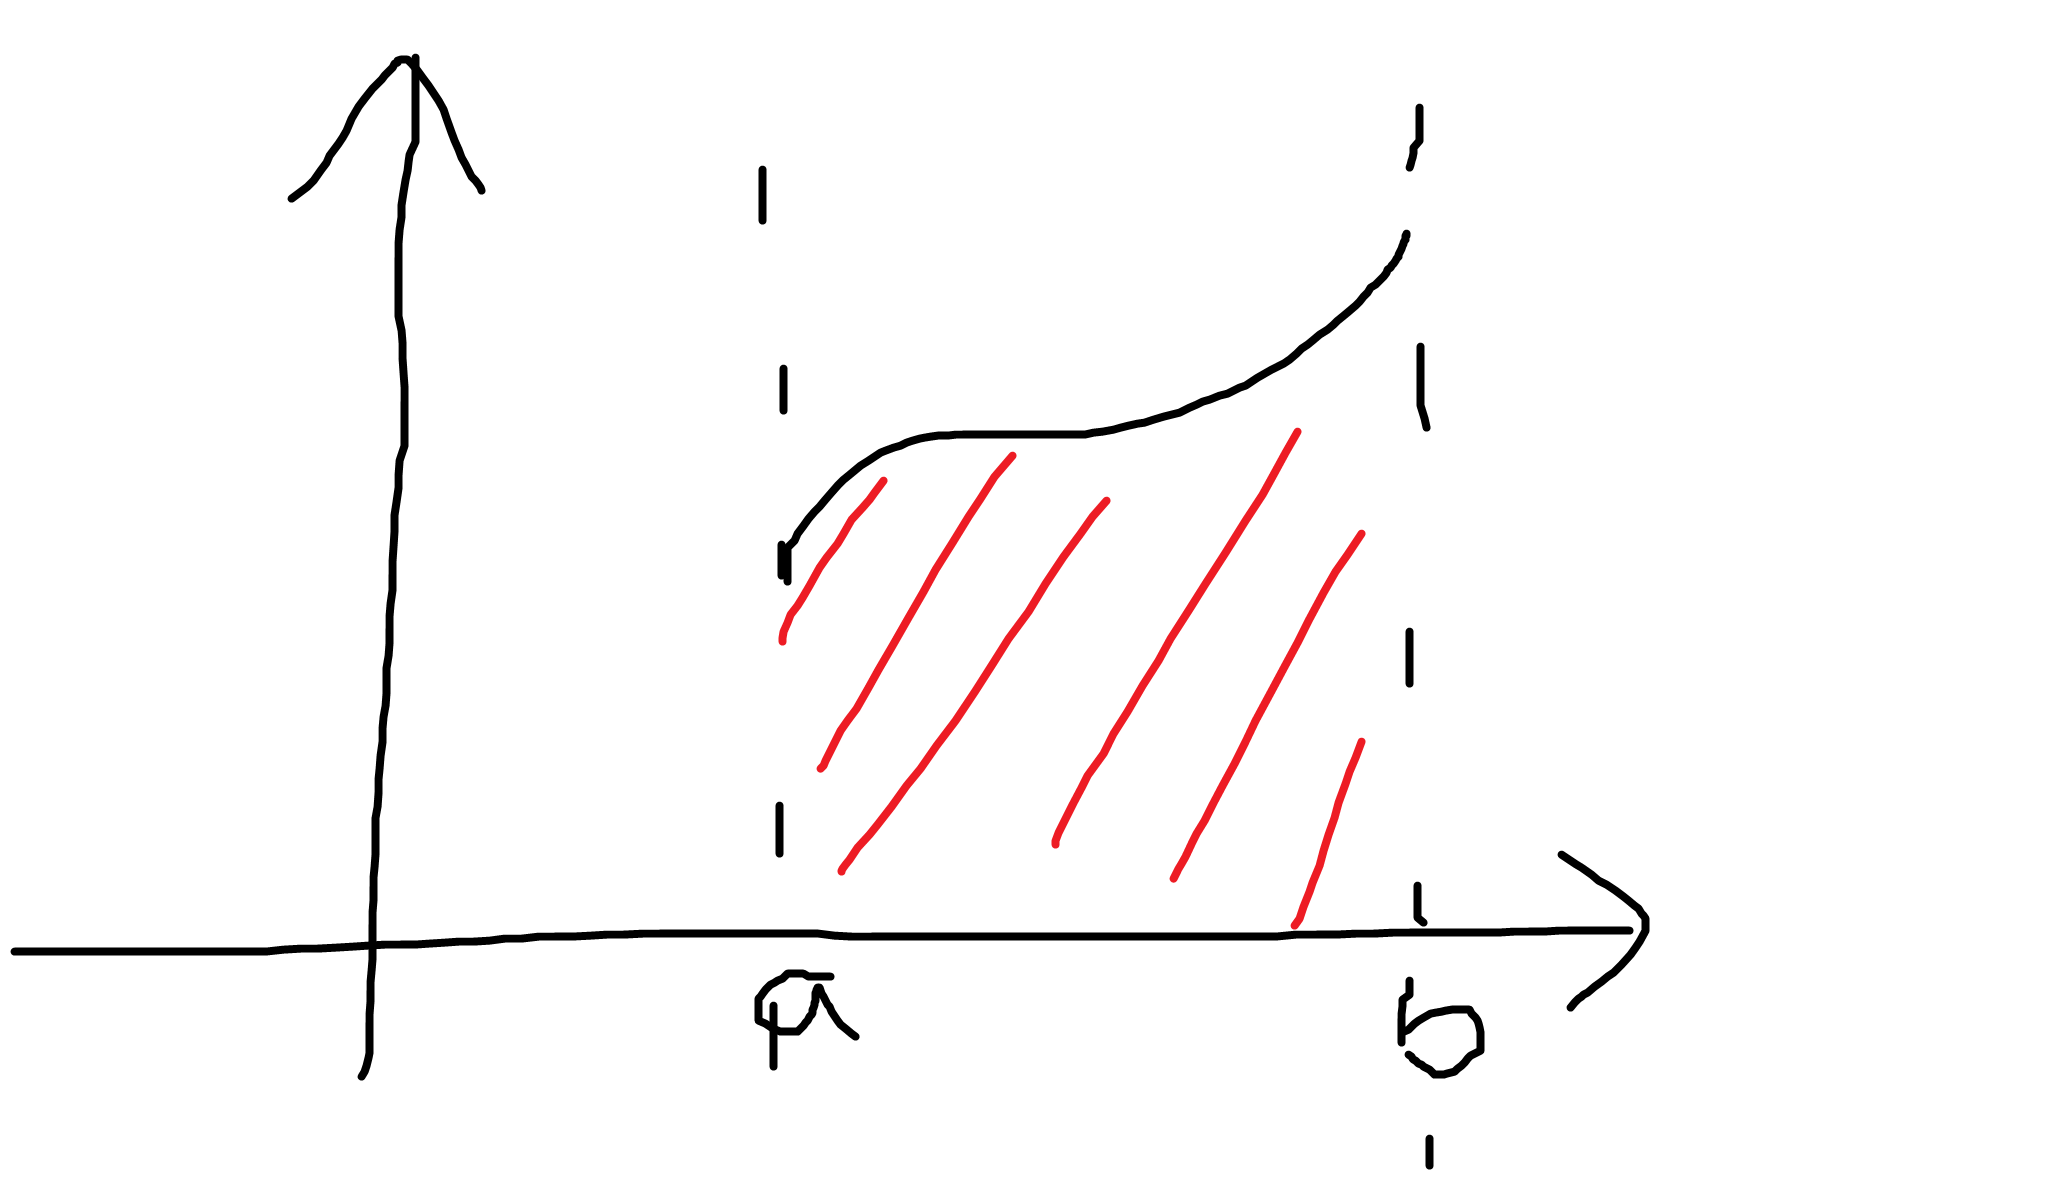
\includegraphics[height=3cm]{kepek/01.png}
			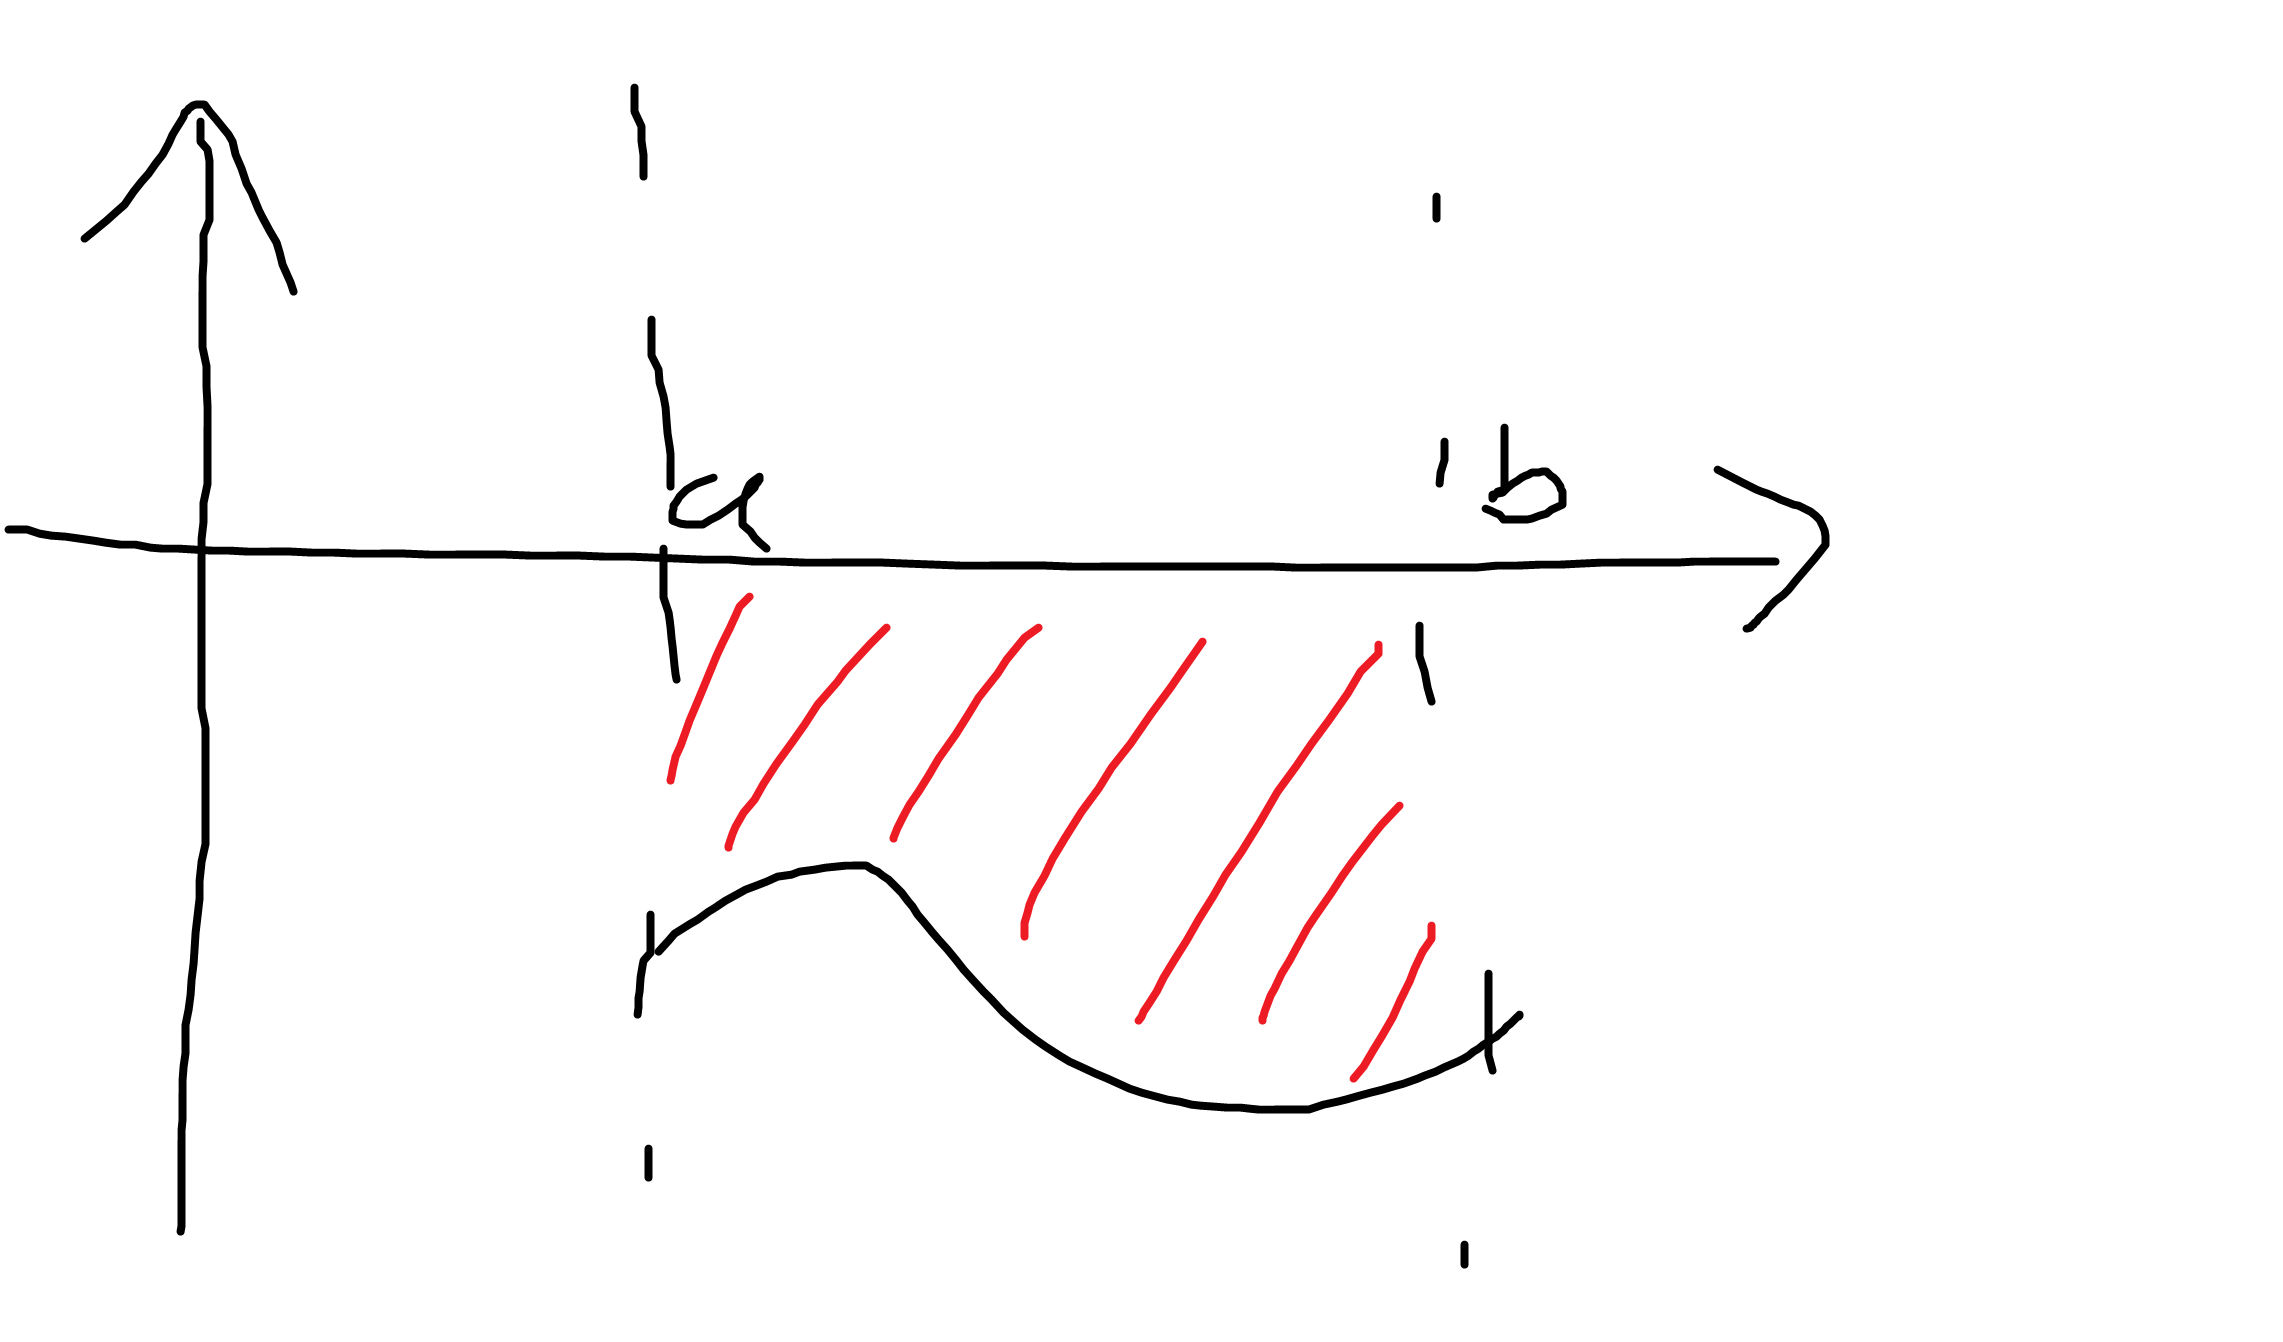
\includegraphics[height=3cm]{kepek/02.png}
			\caption{Rendre: $T=\int_a^bf,\quad f>0$,\quad valamint\quad  $T=\int_a^bf,\quad f<0$}
		\end{figure}
		\begin{figure}[H]
			\centering
			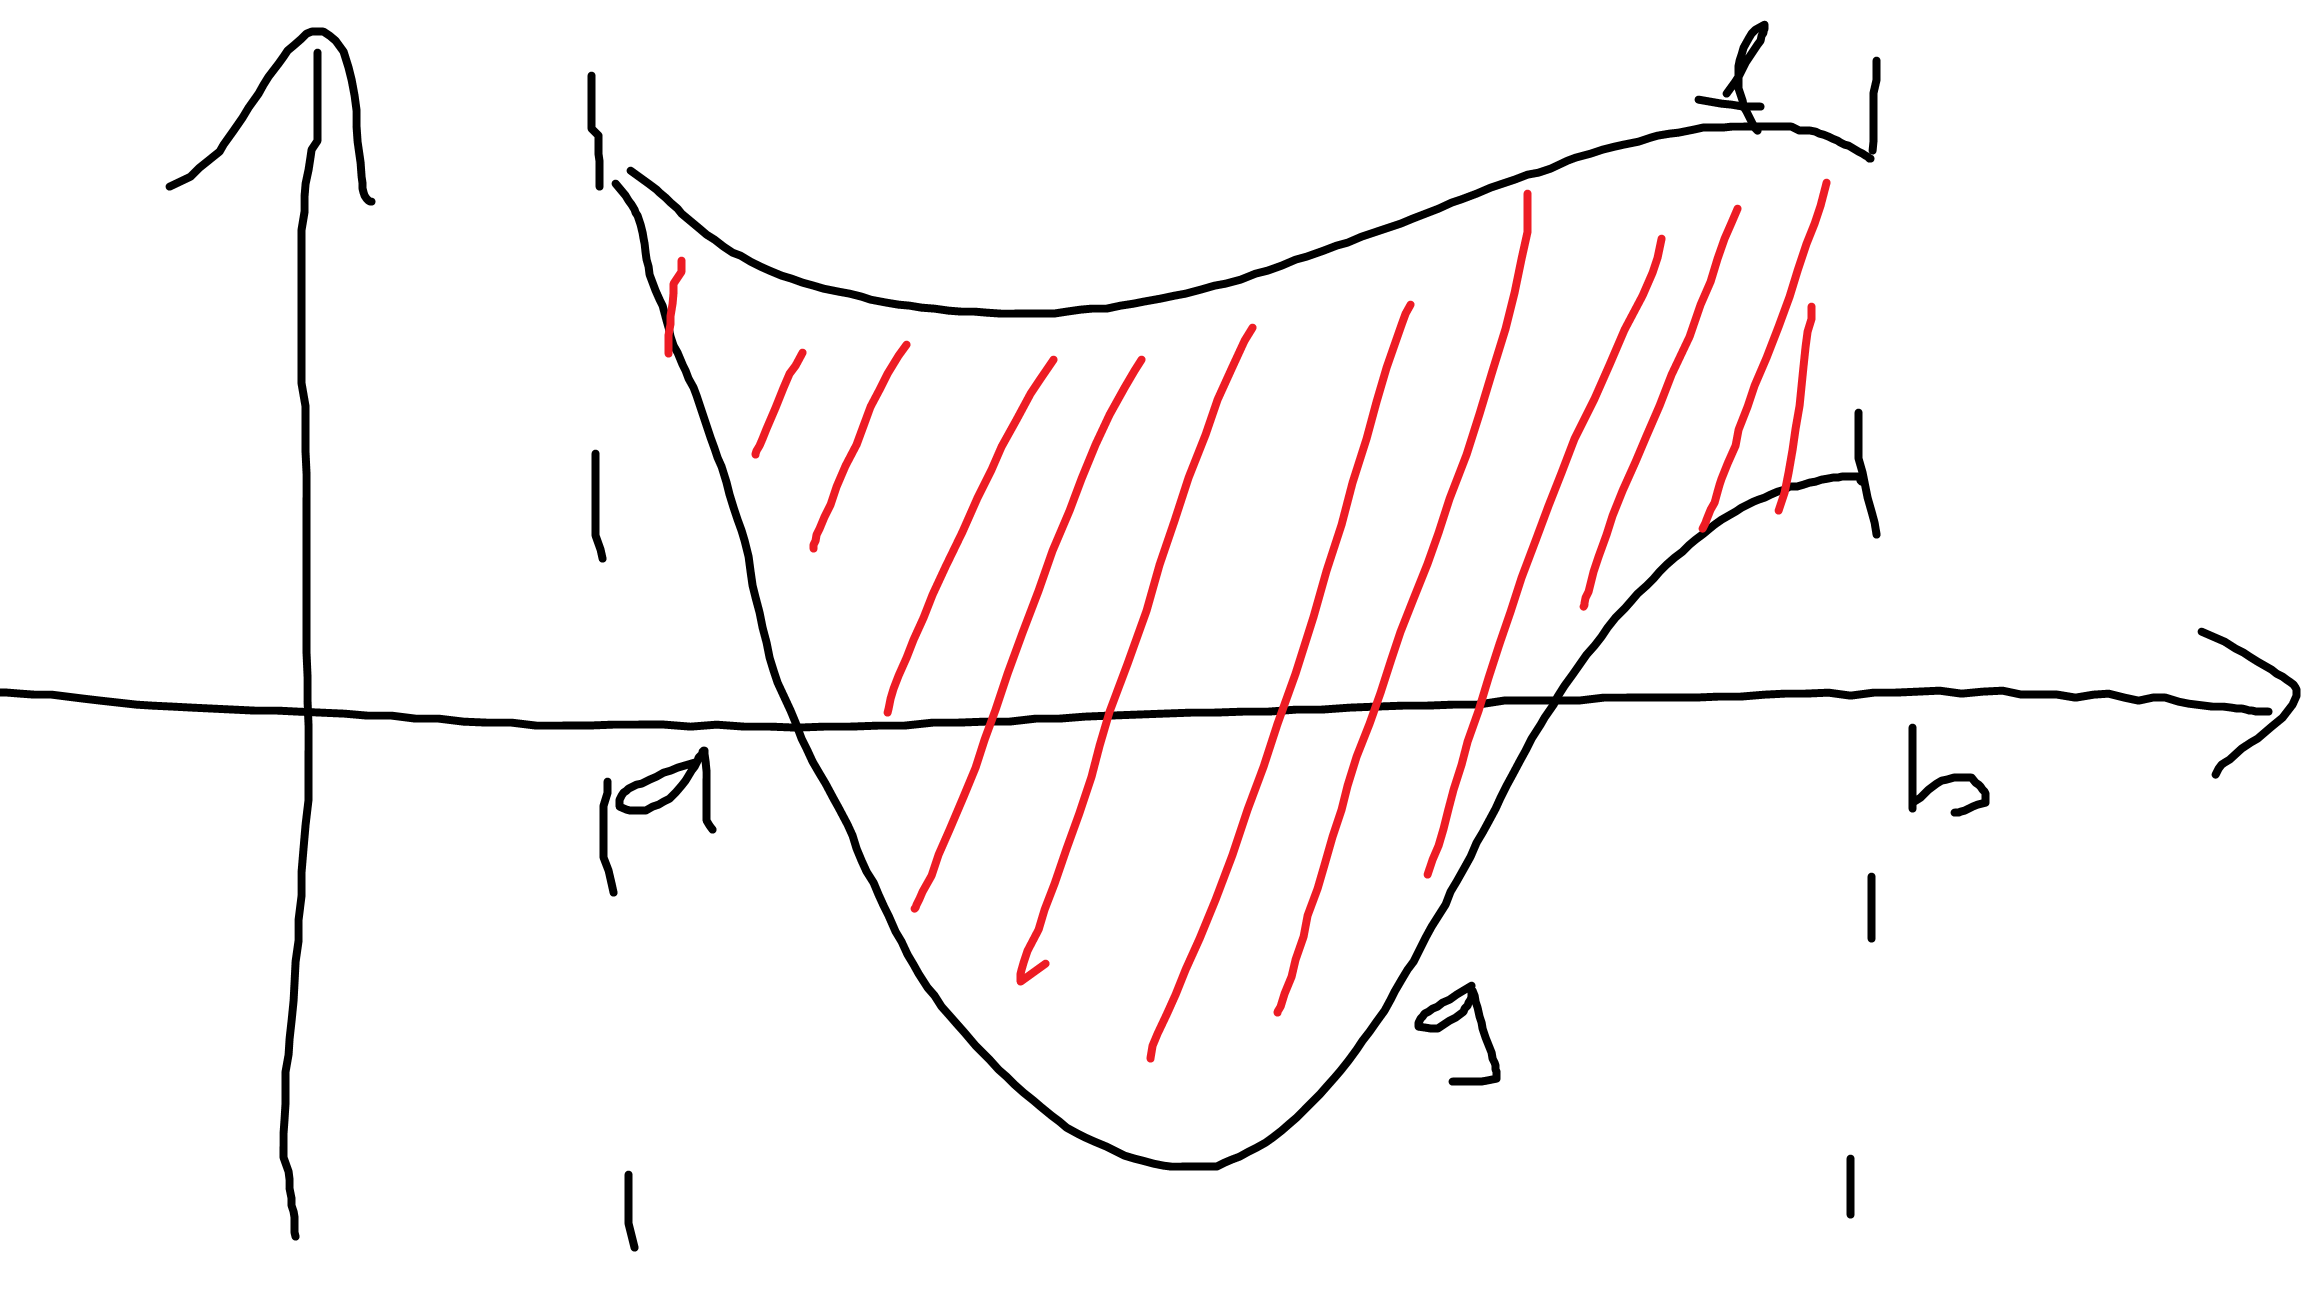
\includegraphics[height=3cm]{kepek/03.png}
			\caption{}\label{eltolatlan-fv}
		\end{figure}
		Hogyan lehet megoldani ezt? Megoldás: eltoljuk a függvényt.
		\begin{figure}[H]
			\centering
			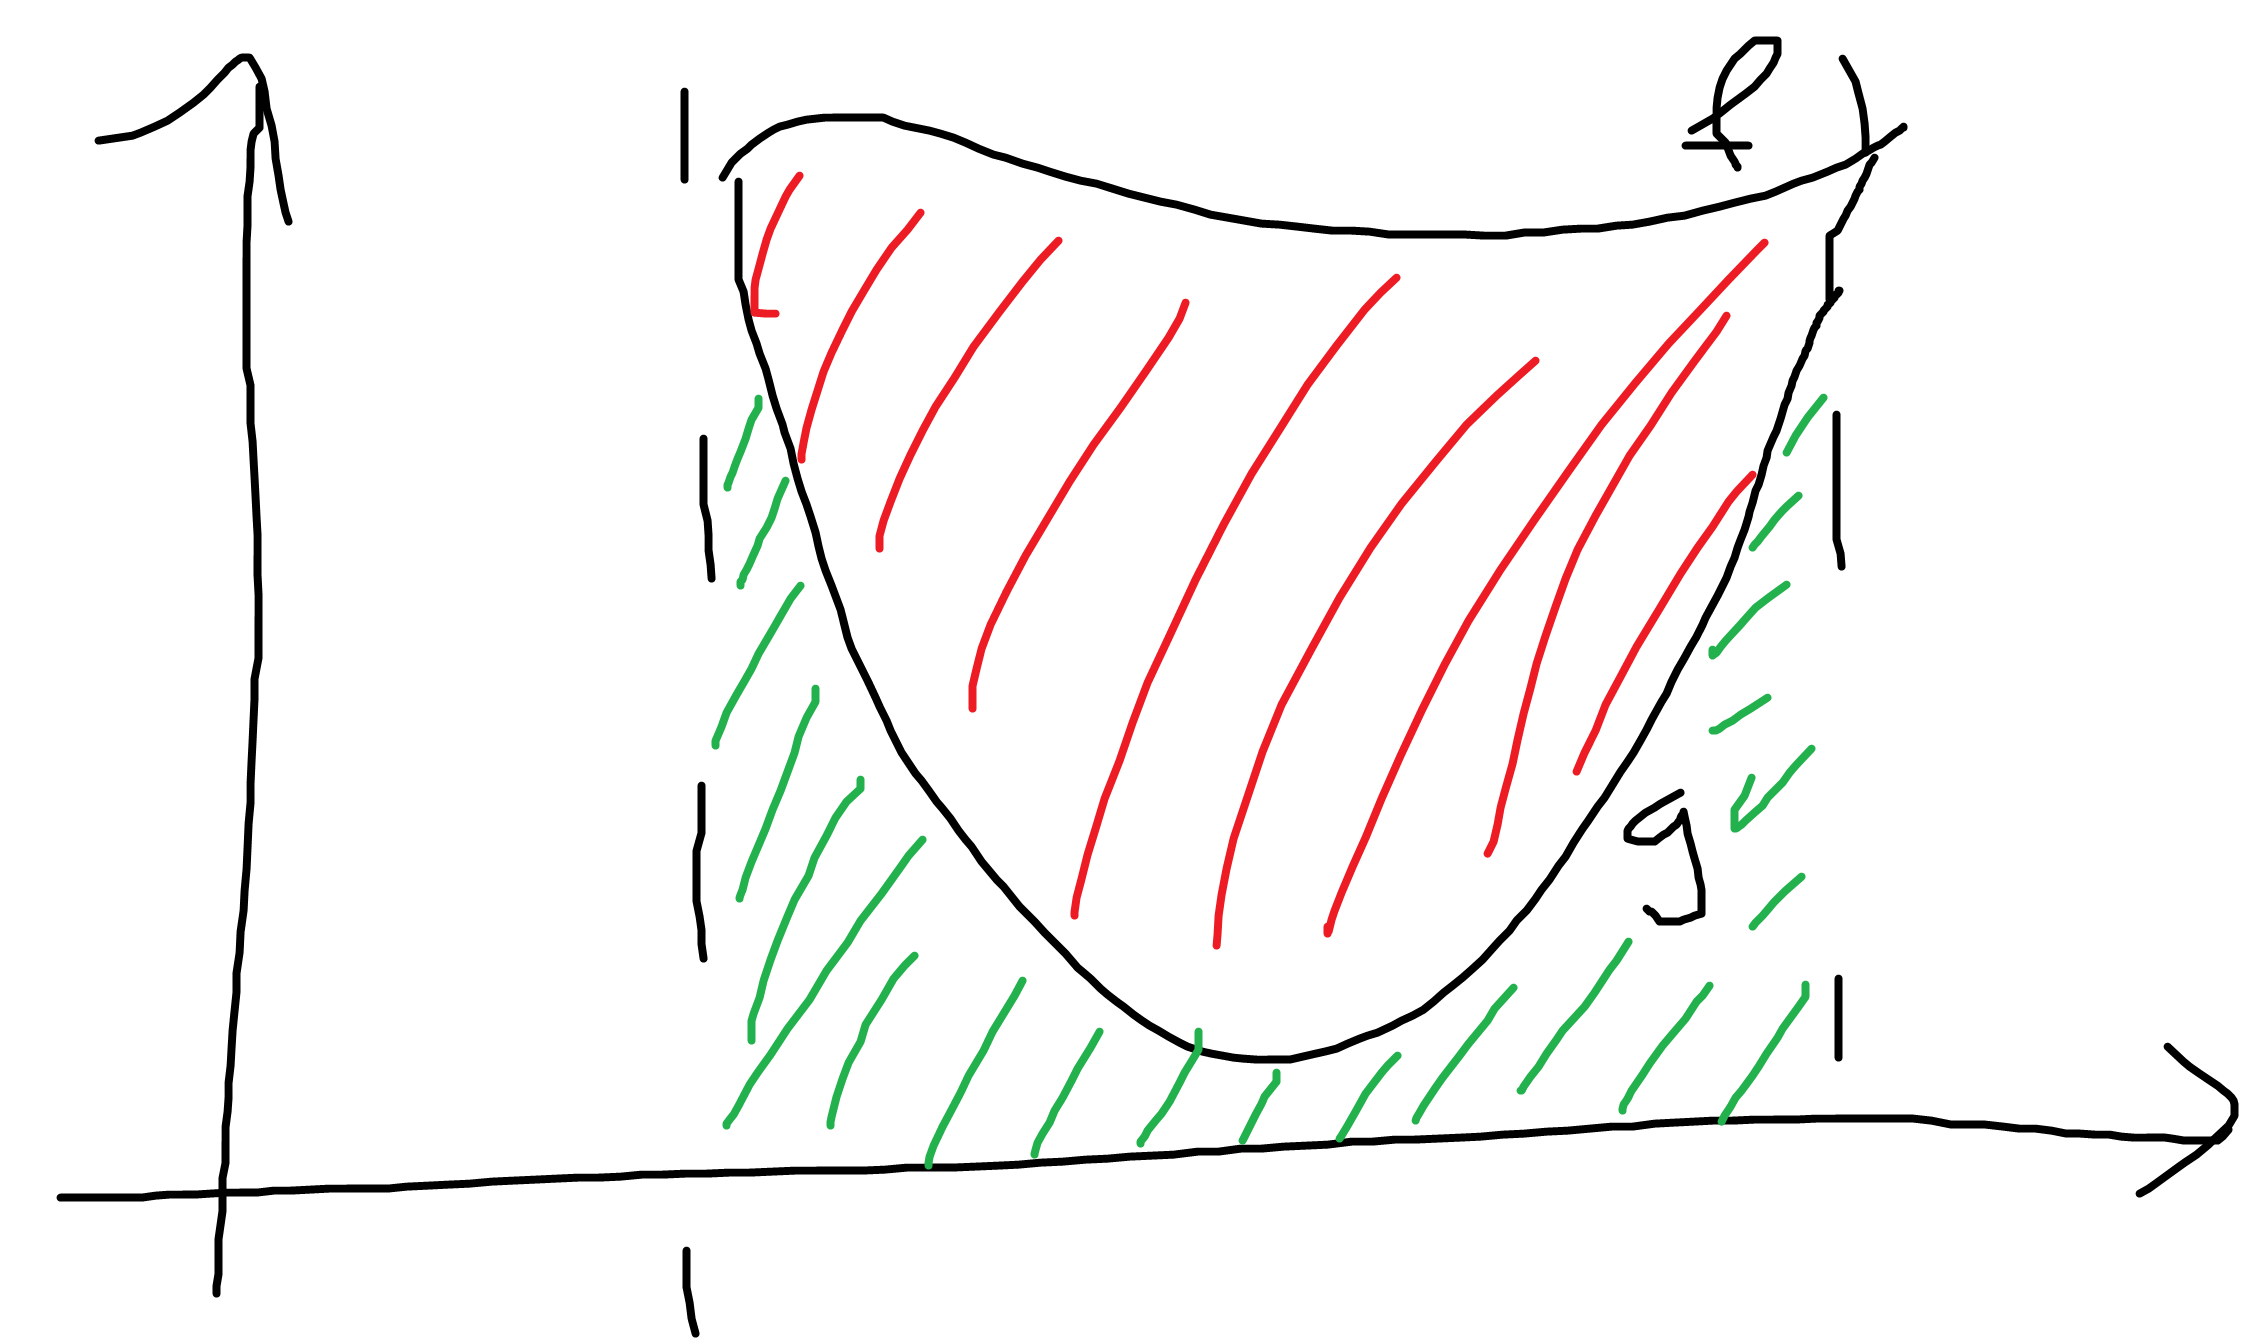
\includegraphics[height=2cm]{kepek/04.png}
			\caption{Ugyanaz az mint a \ref{eltolatlan-fv}. ábra, adott $c$ konstanssal eltolva.}
		\end{figure}
		Így már a terület könnyen meghatározható:
		\[ T=\int_a^b(f+c)-\int_a^b(g+c)=\int_a^b(f-g) \]
		\begin{figure}[H]
			\centering
			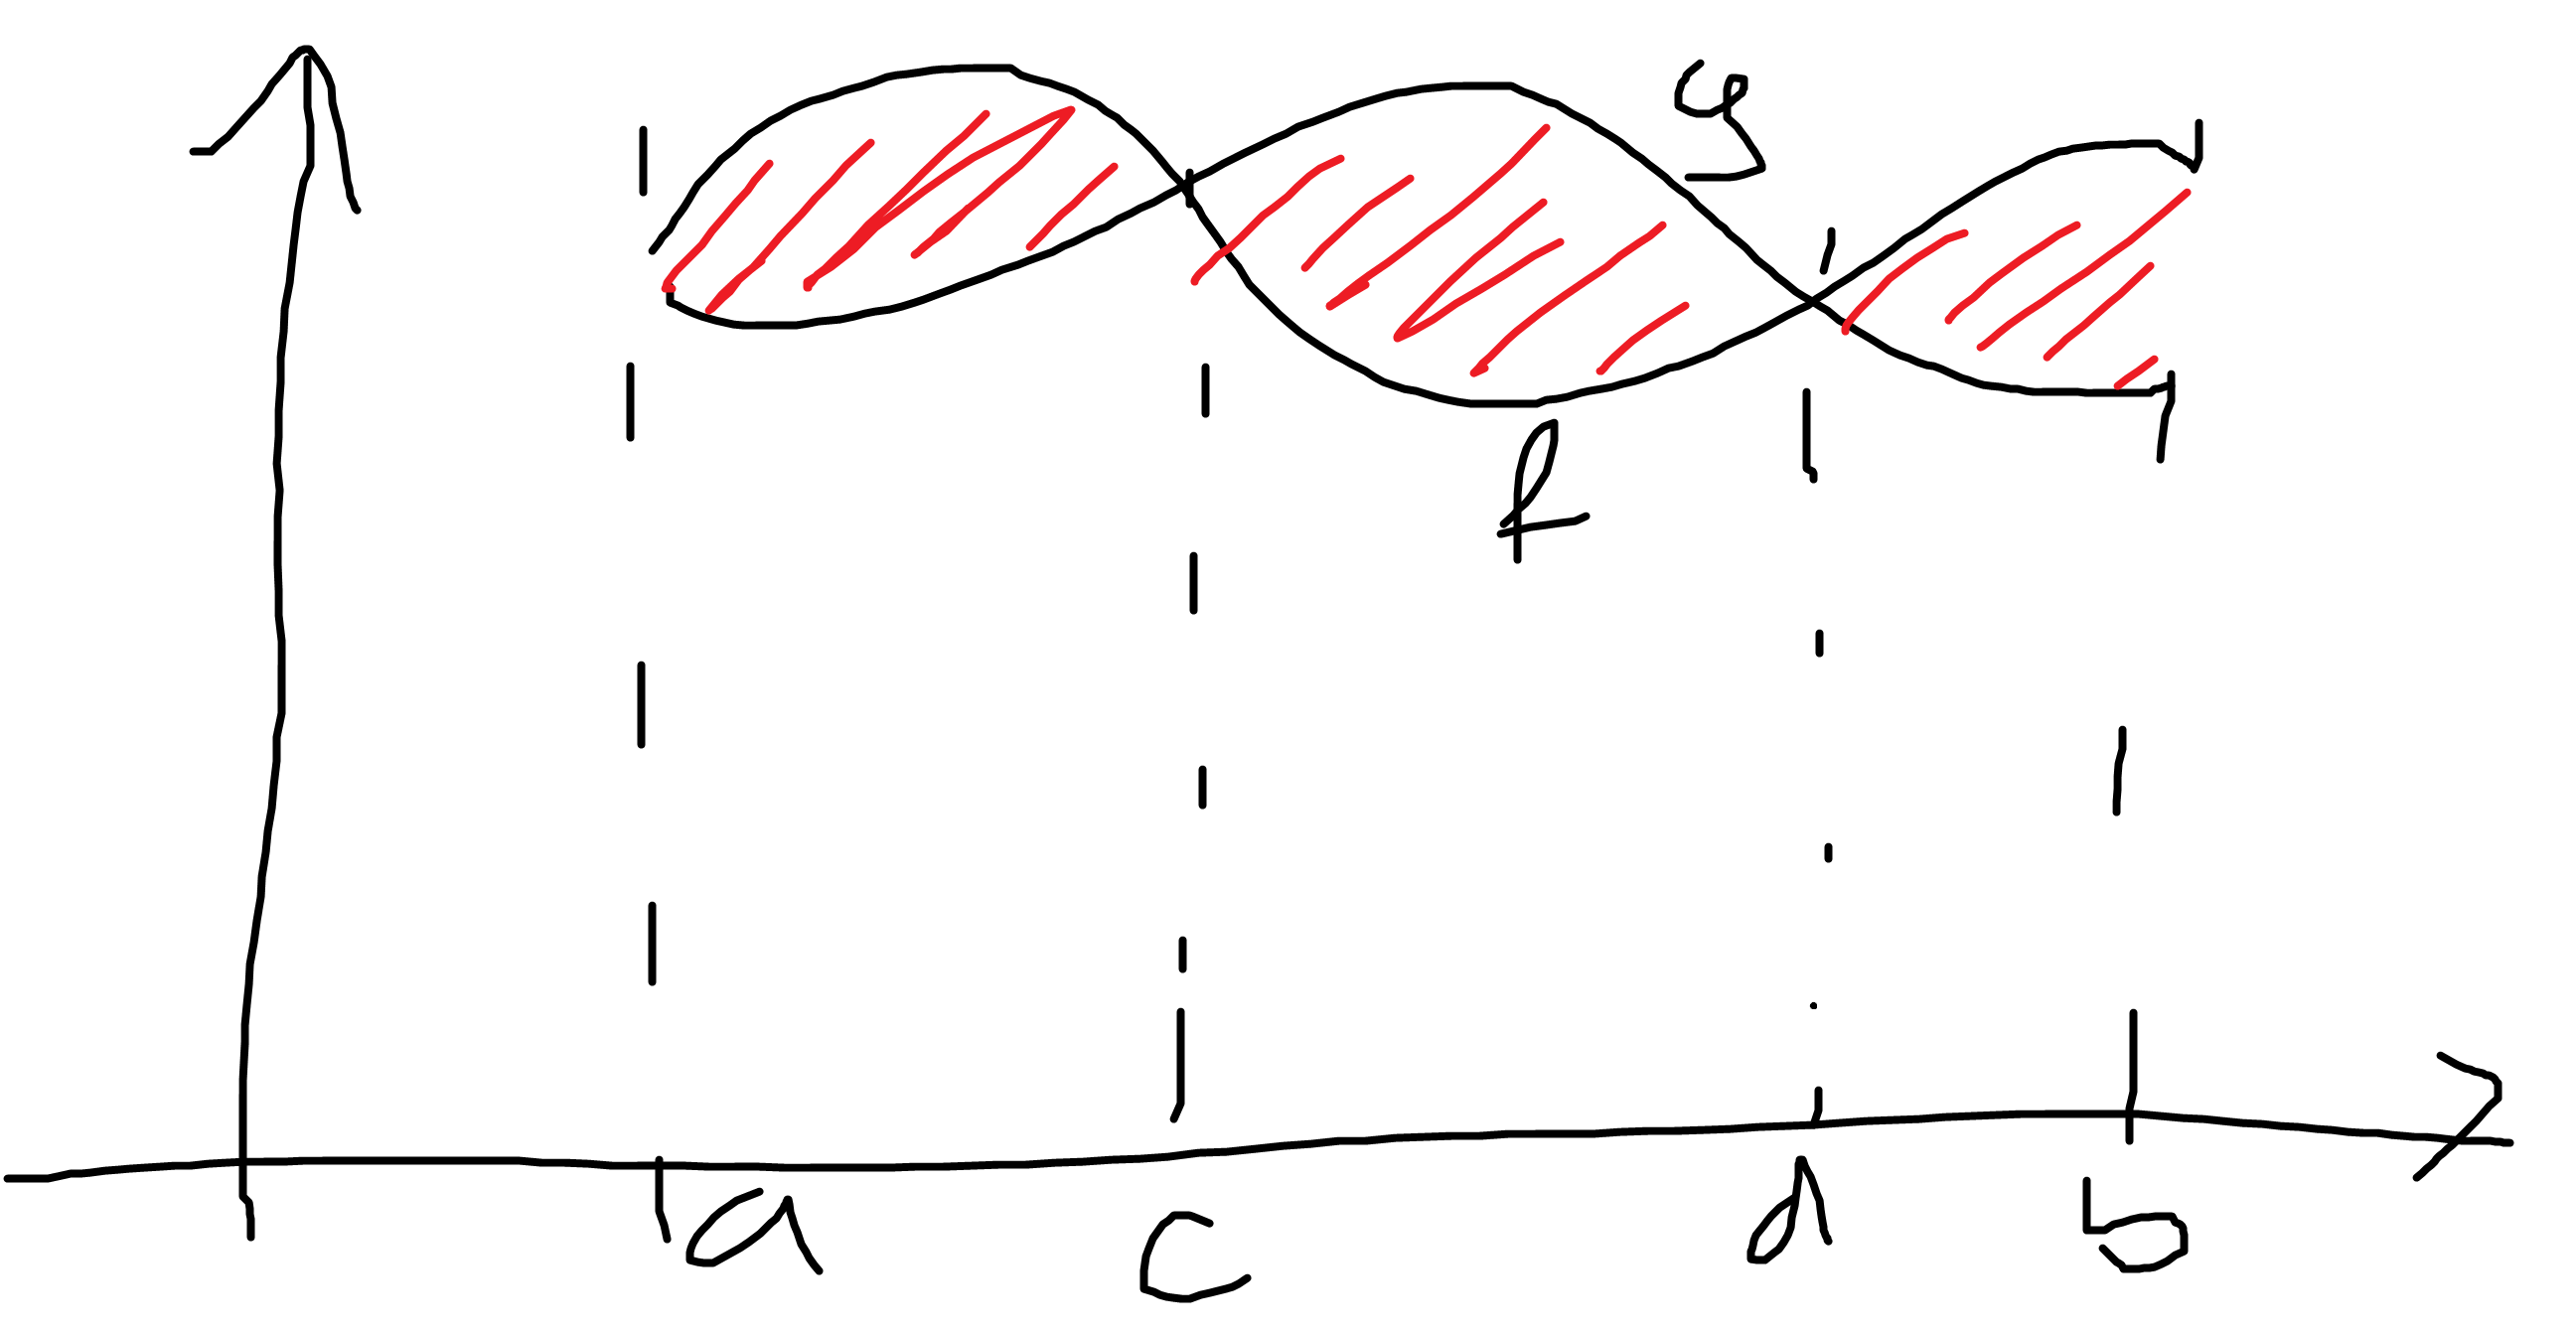
\includegraphics[height=3cm]{kepek/05.png}
			\caption{}
		\end{figure}
		\[ T=\int_a^c(f-g)+\int_c^d(g-f)+\int_d^b(f-g)=\int_a^b|f-g|= \]
		Megállapítható, hogy ez $f$ és $g$ 1-es metrikája.
		\[ =\rho_1(f,g),\quad (f,g\in C[a,b]) \]
		
		Szimmetriák kihasználása:
		\begin{figure}[H]
			\centering
			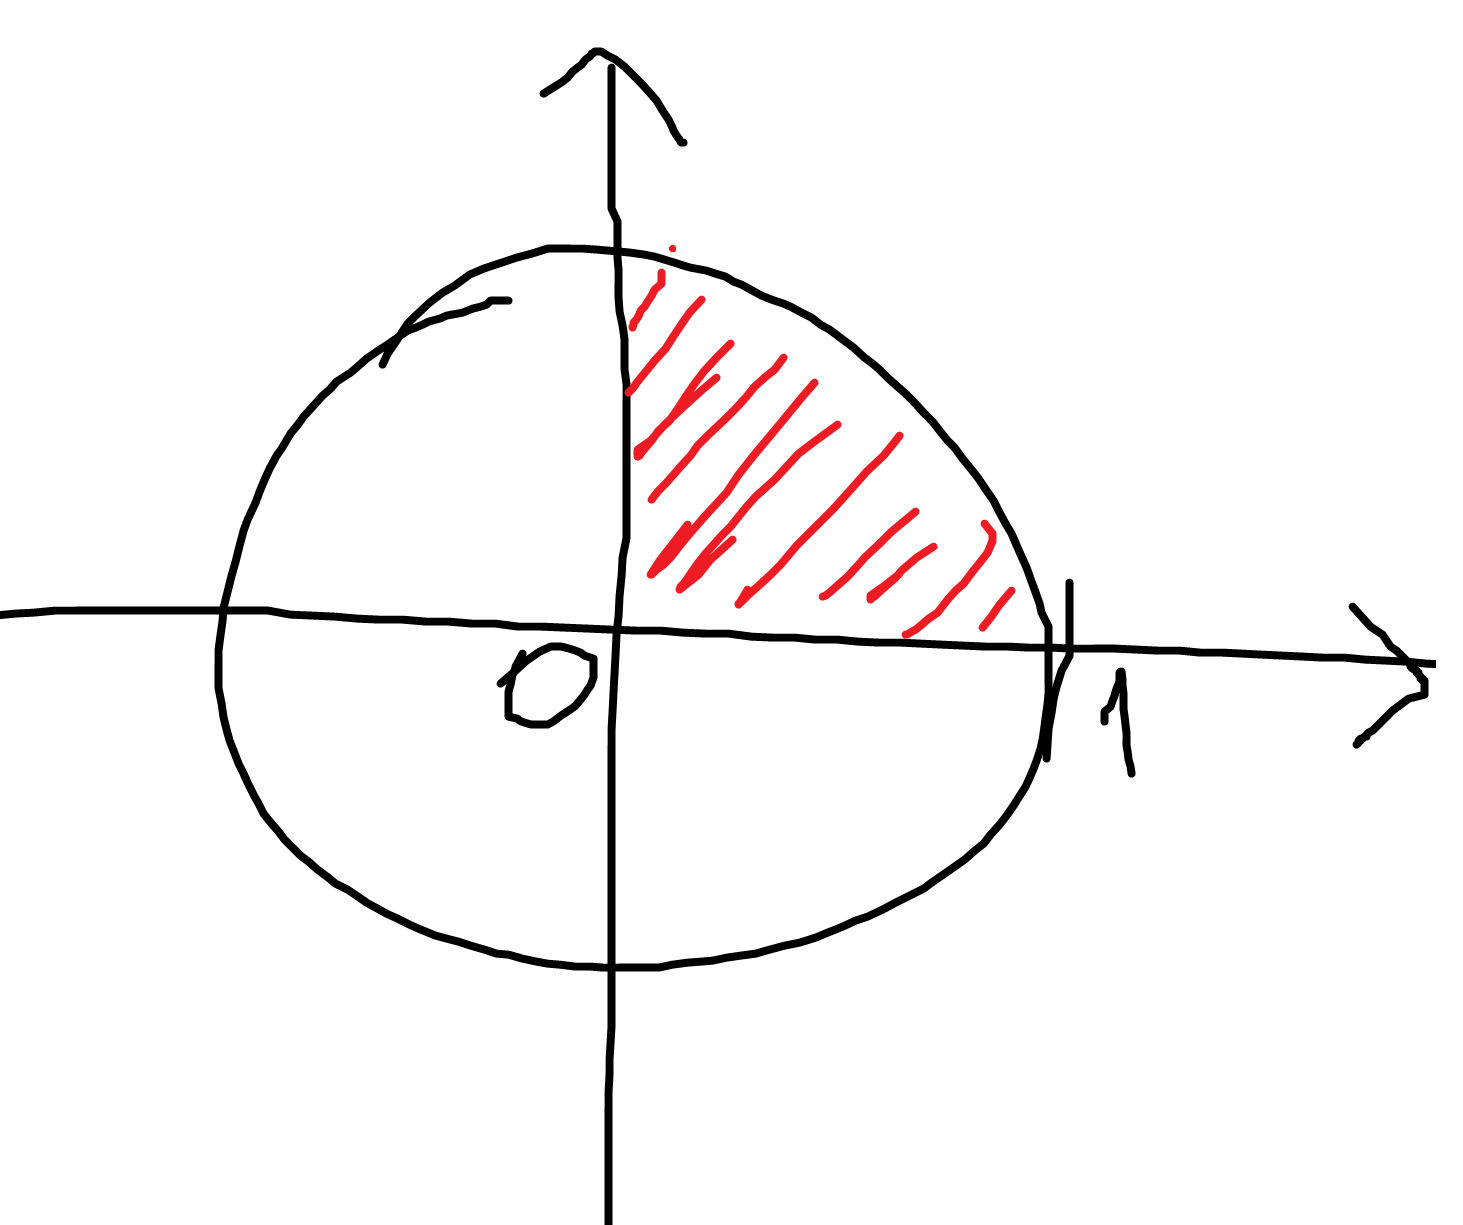
\includegraphics[height=3cm]{kepek/06.png}
			\caption{Elég a negyed kör területének meghatározása.}
		\end{figure}
		\[ T_{\text{kör}}=4\cdot T_{\text{negyedkör}}=4\cdot\int_0^1\sqrt{1-x^2}\,dx \]
		Szimmetria kihasználható így is:
		\begin{figure}[H]
			\centering
			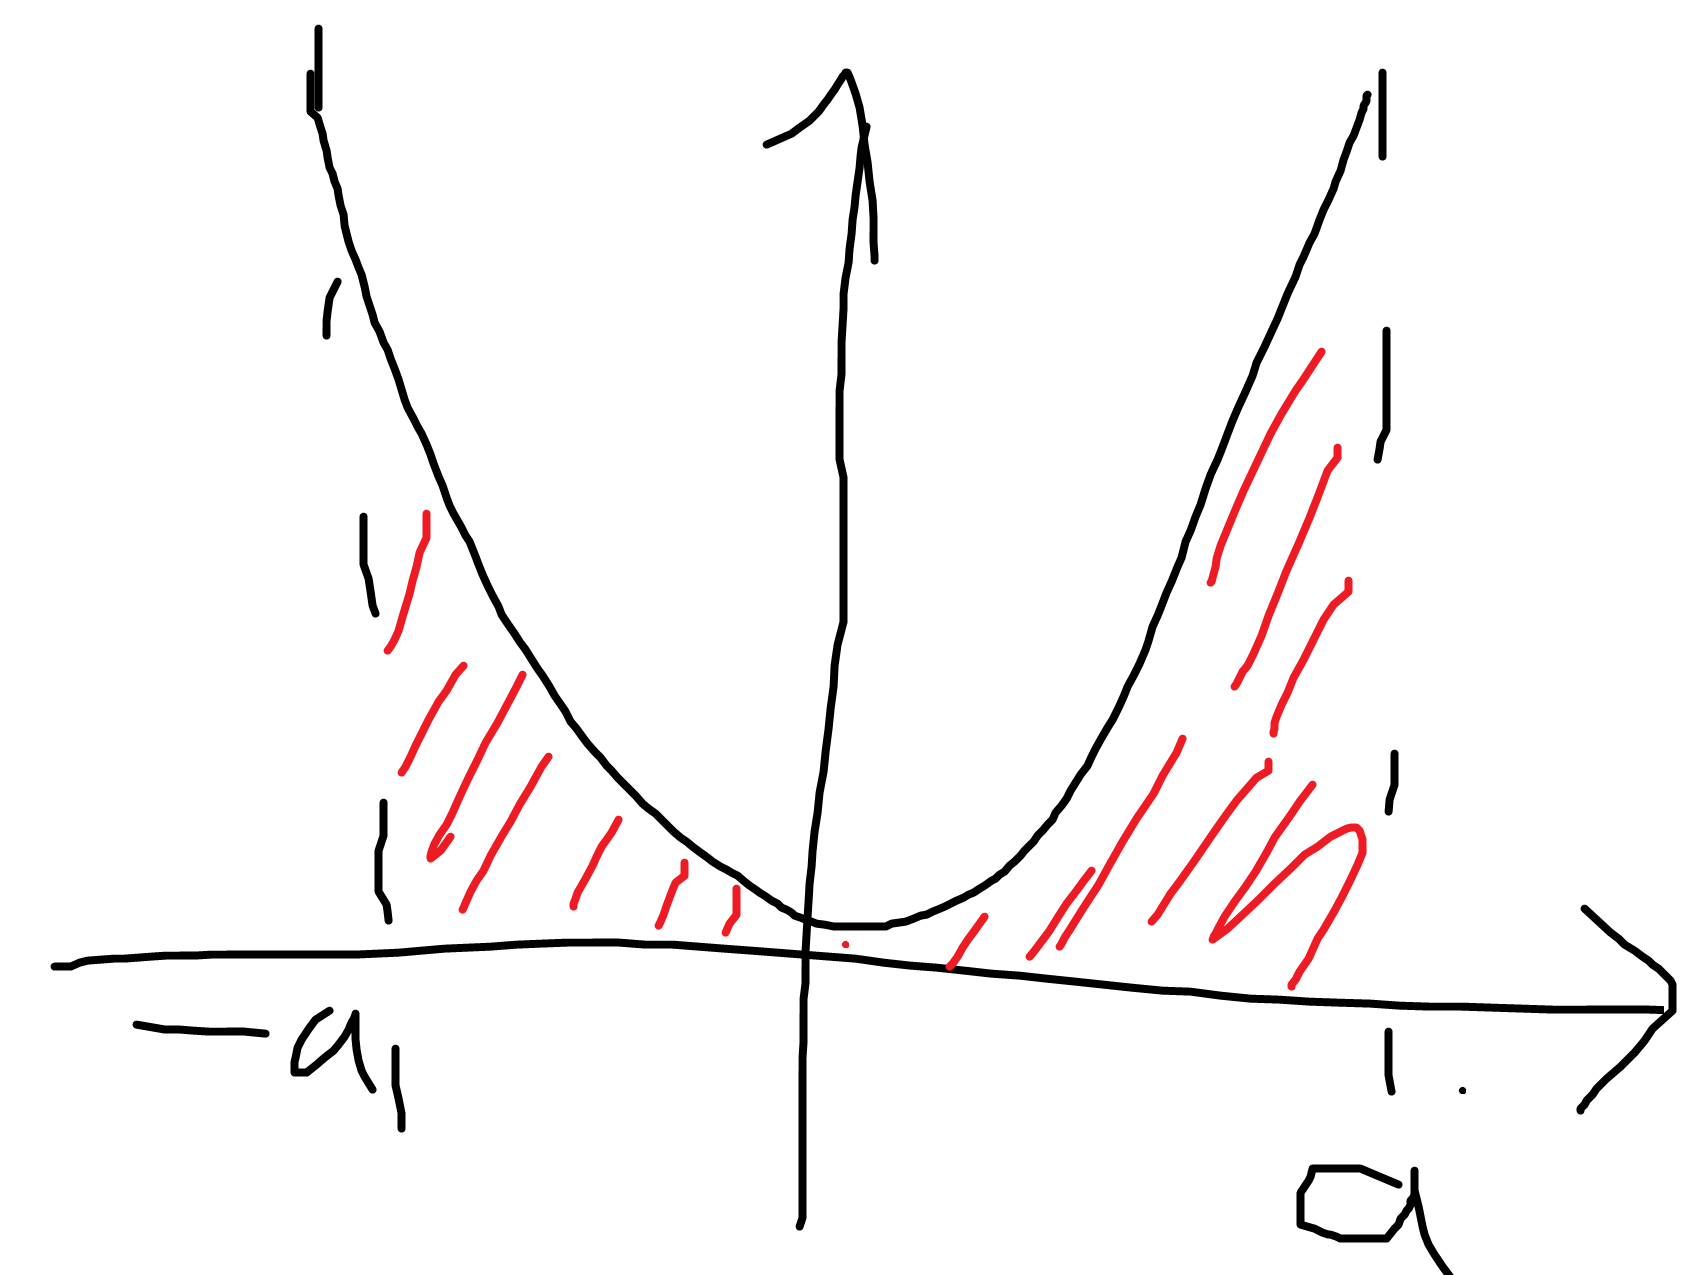
\includegraphics[height=3cm]{kepek/07.png}
			\caption{Elegendő a $[0,a]$ intervallumon a függvény integráltjának kétszeresét meghatározni.}
		\end{figure}
		\[ \int_{-a}^{a}f=2\cdot\int_0^af \]
		Megállapítható és kihasználható, hogy $f(x):=x^2$ páros.
		
		
	\begin{revision}
		Newton-Leibniz tétel: Ha $f\in\R[a,b]$ és $\int f\not=0$ 
			\[ \int_a^bf(x)\,dx=F(b)-F(a)=:[F(x)]_a^b\quad (\forall F\in\int f) \]
	\end{revision}
	\begin{example}
		Mennyi az e két \textit{reláció} által határolt terület?
			
		\[\begin{cases}
			y=x-1\\
			y^2=2x+6
		\end{cases}\]
		Világos, hogy a másik \textit{reláció} nem \textit{függvény}, azonban fel tudjuk írni két függvény együtteseként.
		\[y^2=2x+6\Leftrightarrow\quad y=\pm\sqrt{2x+6}\quad \Leftrightarrow\quad x=\frac{y^2-6}{2} \]
		\begin{figure}[H]
			\centering
			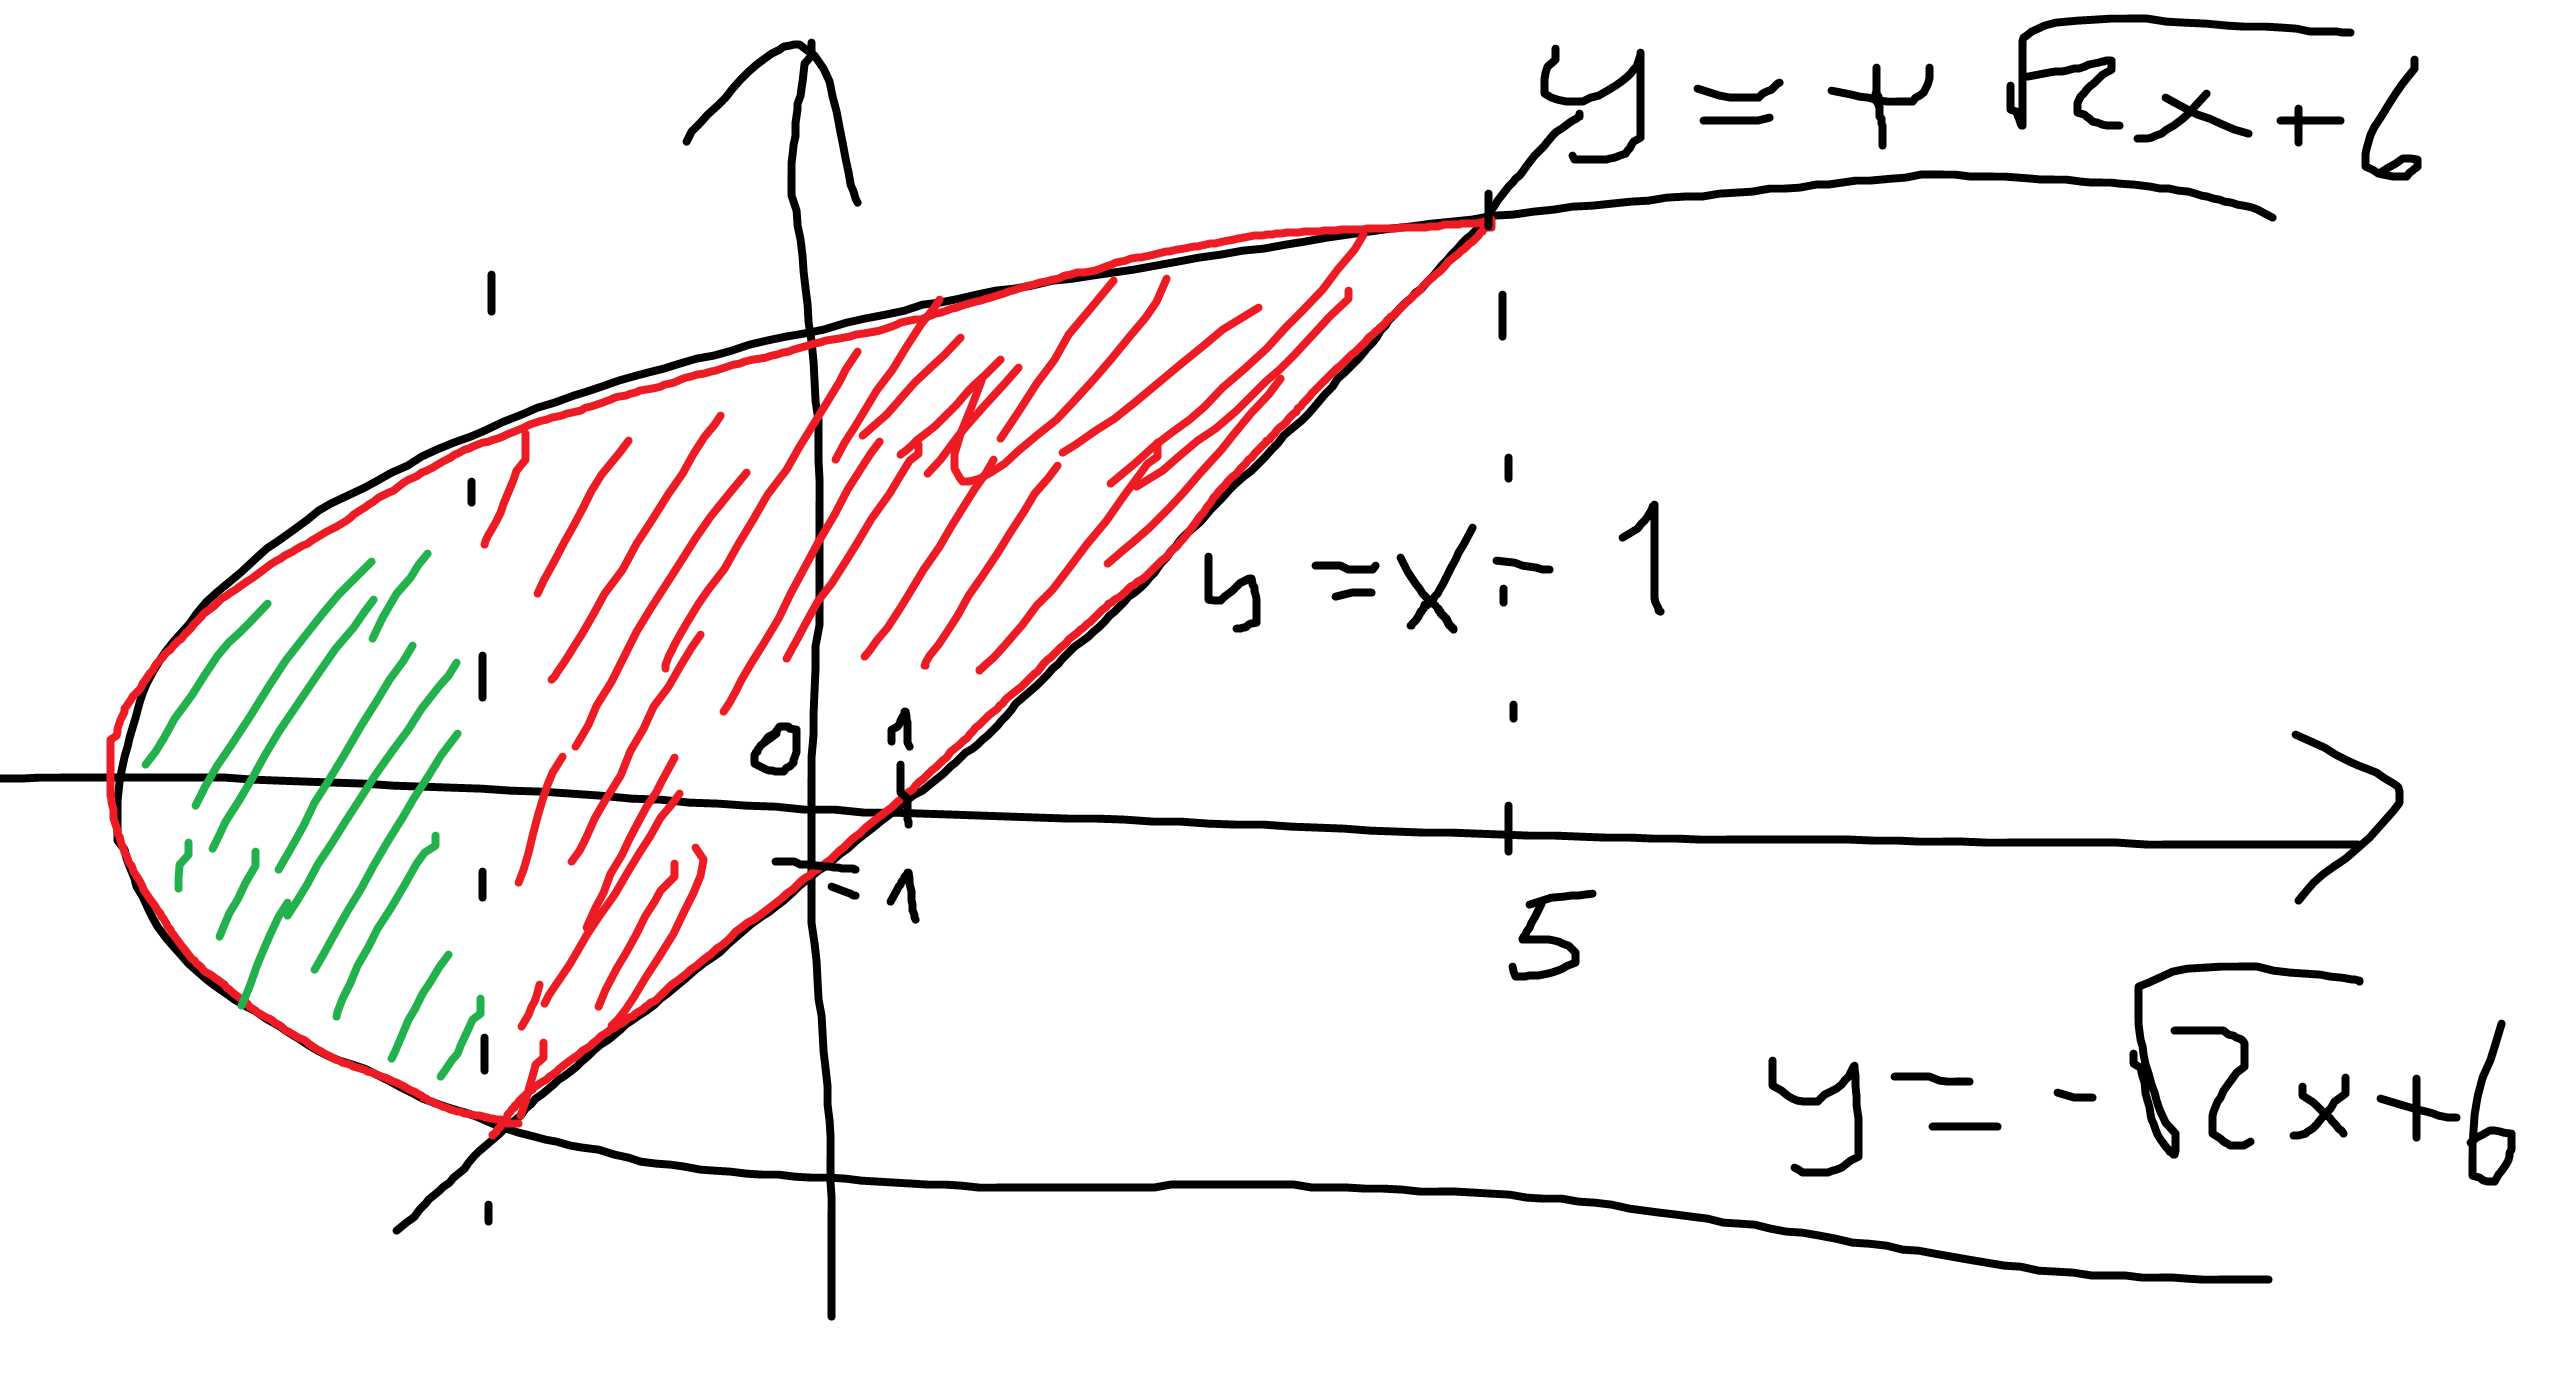
\includegraphics[height=3cm]{kepek/08.png}
			\caption{}
		\end{figure}
		Most már megállapítható a függvények metszéspontjai:
		\[ (x-1)^2=2x+6\quad \Leftrightarrow\quad x_1=-1\quad \text{és\quad } x_2=5 \]
		Valamint megállapítható, hogy az $y=\pm\sqrt{2x-6}$ függvények a $-3$ pontban metszik az $x$ tengelyt.
		\smallskip
		
		Ez alapján a területet kiszámolhatjuk. A zöld területről megállapítható hogy szimmetrikus, és ezt ki is használhatjuk.
		\[ T=2\cdot\int_{-3}^{-1}\sqrt{2x+6}\,dx+\int_{-1}^{5}\left(\sqrt{2x+6}-(x-1)\right)\,dx=2\cdot\left[\frac{(2x+6)^{\frac{3}{2}}}{\frac{3}{2}\cdot2}\right]_{-3}^{-1}+\left[\frac{(2x+6)^{\frac{3}{2}}}{\frac{3}{2}\cdot2}-\frac{x^2}{2}+x\right]^{5}_{-1}=\]
		\[=\frac{2}{3}\left[4^\frac{3}{2}-0\frac{3}{2}\right]+\frac{16^\frac{3}{2}}{3}-\frac{25}{2}+5-\left(\frac{4^\frac{3}{2}}{3}-\frac{1}{2}-1\right)=18  \]
	\end{example}
	\begin{example}Határozzuk meg az ezen görbék által határolt területet!
		\[\begin{cases}
			y=x^3\\
			y^2+x^2=2\\
			y=0
		\end{cases}\]
		\begin{figure}[H]
			\centering
			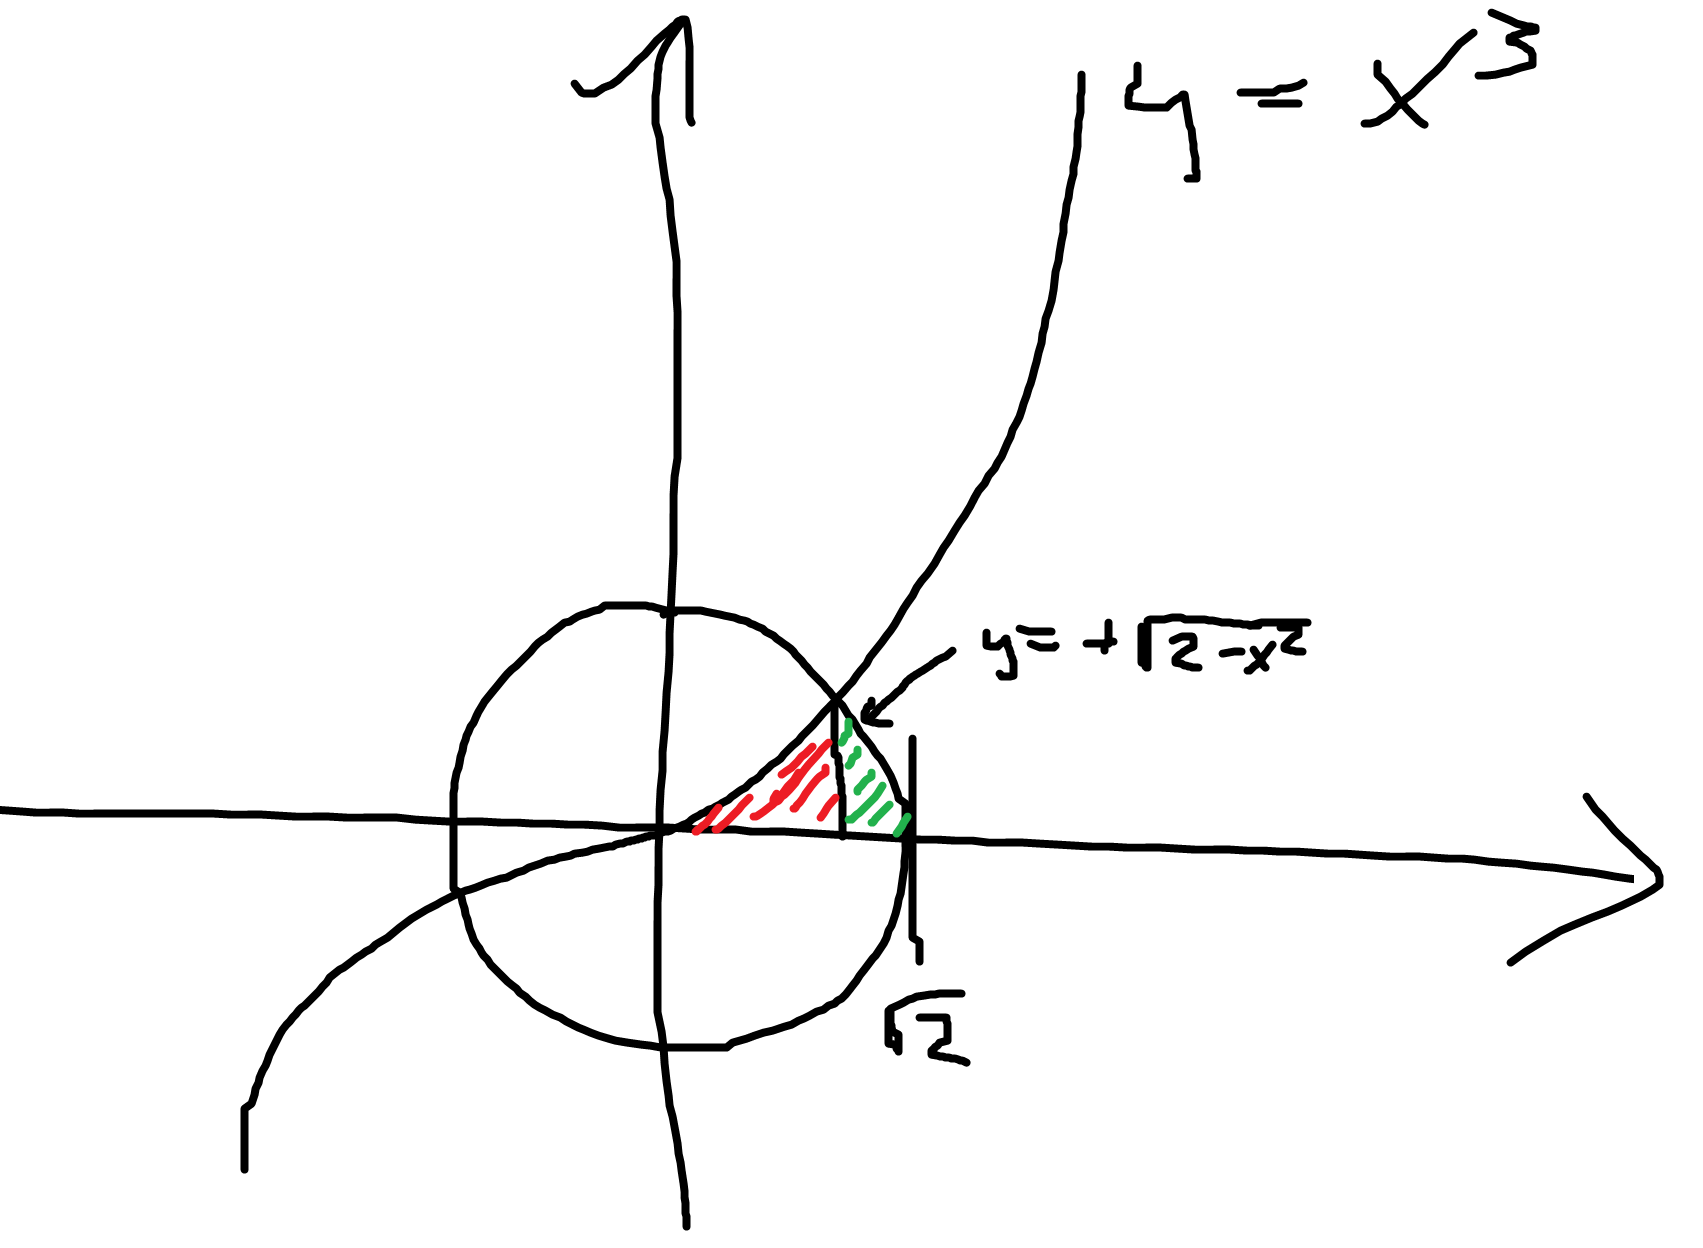
\includegraphics[height=4cm]{kepek/09.png}
			\caption{}
		\end{figure}
		Metszéspontok: (megfigyelhető, hogy az első egyenletet négyzetre emeltük)
		\begin{align*}
			x^2+x^6-2=0\\
			x^6-1+x^2-1=0\\
		\end{align*}
		Külön megállapítandó:
		\[(x^2-1)(x^4+x^2+1)=0\quad \Rightarrow\quad x=\pm1 \]
		\[ x^2-1=0\quad \Rightarrow\quad x=\pm1 \]
		Számoljuk ki  területet. A körre természetes okokból nem tudunk függvényt felírni, azonban megállapítható, hogy a számunkra fontos körnegyed egyenlete $y=+\sqrt{2-x^2}$.
		\[ T=\int_0^1x^3\,dx+\int_1^{\sqrt{2}}\sqrt{2-x^2}\,dx=\left[\frac{x^4}{4}\right]_0^1+I=\frac{1}{4}+I \]
		Ahol:
		\[ I=\int_1^{\sqrt{2}}\sqrt{2-x^2}\,dx=\sqrt{2}\cdot\int_1^{\sqrt{2}}\sqrt{1-\left(\frac{x}{\sqrt{2}}\right)^2}\,dx= \]
		Vezessünk be egy új változót.
		\[ \sin t:=\frac{x}{\sqrt{2}},\quad t=\arc\sin\left(\frac{x}{\sqrt{2}}\right) \]
		\[\text{Ha}\quad x=1\quad \Rightarrow\quad t=\arc\sin\frac{1}{\sqrt{2}}=\arc\sin\frac{\sqrt{2}}{2}=\frac{\pi}{4} \]
		\[\text{Ha}\quad x=\sqrt{2}\quad \Rightarrow\quad t=\arc\sin1=\frac{\pi}{2} \]
		Visszatérve:
		\[ =\sqrt{2}\cdot\int_{\frac{\pi}{4}}^{\frac{\pi}{2}}\sqrt{1-\sin^2t}\cdot\sqrt{2}\cos t\,dt= \]
		Visszahelyettesíteni fölösleges, hisz nem primitív függvényt, hanem egy konkrét számot keresünk.
		\[ =2\cdot\int_{\frac{\pi}{4}}^{\frac{\pi}{2}}|\cos t|\cdot\cos t\,dt\quad \overset{\frac{\pi}{4}\leq t\leq \frac{\pi}{2}}{=}\quad2\cdot\int_{\frac{\pi}{4}}^{\frac{\pi}{2}}\overbrace{\cos^2t}^{\frac{1+\cos2t}{2}}\,dt=\left[t+\frac{\sin2t}{2}\right]_{\frac{\pi}{4}}^{\frac{\pi}{2}}=\frac{\pi}{2}+\frac{\sin\pi}{2}-\frac{\pi}{4}-\frac{\sin\frac{\pi}{2}}{2}=\frac{\pi}{4}-\frac{1}{2}  \]
	\end{example}
	\begin{note}
		Okkal $I$-vel, és nem $I(x)$-el jelölünk. A határozatlan integrál egy függvény, a határozott csupán egy szám.
	\end{note}
	\begin{example}
		Számítsuk ki a következő minimumot:
		\[ \min\left\{\int _0^1|x^2-c|\,dx\quad :\quad c\in\R \right\} \]
		\begin{figure}[H]
			\centering
			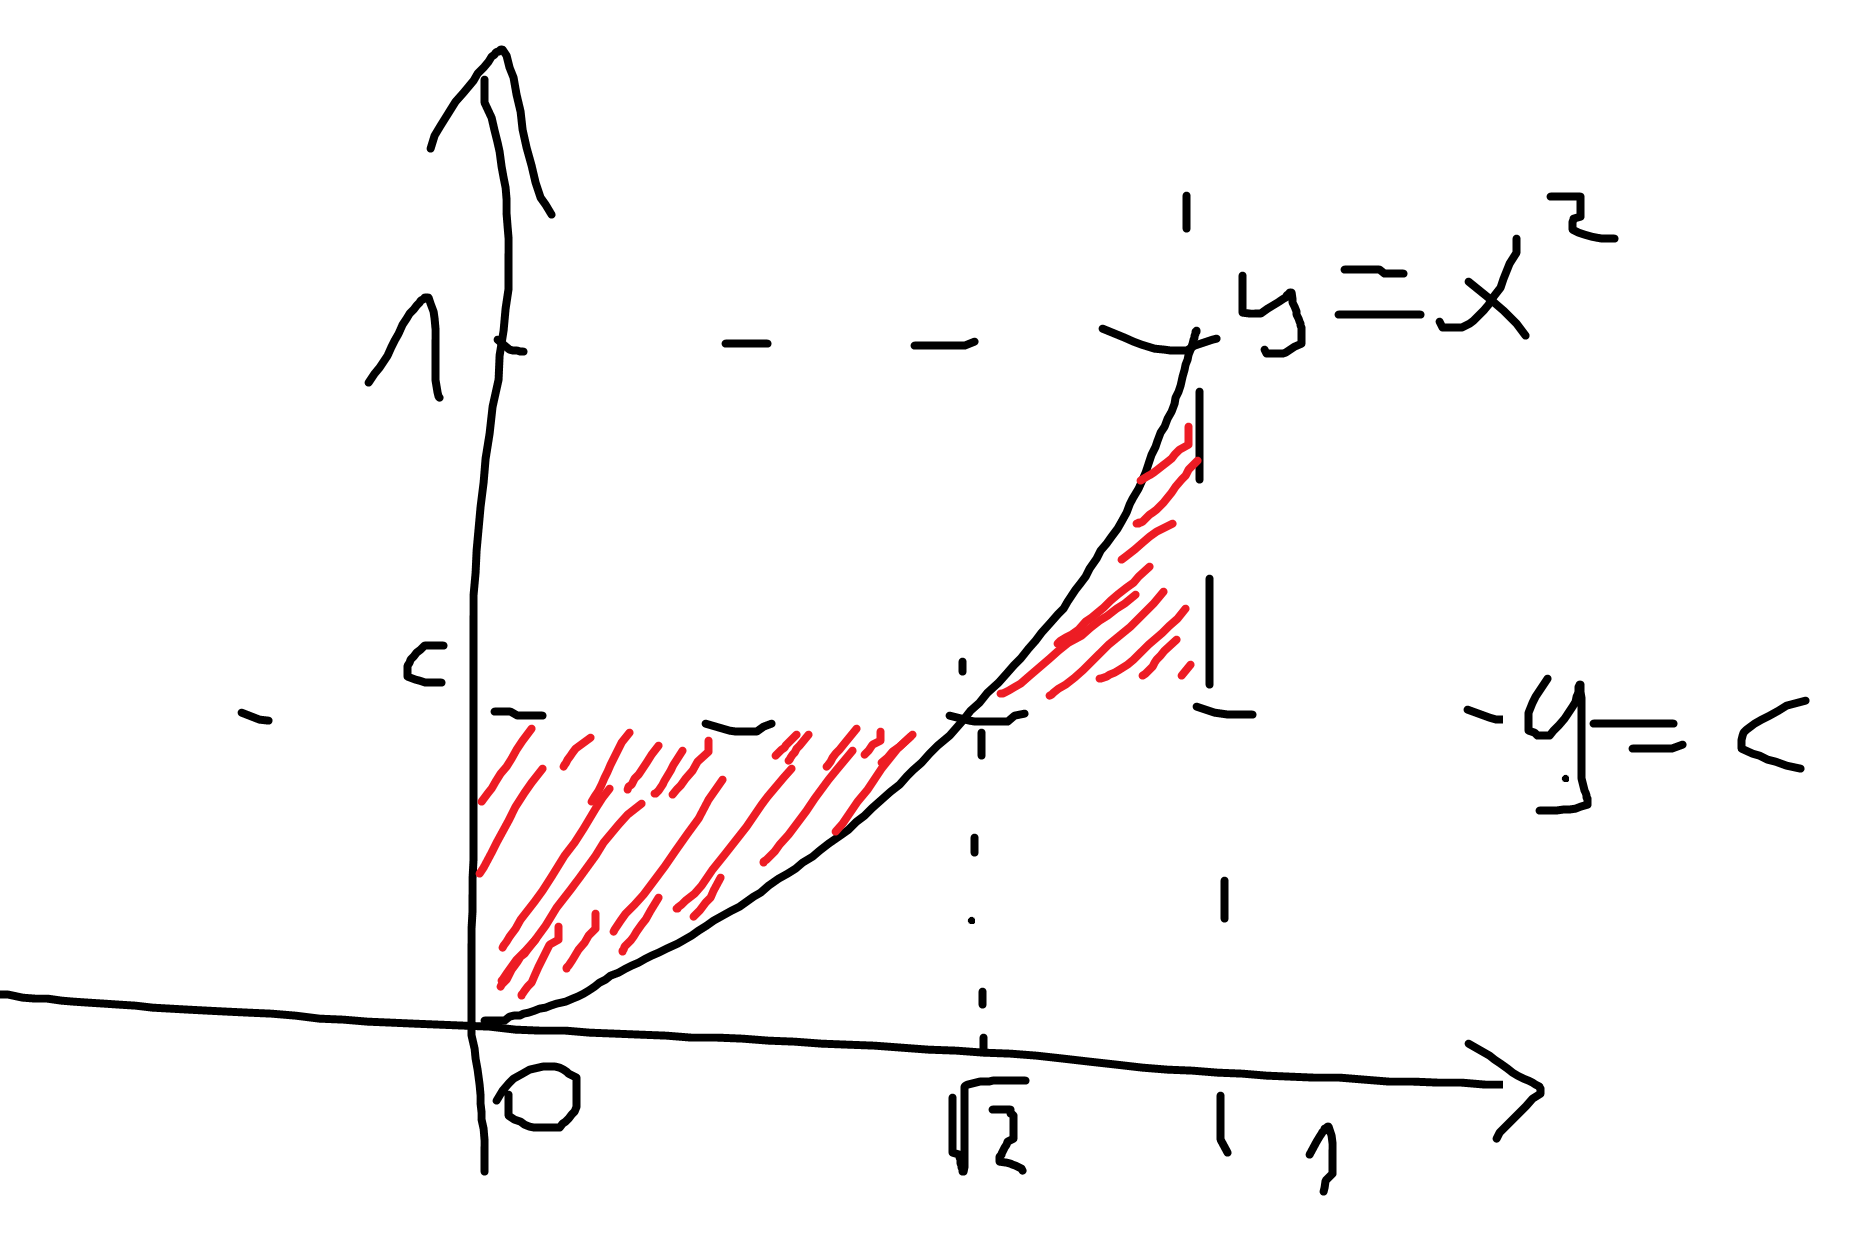
\includegraphics[height=3cm]{kepek/10.png}
			\caption{}
		\end{figure}
		
		Azaz, hogyan kell meghúzni az egyenest úgy, hogy a terület a legkisebb legyen? Világos, hogy elég $c\in[0,1]$ intervallumot vizsgálnunk, ui. ellenkező esetben 1-1 téglalap területével nő a terület.
		\smallskip
		
		Metszéspontok:
		\[ x^2=x\quad \Leftrightarrow\quad x=\pm\sqrt{c}\quad \Rightarrow\quad x=\sqrt{c}\in[0,1] \]
		Határozzuk meg a területet:
		\[ T(c)=\int_0^{\sqrt{c}}(c-x^2)\,dx+\int_{\sqrt{c}}^{1}(x^2-c)\,dx=\left[cx-\frac{x^3}{3}\right]_0^{\sqrt{c}}+\left[\frac{x^3}{3}-cx\right]^1_{\sqrt{c}}=c\sqrt{c}-\frac{c\sqrt{c}}{3}+\frac{1}{3}-c-\frac{c\sqrt{c}}{3}+c\sqrt{c}=\]
		\[=\frac{4}{3}c\sqrt{c}-c+\frac{1}{3}\quad c\in[0,1] \]
		Kompakt halmazon folytonos függvényt vizsgálunk, és kell hogy legyen maximum vagy minimum. Ez lehet 0 vagy 1, vagy intervallumon belül. Ha $c\in(0,1)$ akkor:
		\[T'(c)=\frac{4}{3}\cdot\frac{3}{2}\cdot\sqrt{c}-1=2\cdot\sqrt{c}-1=0\quad \Leftrightarrow\quad c=\frac{1}{4}\in(0,1)\checkmark \]
		\begin{center}		
			\begin{tabular}{l|c|c|c}
				$T'(x)$&$-$&0&$+$\\
				\hline
				$T(x)$&$\frac{1}{3}\searrow$&$\frac{1}{4}$&$\nearrow\frac{2}{3}$
			\end{tabular}
		\end{center}
		\[ T(0)=\frac{1}{3};\quad T(1)=\frac{2}{3};\quad T\left(\frac{1}{4}\right)=\frac{1}{4} \]
		Összefoglalva, a terület minimális a $c=\frac{1}{4}$ választással.
	\end{example}
	\begin{note}
		Mi ez a feladat? $f(x):=x^2, \quad x\in[0,1];\quad g(x):=c;\quad \rho_1(f,g):=\int_0^1|f-g|$
		\[ \Rightarrow\quad (C[0,1];\rho_1) \quad \text{m. tér};\quad \min\left\{\rho_1(f,g)\ | \ y=c\in\R\right\} \]
	\end{note}
	\subsubsection{Ívhossz számolás}
	\begin{note}
		$f\in C^1[a,b]$
		\begin{figure}[H]
			\centering
			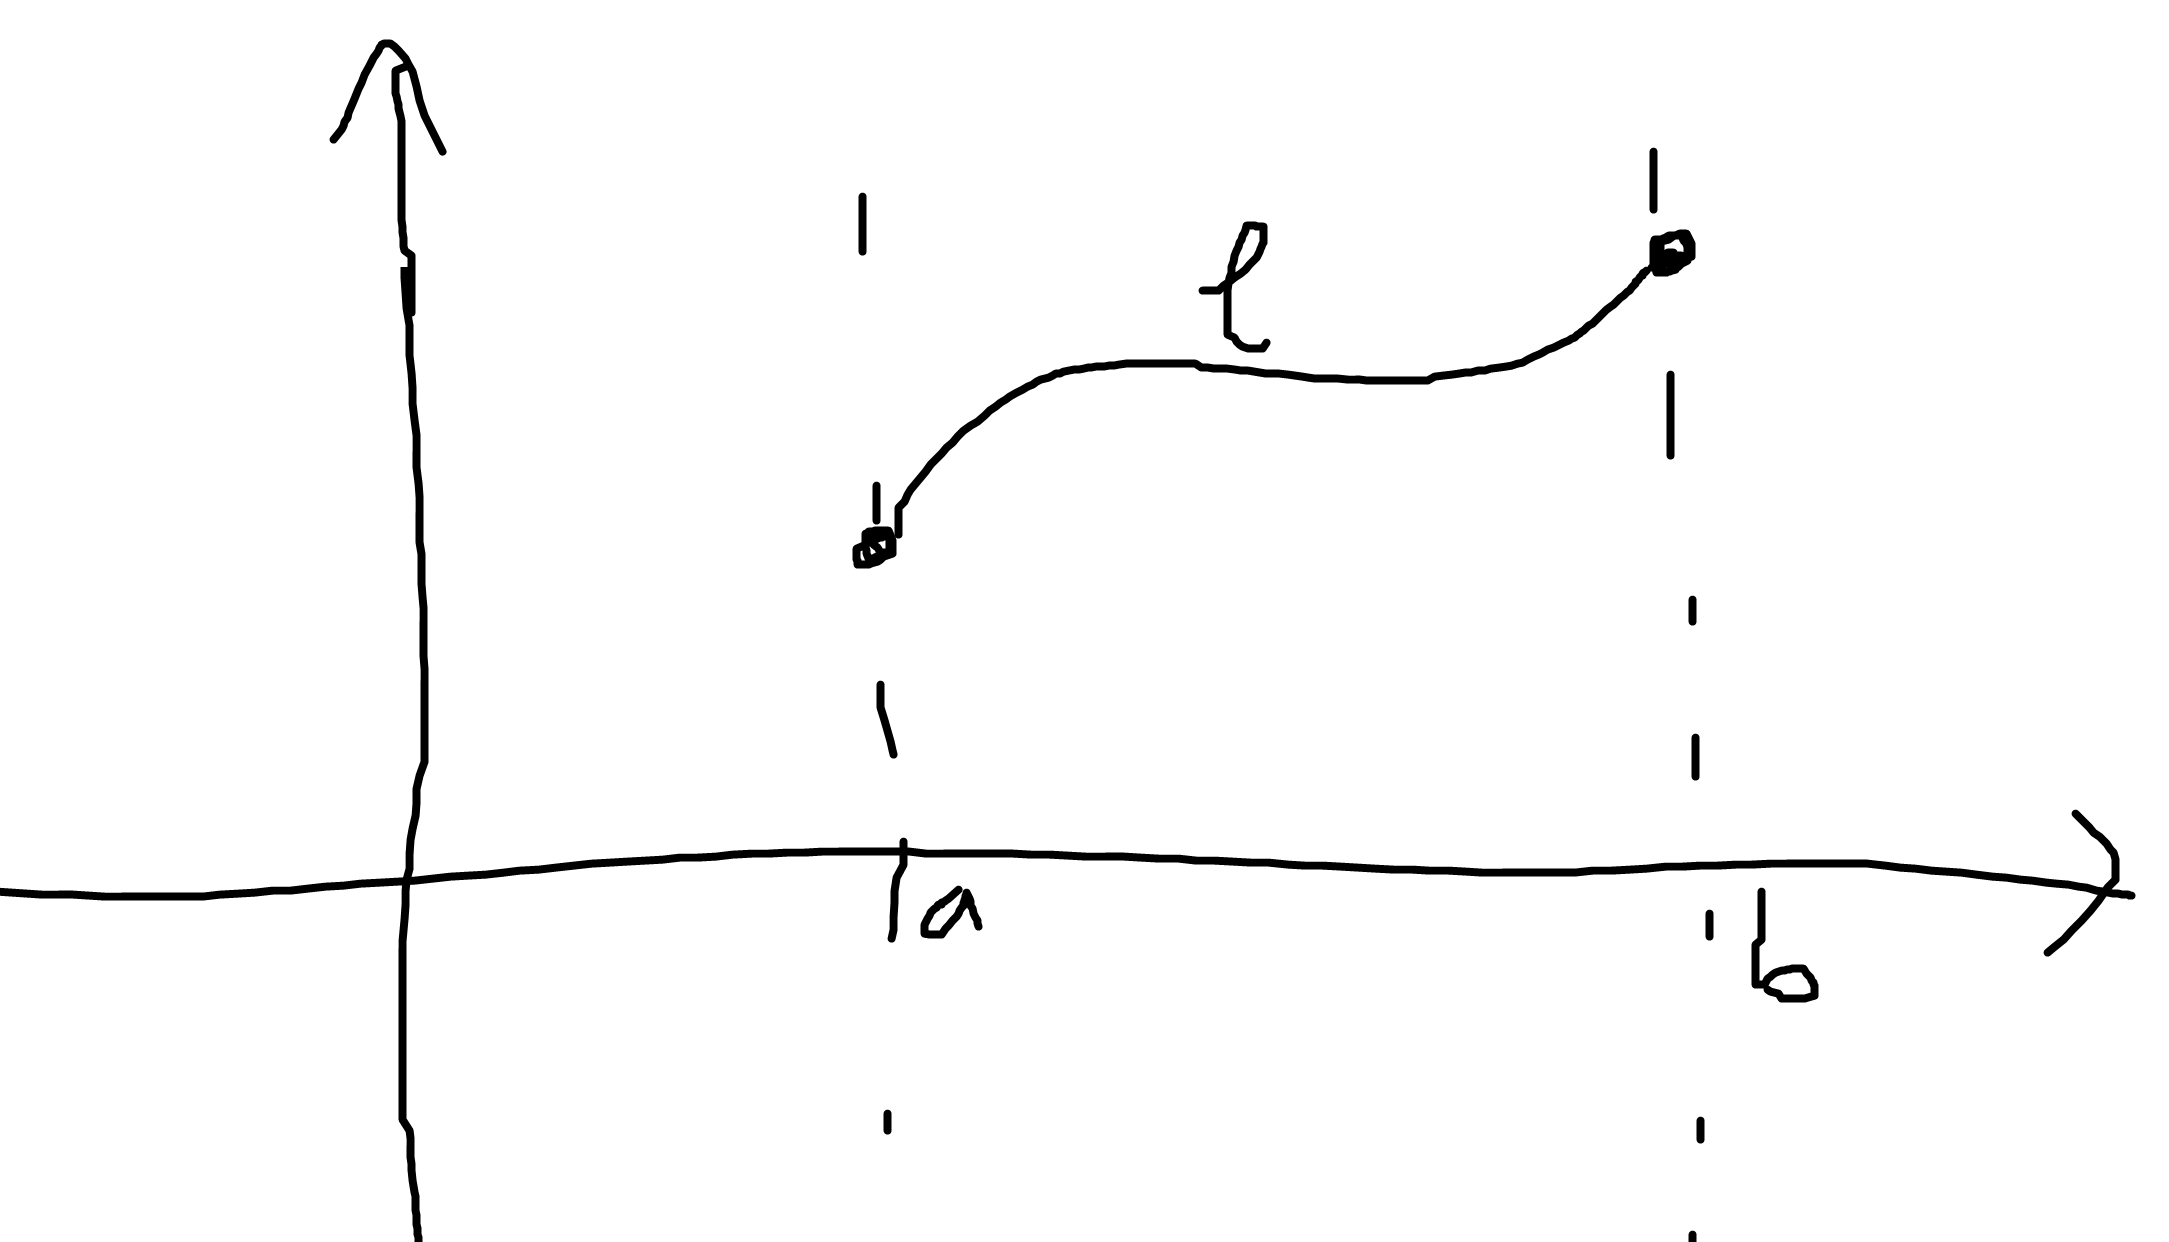
\includegraphics[height=3cm]{kepek/11.png}
			\caption{}
		\end{figure}
		\vspace{-6mm}
		\[ l=\int_a^b\sqrt{1+(f'(x))^2}\,dx \]
	\end{note}
	\begin{example}
		\[ f(x):=\frac{2(x-1)^{\frac{3}{2}}}{3};\quad x\in[2,5] \]
		Megoldás:
		\[ f'(x)=\frac{2}{3}\cdot\frac{3}{2}\cdot(x-1)^\frac{1}{2}=\sqrt{x-1} \]
		\[ \Rightarrow\quad l=\int_2^5\sqrt{1+x-1}\,dx=\int_2^5\sqrt{x}\,dx=\left[\frac{x^\frac{3}{2}}{\frac{3}{2}}\right]_2^5=\frac{2}{3}\left(5\sqrt{5}-2\sqrt{2}\right) \]
	\end{example}
	\begin{exercise}
		\[ f(x):=\sqrt{x};\quad x\in[1,2] \]
		Mekkora ívének hossza 1 és 2 között?
		\begin{figure}[H]
			\centering
			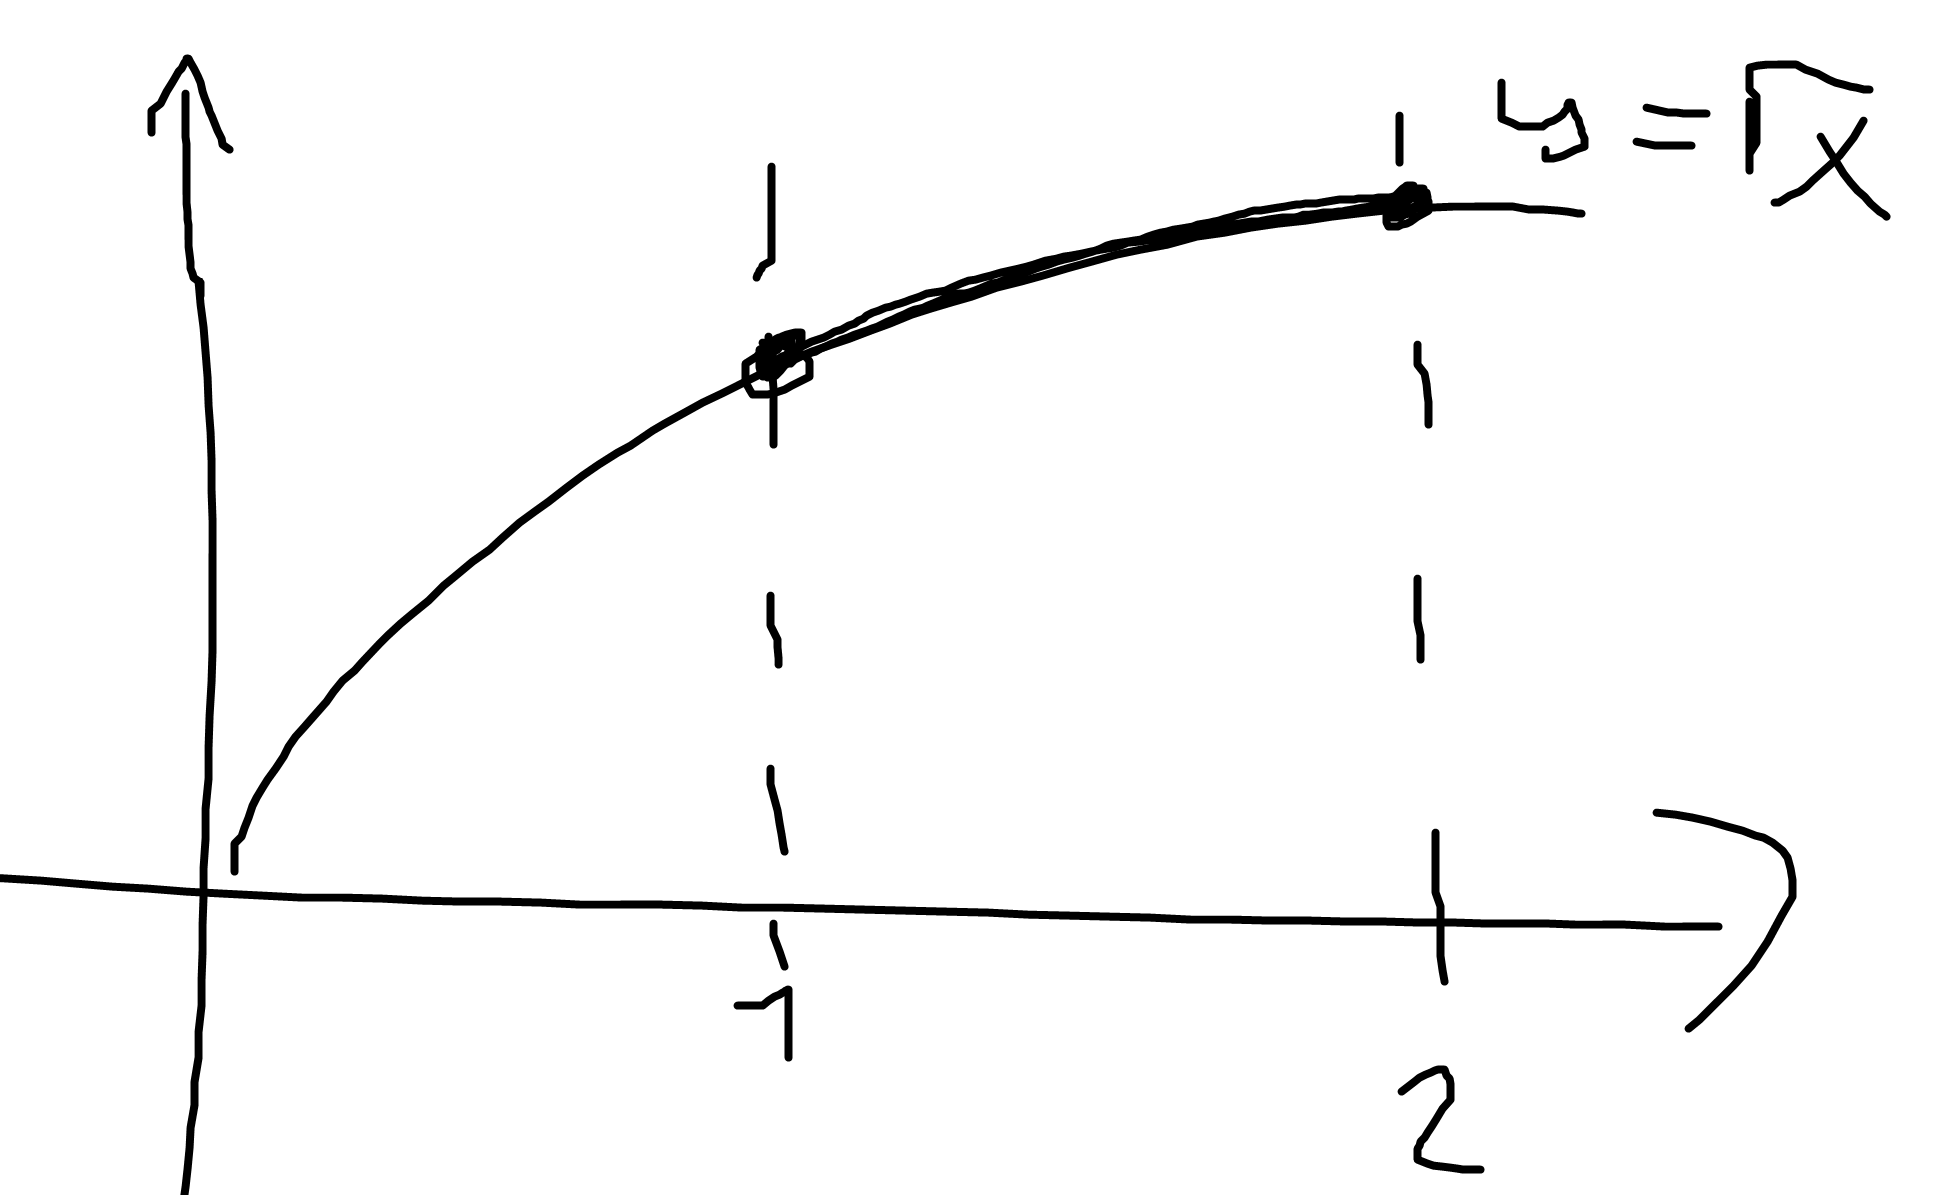
\includegraphics[height=3cm]{kepek/12.png}
			\caption{}
		\end{figure}
		Megoldás:
		\[ \Rightarrow\quad l=\int_1^2\sqrt{1+\left[(\sqrt{x}')\right]^2}\,dx=\int_1^2\sqrt{1+\left(\frac{1}{2\sqrt{x}}\right)^2}\,dx=\int_1^2\sqrt{1+\frac{1}{4x}}\,dx=\frac{1}{2}\cdot\int_1^2\sqrt{\frac{4x+1}{x}}\,dx= \]
		Vezessünk be egy új változót:
		\[ t:=\sqrt{\frac{4x+1}{x}},\quad x=\frac{1}{t^2-4},\quad dx=-\frac{2t}{(t^2-4)^2}\,dt\]
		Megállapítható, hogy 
		\[ x=1\quad \Rightarrow\quad t=\sqrt{5} \]
		\[ x=2\quad \Rightarrow\quad t=\frac{3}{\sqrt{2}} \]
		Visszatérve:
		\[ =-\frac{1}{2}\cdot\int_{\sqrt{5}}^{\frac{3}{\sqrt{2}}}t\left(\frac{2t}{(t^2-4)^2}\right)\,dt\quad \overset{\int_a^bf=-\int_b^af}{=}\quad \int_{\frac{3}{\sqrt{2}}}^{\sqrt{5}}\frac{t^2}{(t-2)^2(t+2)^2}\,dt=\]
		\[=\int_{\frac{3}{\sqrt{2}}}^{\sqrt{5}}\left(\frac{A}{t-2}+\frac{B}{(t-2)^2}+\frac{C}{t+2}+\frac{D}{(t+2)^2}\right)\,dt=\]
		\textit{A feladat befejezése:} Határozzuk meg $A,B,C,D\in\R$-t.
		\begin{align*}
			t^2\quad &=\quad A(t-2)(t+2)^2+B(t+2)^2+C(t+2)(t-2)^2+D(t-2)^2=\\
					 &=\quad A(t^2-4)(t+2)+B(t+2)^2+C(t^2-4)(t-2)+D(t-2)^2=\\
					 &=\quad A(t^3+2t^2-4t-8)+B(t^2+4t+4)+C(t^3-2t^2-4t+8)+D(t^2-4t+4)=\\
					 &=\quad (A+C)t^3+(2A+B-2C+D)t^2+(-4A+4B-4C-4D)t+(-8A+4B+8C+4D)
		\end{align*}
		\textit{Értékadással} könnyen megadható pár konstans.
		\begin{align*}
		t=-2\quad \Rightarrow&\quad 4=16D\quad \Leftrightarrow\quad D=\frac{1}{4}\\
		t=2\quad \Rightarrow &\quad 4=16B\quad \Leftrightarrow\quad B=\frac{1}{4}
		\end{align*}
		Így könnyebben számolható a többi konstans \textit{egyenlő együtthatók} módszerével.
		\begin{align*}
			t^3 \quad \text{együtthatója:}\quad 0&=A+C\\
			t^2 \quad \text{együtthatója:}\quad 
												1&=2A+\frac{1}{4}-2C+\frac{1}{4}\\
											   \frac{1}{4}&=A-C\\
			t^1 \quad \text{együtthatója:}\quad 0&=-4A+1-4C-1\\
												0&=-A-C\\
			t^0 \quad \text{együtthatója:}\quad 0&=-8A+1+8C+1\\
												1&=-4A+4C
		\end{align*}
		Ez alapján megállapítható hogy $C=-\frac{1}{8}$ és $A=\frac{1}{8}$. Visszatérve:
		\[=-\frac{1}{8}\cdot\int_{\frac{3}{\sqrt{2}}}^{\sqrt{5}}\frac{1}{t-2}\,dt+\frac{1}{4}\cdot\int_{\frac{3}{\sqrt{2}}}^{\sqrt{5}}\frac{1}{(t-2)^2}\,dt+\frac{1}{8}\cdot\int_{\frac{3}{\sqrt{2}}}^{\sqrt{5}}\frac{1}{t+2}\,dt+\frac{1}{4}\cdot\int_{\frac{3}{\sqrt{2}}}^{\sqrt{5}}\frac{1	}{(t+2)^2}\,dt=\]
		\[= \frac{1}{8}\left(-\Big[\ln(t-2)\Big]^{\sqrt{5}}_{\frac{3}{\sqrt{2}}}+2\left[-\frac{1}{1-2}\right]^{\sqrt{5}}_{\frac{3}{\sqrt{2}}}+\Big[\ln(t+2)\Big]^{\sqrt{5}}_{\frac{3}{\sqrt{2}}}+2\left[-\frac{1}{t+2}\right]^{\sqrt{5}}_{\frac{3}{\sqrt{2}}} \right)\]
		Megállapítható, hogy a területe létezik.~~~:)
	\end{exercise}
	\begin{note}
		Megállapítható, hogy $x^2$-te visszavezethető a $\sqrt{x}$ függvény.
		
		\begin{figure}[H]
			\centering
			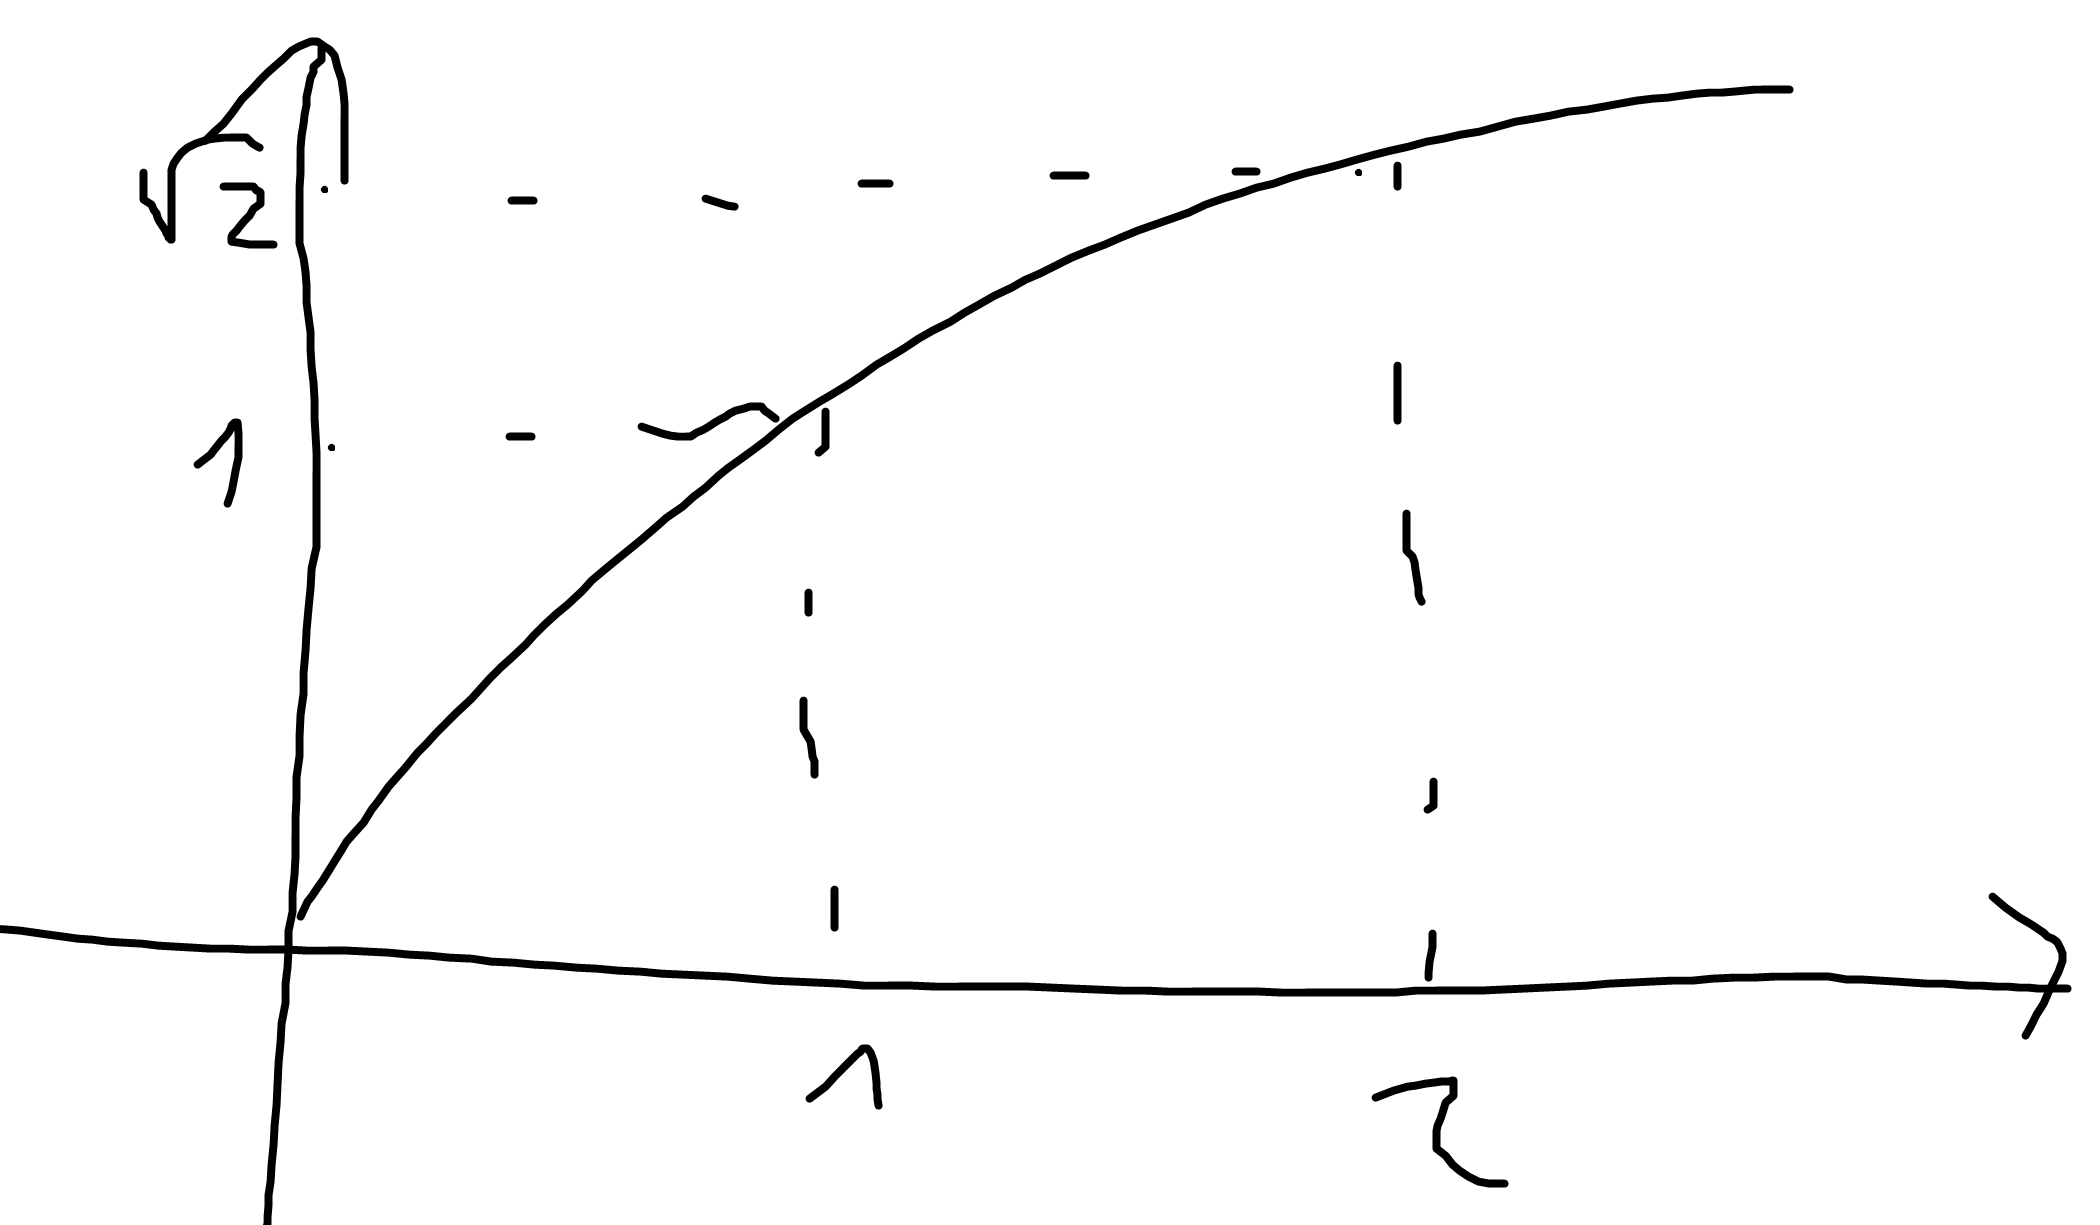
\includegraphics[height=3cm]{kepek/13.png}\quad \quad \quad 
			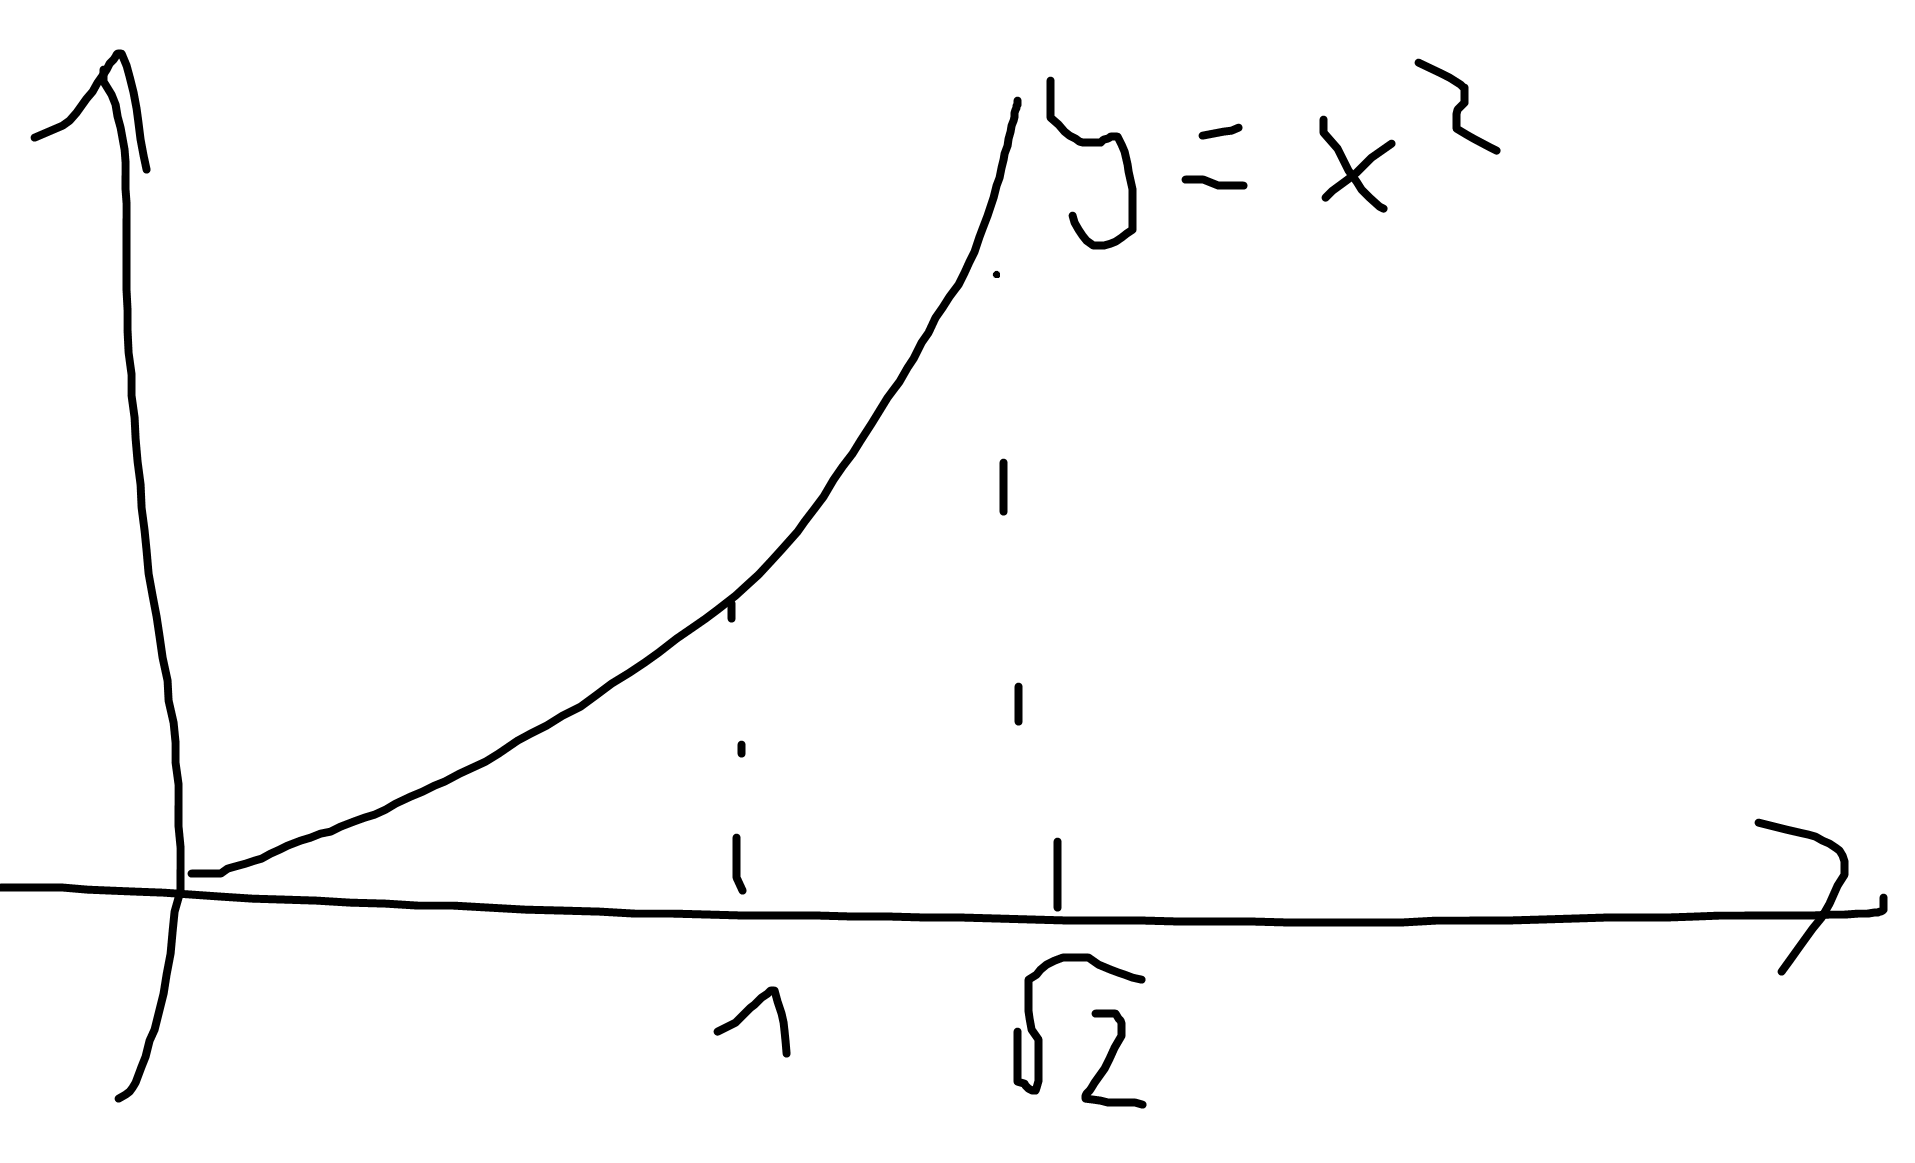
\includegraphics[height=3cm]{kepek/14.png}
			\caption{}
		\end{figure}
		\[ \Rightarrow\quad l=\int_1^{\sqrt{2}}\sqrt{1+4x^2}\,dx= \]
		Befejezése házi, javallott a $2x=\sh t$ helyettesítés.
	\end{note}
	\subsubsection{Forgástestek térfogata és felszíne}
	\begin{revision}
		\begin{figure}[H]
			\centering
			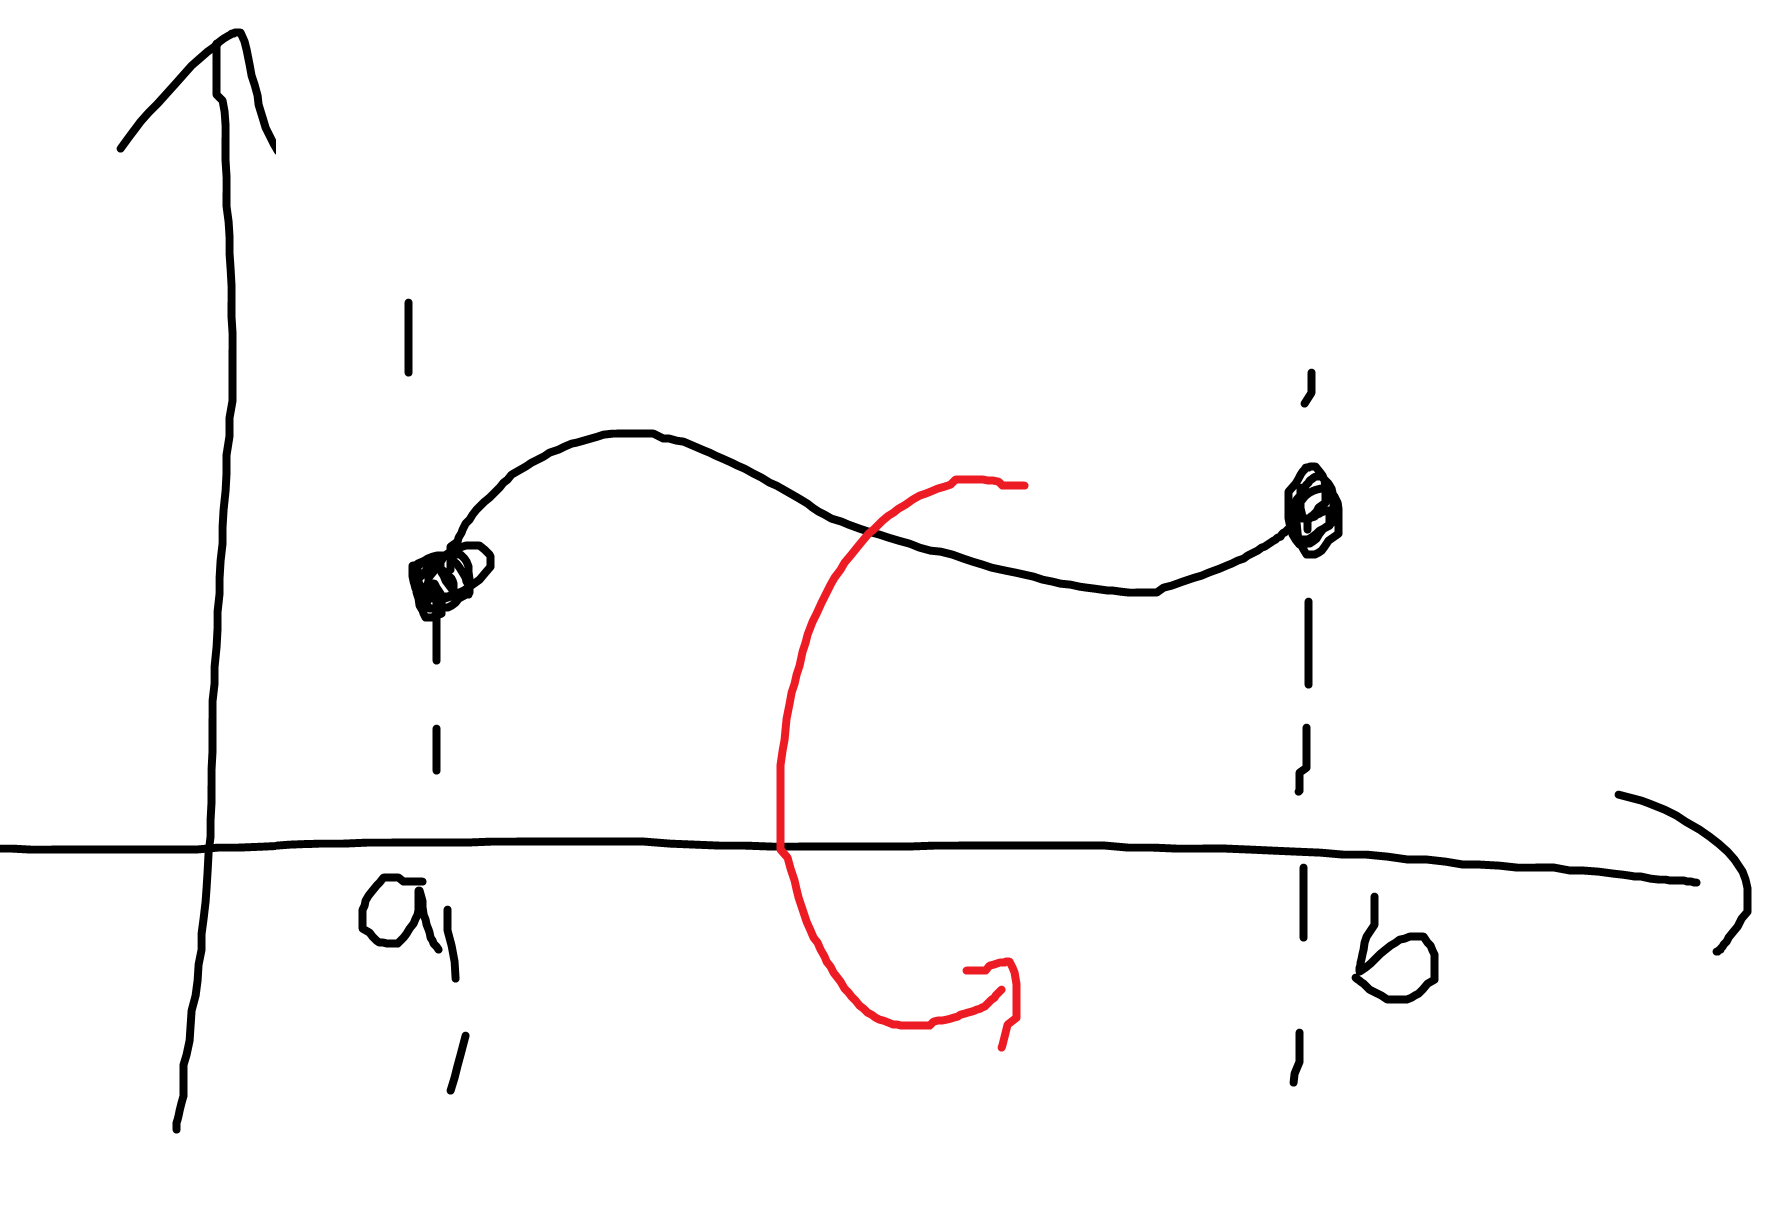
\includegraphics[height=3cm]{kepek/15pre.png}$\quad \quad \quad $
			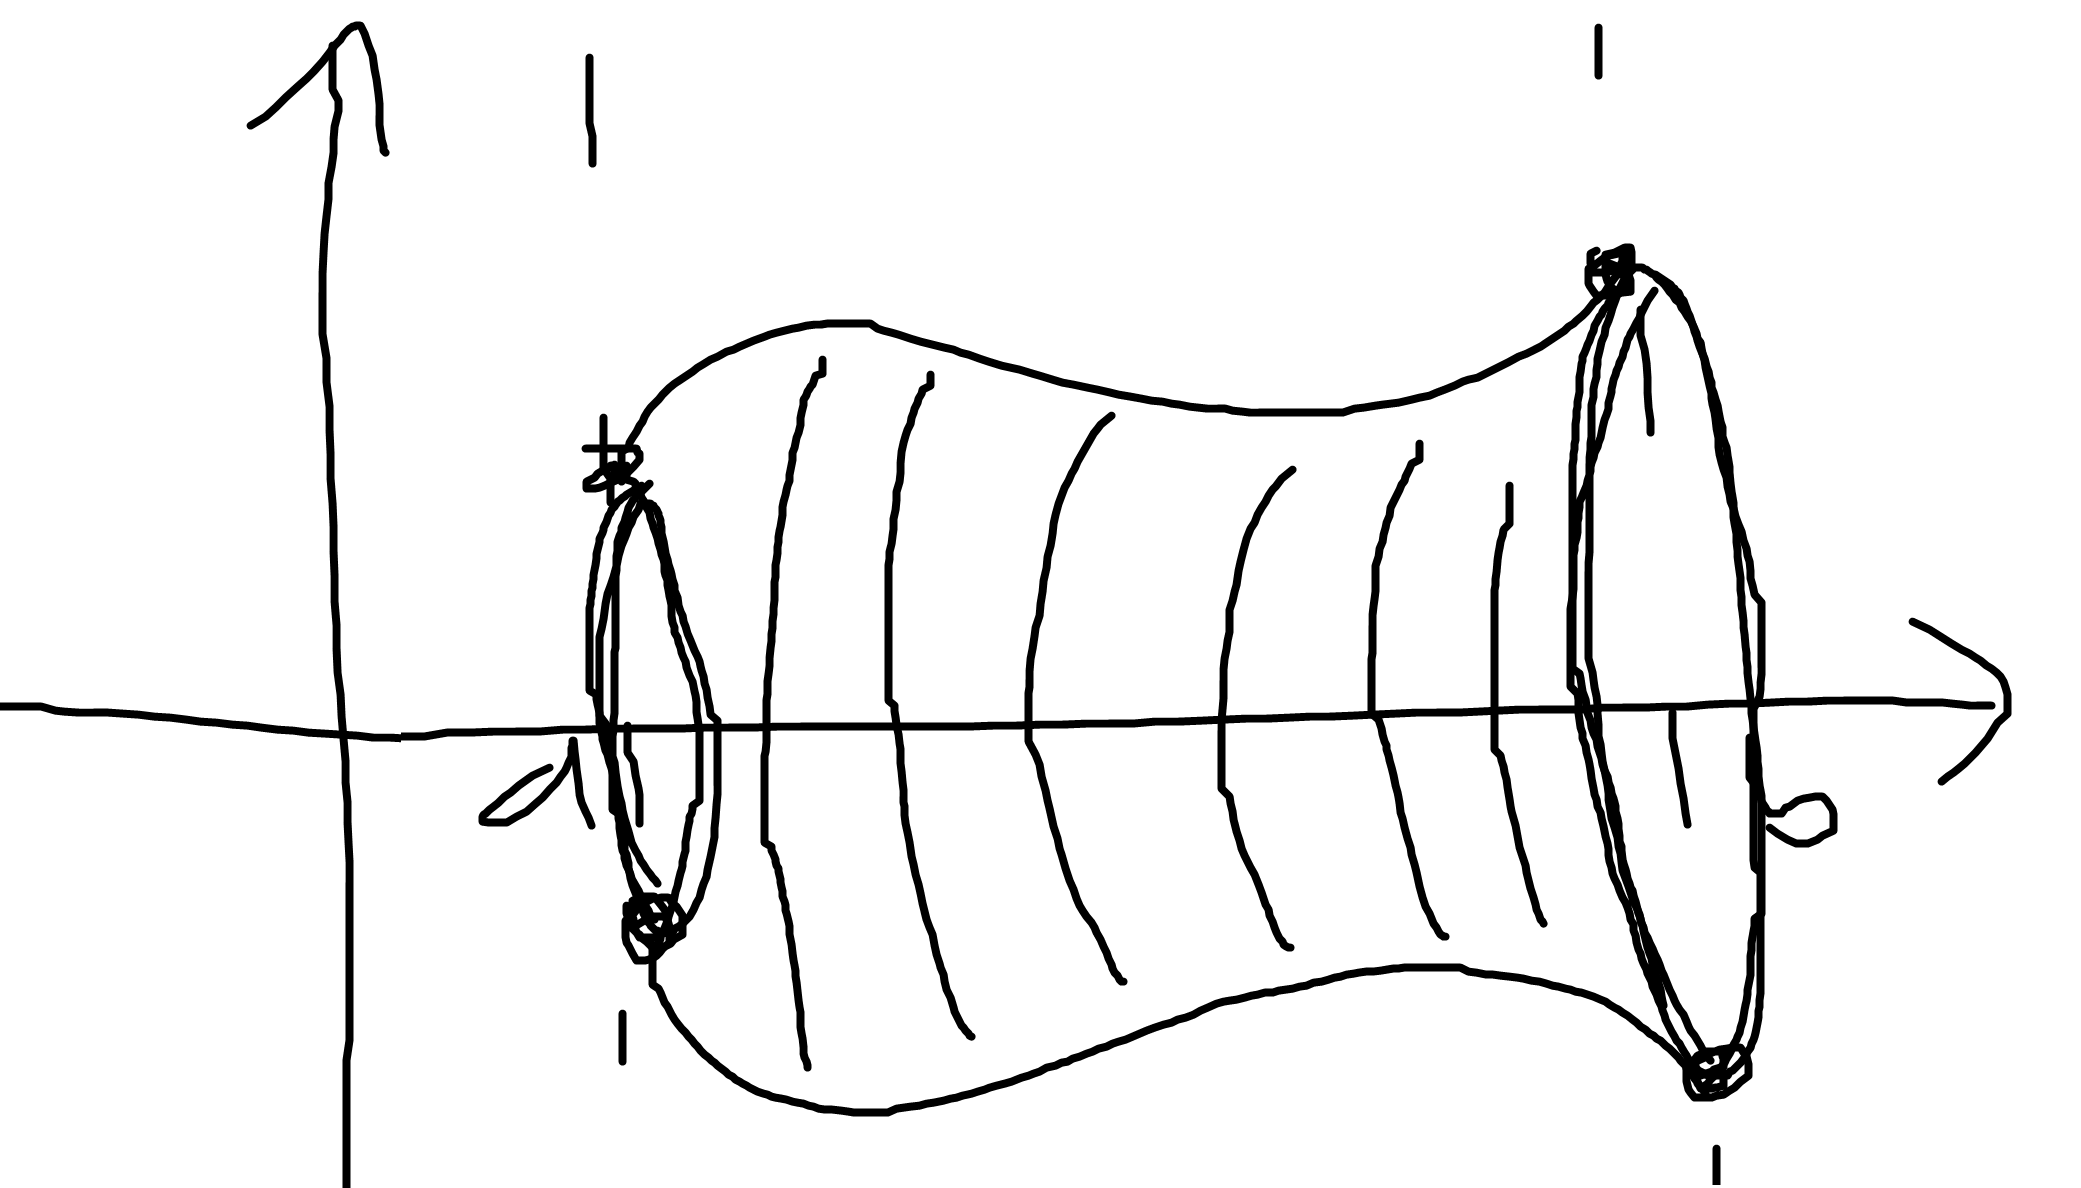
\includegraphics[height=3cm]{kepek/15.png}
			\caption{}\label{rotation}
		\end{figure}
		Ha a \ref{rotation}. ábrán lévő példát megforgatjuk az $x$ tengely körül, egy testet kapunk, melynek térfogatát számolhatjuk határozott integrállal.
		\[ V=\pi\int_a^bf^2(x)\,dx\quad (f\in\R[a,b]) \]
		\[ \mathcal{F}=2\pi\int_a^bf(x)\cdot\sqrt{1+(f'(x))^2}\,dx\quad (f\in C^1[a,b]) \]
		Ahol $V$ a térfogat (\textit{volume}) és $\mathcal{F}$ a felület.
	\end{revision}
	\begin{example} Határozzuk meg $f$ függvény $x$ tengely körüli forgástestének térfogatát ($V$), felületét ($\mathcal{F}$), és $f$ függvény alatti területét ($T$).
		\[ f(x):=\sin x\quad x\in[0,\pi]\]
		\begin{figure}[H]
			\centering
			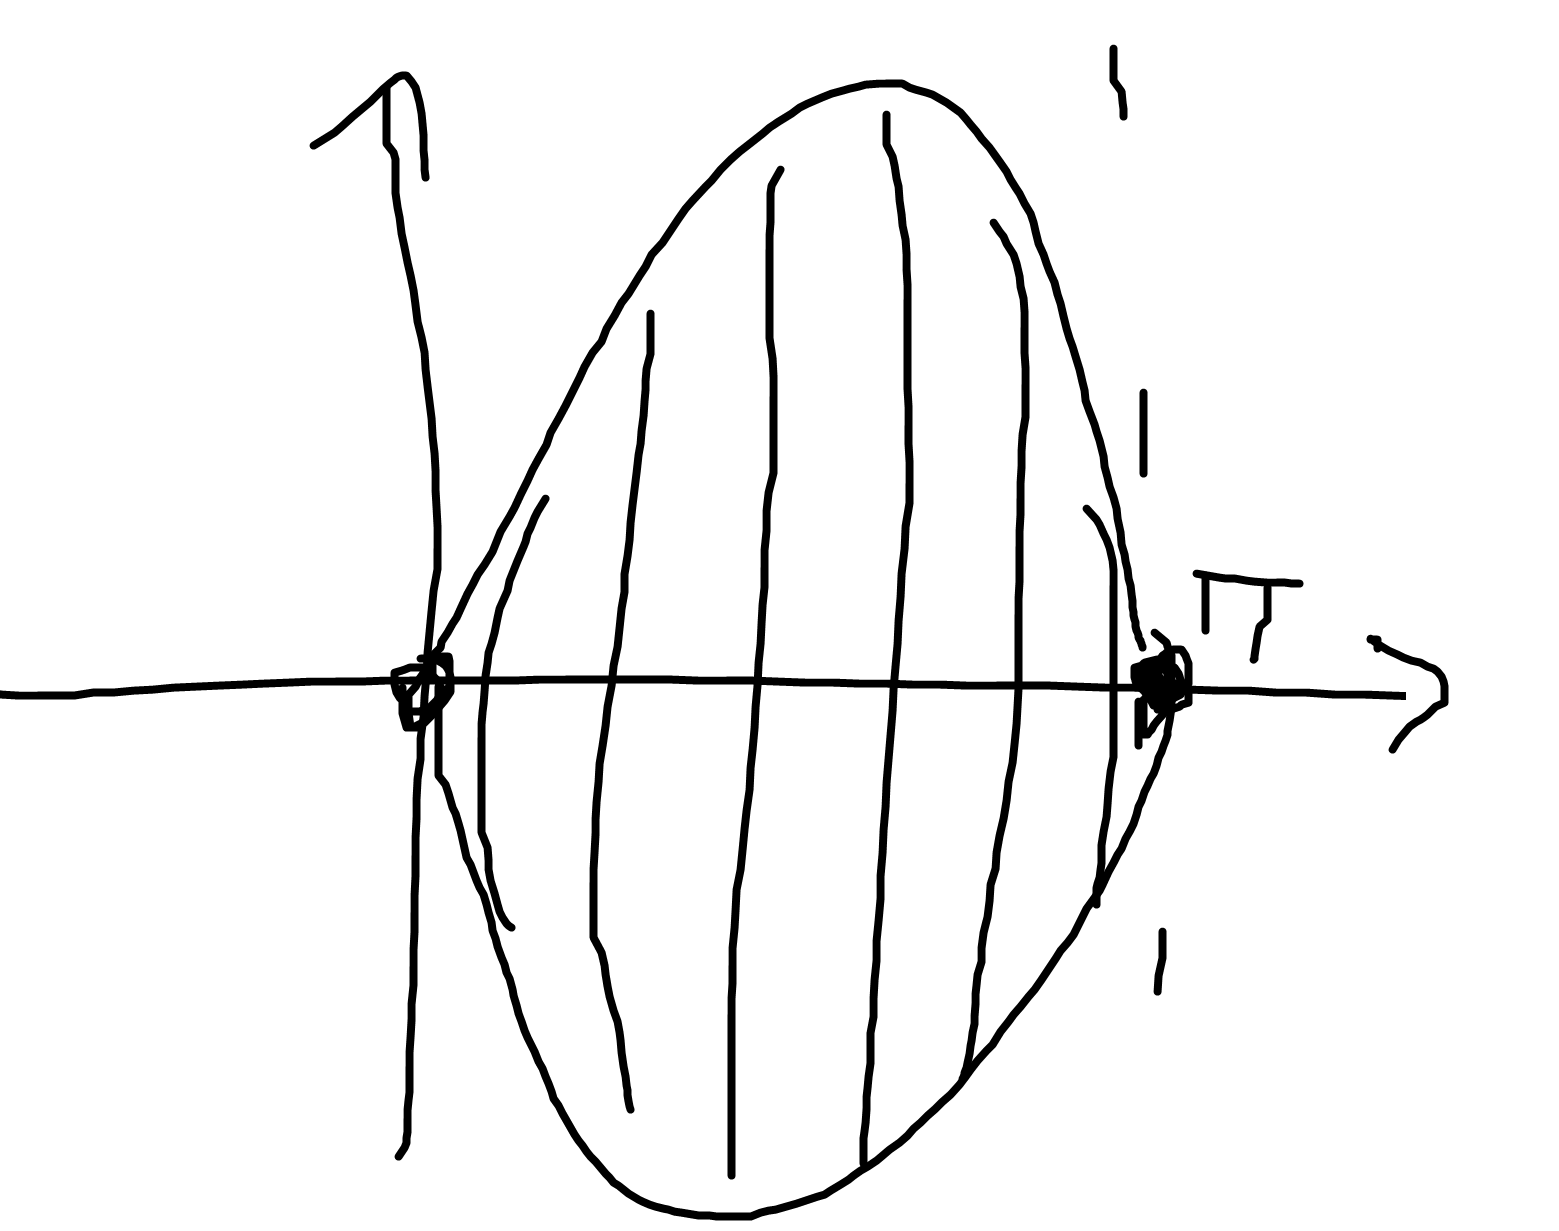
\includegraphics[height=3cm]{kepek/16.png}
			\caption{}
		\end{figure}
		\vspace{-6mm}
		\[ T=\int_0^\pi\sin x\,dx=\left[-\cos x\right]_0^\pi=1+\cos 0=2 \]
		\[ V=\pi\int_0^\pi\sin^2x\,dx=\frac{\pi}{2}\cdot\left[x-\frac{\sin2x}{2}\right]_0^\pi=\frac{\pi}{2}\cdot\left[\pi-\frac{\sin2\pi}{2}-0\right]=\frac{\pi^2}{2} \]
		Folytatván
		\[ \mathcal{F}=2\pi\cdot\int_0^\pi \sin x\cdot\sqrt{ 1+\cos^2x}\,dx= \]
		Vezessünk be egy új változót.
		\[ \sh t:=\cos x,\quad -\sin x\,dx=\ch t\,dt \]
		Visszatérve:
		\[ 2\pi\cdot\int \sin x\cdot\sqrt{ 1+\cos^2x}\,dx=2\pi\cdot\int\sqrt{1+\sh^2t}\cdot(-\ch t)\,dt \]
		\[ x=0\quad \Rightarrow\quad 1=\sh t\quad \Rightarrow\quad t=\arsh 1=\ln(\sqrt{2}+1) \]
		\[ x=\pi\quad \Rightarrow\quad -1=\sh t\quad \Rightarrow\quad t=\arsh (-1)=\ln(\sqrt{2}-1) \]
		\[ \arsh x=\ln(x+\sqrt{1+x^2}) \]
		Befejetése hf.
	\end{example}
	\begin{exercise}
		\[ f(x)=2\cdot\sqrt{1-x^2}\quad x\in[-1,1] \]
		Forgástest $V, \mathcal{F}=?$
		
		\[ y^2=2\sqrt{1-x^2}\quad \Rightarrow\quad \frac{y^2}{4}+x^2=1 \]
		\[ \frac{x^2}{a^2}+\frac{y^2}{b^2}=1 \]
	\end{exercise}
	\subsection{Összefoglaló}
	\subsubsection{$\sin, \ \cos$ azonosságok ($\forall x\in\R$)}
	\begin{align*}
		\sin^2x+\cos^2x&=1\\
		\cos^2x-\sin^2x&=\cos2x\\
		2\cos x\sin x&=\sin2x\\
		\frac{1+\cos2x}{2}&=\cos^2 x\\
		\frac{1-\cos2x}{2}&=\sin^2x
	\end{align*}
	A következő helyettesítéssel:
	\[  t:=\tg \left(\frac{x}{2}\right) \]
	Könnyen megállapítható hogy
	\[ \sin x=\frac{2t}{1+t^2}\quad \text{és}\quad  \cos x=\frac{1-t^2}{1+t^2} \]
	\subsubsection{$\sh, \ \ch$ azonosságok ($\forall x\in\R$)}
	\begin{align*}
		\frac{e^x+e^{-x}}{2}&=\ch x\\
		\frac{e^x-e^{-x}}{2}&=\sh x\\
		\ch^2x-\sh^2x&=1\\
		\frac{1+\ch2x}{2}&=\ch^2 x\\
		2\sh x\ch x&=\sh(2x)
	\end{align*}
	\subsubsection{$\ln$ azonosságok ($\forall a,b\in\R^+$)}
	\begin{align*}
		\ln(a^2)&=2\ln a\\
		\ln(a)-\ln(b)&=\ln\left(\frac{a}{b}\right)\\
		\ln(a)+\ln(b)&=\ln(a\cdot b)
	\end{align*}
	\subsubsection{Integrálazonosságok}
	Legyen $f\in\R\to\R$, $F$ legyen $f$ primitív függvénye. Legyen továbbá $f\in D$.
	\[ \int\frac{f'(x)}{f(x)}\,dx=\ln|f(x)|+c\quad (x,c\in\R) \]
	\[ \int f'(x)\cdot f^\alpha(x)\,dx=\frac{f^{\alpha+1}}{\alpha+1}+c\quad (x,c\in\R) \]
	Racionális törtfüggvény nevezőjében másodfokú irreducibilis polinom $n$-edik hatványához tartozó rekurzív formula:
	\[ I_n(x):=\int\frac{1}{(1+x^2)^n}\,dx=\frac{1}{2(n-1)}\cdot\frac{x}{(1+x^2)^{n-1}}+\frac{2n-3}{2(n-1)}\cdot I_{n-1}(x) \]
	Speciális esetben, ha $n=2$:
	\[ I_2(x):=\int\frac{1}{(1+x^2)^2}\,dx=\frac{1}{2}\cdot\frac{x}{1+x^2}+\frac{1}{2}\arc\tg x+c\quad (c\in\R) \]
	\subsubsection{Határozott integrál}
	A terület ($T$), térfogat ($x$ tengely körüli forgatáskor keletkező forgástest, $V$), felület ($\mathcal{F}$) és ívhossz ($l$) meghatározása $a,b\in\R$ intervallumon:
	\[ T=\int_a^bf(x)\,dx\quad (f\in\R[a,b]) \]
	\[ V=\pi\int_a^bf^2(x)\,dx\quad (f\in\R[a,b]) \]
	\[ \mathcal{F}=2\pi\int_a^bf(x)\cdot\sqrt{1+(f'(x))^2}\,dx\quad (f\in C^1[a,b]) \]
	\[ l=\int_a^b\sqrt{1+(f'(x))^2}\,dx \]
\end{document}
